\documentclass[a4paper, 11pt, openbib, oldfontcommands]{memoir}

\usepackage[ED=MITT-STICIA, Ets=UT3]{tlsflyleaf}

\usepackage{datetime}
\usepackage{ifpdf} % For pdf metadata
% The import command enables each chapter tex file to use relative paths when
% accessing supplementary files. For example, to include
% chapters/brewing/images/figure1.png from chapters/brewing/brewing.tex we can
% use \includegraphics{images/figure1} instead of
% \includegraphics{chapters/brewing/images/figure1}
\usepackage{import}

\usepackage[]{lipsum}
\usepackage{color} % Creates coloured text and background
\usepackage{footnote}	% For footnotes
\usepackage{microtype}% Makes pdf look better.
\usepackage{lettrine} % For initial letters
\usepackage[version=0.96]{pgf} % For chapter style
\usepackage{calc, soul} % For Chapter style

% Oscar's command (it works): Fills blank pages until next odd-numbered page.
% Used to emulate single-sided frontmatter. This will work for title, abstract
% and declaration. Though the contents sections will each start on an
% odd-numbered page they will spill over onto the even-numbered pages if
% extending beyond one page (hopefully, this is ok).
\newcommand{\clearemptydoublepage}{\newpage{\thispagestyle{empty}\cleardoublepage}}

% My caption style
\newcommand{\mycaption}[2][\@empty]{
	\captionnamefont{\scshape}
	\changecaptionwidth
	\captionwidth{0.9\linewidth}
	\captiondelim{.\:}
	\indentcaption{0.75cm}
	\captionstyle[\centering]{}
	\setlength{\belowcaptionskip}{10pt}
	\ifx \@empty#1 \caption{#2}\else \caption[#1]{#2}
}

% My subcaption style
\newcommand{\mysubcaption}[2][\@empty]{
	\subcaptionsize{\small}
	\hangsubcaption
	\subcaptionlabelfont{\rmfamily}
	\sidecapstyle{\raggedright}
	\setlength{\belowcaptionskip}{10pt}
	\ifx \@empty#1 \subcaption{#2}\else \subcaption[#1]{#2}
}

%An initial of the very first character of the content
\newcommand{\initial}[1]{%
	\lettrine[lines=3,lhang=0.33,nindent=0em]{
		\color{gray}
     		{\textsc{#1}}}{}}

\def\vdotfill#1{\vtop to0pt{\null \dimen0=#1\baselineskip\advance\dimen0 by-.4ex 
   \kern-1.6ex \cleaders\hbox{\lower.4ex\vbox to1ex{}.}\vskip\dimen0 \vss}}

\newcommand{\aggr}[1]{\underset{#1}{\operatorname{aggr}}\;}
\newcommand{\rui}{r_{ui}}
\newcommand{\ruj}{r_{uj}}
\newcommand{\rvi}{r_{vi}}
\newcommand{\predrui}{\hat{r}_{ui}}
\newcommand{\predruj}{\hat{r}_{uj}}
\newcommand{\Iu}{I_u}
\newcommand{\Ui}{U_i}
\newcommand{\Uij}{U_{ij}}
\newcommand{\Iuv}{I_{uv}}
\newcommand{\Rtrain}{R_{\text{train}}}
\newcommand{\Rtest}{R_{\text{test}}}
\newcommand{\ssim}{\text{sim}} % similarity... \sim already exists
\newcommand{\clonedist}{\text{Clone\_dist}} % clone dist
\newcommand{\clonesim}{\text{Clone\_sim}} % clone sim

\newcommand*\albl[1]{\overline{f}(#1)}
\newcommand*\nan[0]{1\text{-nan}} %pour 1nan
\newcommand*\nanemph[0]{1\emph{-nan}} %pour 1nan dans une def ou une prop
\newcommand*\knan[0]{k\text{-nan}} %pour knan
\newcommand*\knn[0]{k\text{-nn}} %pour knn
\newcommand*\NAN[0]{\mbox{NAN}} %pour NaN
\newcommand*\nn[0]{1\mbox{-nn}} %pour 1nn
\newcommand*\NN[0]{\text{NN}} %pour NN
\newcommand*\acc[0]{\mbox{Acc}} %pour Acc
\newcommand\given[1][]{\:#1\vert\:} %pour proba conditionnelle
% pour equal by def
\newcommand\eqdef{\mathrel{\overset{\makebox[0pt]{\mbox{\normalfont\tiny\sffamily
def}}}{=}}}
\newcommand\numberthis{\addtocounter{equation}{1}\tag{\theequation}} % sais pas
\newcommand*\aext[2]{\mathbf{E}_{#1}^{#2}} % Analogical extension
\newcommand*\esf[0]{\mathbf{E}_{S}^{f}} % Analogical extension
\newcommand*\esfs[0]{\mathbf{E}_{S}^{f*}} % Analogical extension star
\newcommand*\aroot[3]{\mathbf{R}_{#1}^{#2}(#3)} % Analogical root
\newcommand*\rsfx[0]{\mathbf{R}_{S}^{f}(\mathbf{x})} % Analogical extension
\newcommand*\sol[0]{\text{sol}} % solution
\newcommand*\solvable[0]{\text{solvable}} % solvable
\newcommand*\AD[0]{\text{AD}} % Analogical Dissimilarity
\newcommand{\norm}[2]{{\left\lVert#2\right\rVert}_{#1}} % Norm definition
\newcommand*\omegasf[0]{\omega_{S}^{f}} % omega
\newcommand*\surpmax[0]{\text{Surp}^{\text{max}}} % surp max
\newcommand*\surpavg[0]{\text{Surp}^{\text{avg}}} % surp avg
\newcommand*\supp[0]{\text{supp}} % support
\newcommand*\knns[0]{k\text{-NN}^*} % knn star (with baseline)
\newcommand*\FCP[0]{\text{FCP}} % FCP
\newcommand*\bin[0]{\text{bin}} % bin
\newcommand*\binemph[0]{\emph{bin}} % binemph

\DeclareMathOperator*{\argmin}{arg\,min}
\DeclareMathOperator*{\argmax}{arg\,max}
\DeclareMathOperator*{\plim}{\mathit{p}-lim}
\newcommand{\pluseq}{\mathrel{+}=} % +=
\DeclareMathOperator{\ess}{ess}

% For vertical and horizontal bars in matrices
\newcommand*{\vertbar}{\rule[-1ex]{0.5pt}{2.5ex}}
\newcommand*{\horzbar}{\rule[.5ex]{2.5ex}{0.5pt}}

\theoremstyle{plain}  % Will be in italic
\newtheorem{proposition}{Proposition}[chapter]
\newtheorem{property}{Property}[chapter]

\theoremstyle{definition}  % Will not be italic
\newtheorem{definition}{Definition}[chapter]
\newtheorem{example}{Example}[chapter]

% For signed quote env
\def\signed #1{{\leavevmode\unskip\nobreak\hfil\penalty50\hskip2em
\hbox{}\nobreak\hfil(#1)%
\parfillskip=0pt \finalhyphendemerits=0 \endgraf}}
\newsavebox\mybox \newenvironment{aquote}[1]
{\savebox\mybox{#1}\begin{quote}}
{\signed{\usebox\mybox}\end{quote}}

% EXAMPLE environment
\newcounter{testexample}
\def\exampletext{Example} % If English
\NewDocumentEnvironment{testexample}{ O{} }
{
\colorlet{colexam}{black} % Global example color
\newtcolorbox[use counter=testexample]{testexamplebox}{%
    % Example Frame Start
    empty,% Empty previously set parameters
    title={\exampletext: #1},% use \thetcbcounter to access the testexample counter text
    % Attaching a box requires an overlay
    attach boxed title to top left,
       % Ensures proper line breaking in longer titles
       minipage boxed title,
    % (boxed title style requires an overlay)
    boxed title style={empty,size=minimal,toprule=0pt,top=4pt,left=3mm,overlay={}},
    coltitle=colexam,fonttitle=\bfseries,
    before=\par\medskip\noindent,parbox=false,boxsep=0pt,left=3mm,right=0mm,top=2pt,breakable,pad at break=0mm,
       before upper=\csname @totalleftmargin\endcsname0pt, % Use instead of parbox=true. This ensures parskip is inherited by box.
    % Handles box when it exists on one page only
    overlay unbroken={\draw[colexam,line width=.5pt] ([xshift=-0pt]title.north west) -- ([xshift=-0pt]frame.south west); },
    % Handles multipage box: first page
    overlay first={\draw[colexam,line width=.5pt] ([xshift=-0pt]title.north west) -- ([xshift=-0pt]frame.south west); },
    % Handles multipage box: middle page
    overlay middle={\draw[colexam,line width=.5pt] ([xshift=-0pt]frame.north west) -- ([xshift=-0pt]frame.south west); },
    % Handles multipage box: last page
    overlay last={\draw[colexam,line width=.5pt] ([xshift=-0pt]frame.north west) -- ([xshift=-0pt]frame.south west); },%
    }
\begin{testexamplebox}}
{\end{testexamplebox}\endlist}


\newcommand{\repeatcaption}[2]{%
  \renewcommand{\thefigure}{\ref{#1}}%
  \captionsetup{list=no}%
  \caption{#2 (repeated from page \pageref{#1})}%
}


\usepackage[ED=MITT-STICIA, Ets=UT3]{tlsflyleaf}

\usepackage{datetime}
\usepackage{ifpdf} % For pdf metadata
% The import command enables each chapter tex file to use relative paths when
% accessing supplementary files. For example, to include
% chapters/brewing/images/figure1.png from chapters/brewing/brewing.tex we can
% use \includegraphics{images/figure1} instead of
% \includegraphics{chapters/brewing/images/figure1}
\usepackage{import}

\usepackage[]{lipsum}
\usepackage{color} % Creates coloured text and background
\usepackage{footnote}	% For footnotes
\usepackage{microtype}% Makes pdf look better.
\usepackage{lettrine} % For initial letters
\usepackage[version=0.96]{pgf} % For chapter style
\usepackage{calc, soul} % For Chapter style

% Oscar's command (it works): Fills blank pages until next odd-numbered page.
% Used to emulate single-sided frontmatter. This will work for title, abstract
% and declaration. Though the contents sections will each start on an
% odd-numbered page they will spill over onto the even-numbered pages if
% extending beyond one page (hopefully, this is ok).
\newcommand{\clearemptydoublepage}{\newpage{\thispagestyle{empty}\cleardoublepage}}

% My caption style
\newcommand{\mycaption}[2][\@empty]{
	\captionnamefont{\scshape}
	\changecaptionwidth
	\captionwidth{0.9\linewidth}
	\captiondelim{.\:}
	\indentcaption{0.75cm}
	\captionstyle[\centering]{}
	\setlength{\belowcaptionskip}{10pt}
	\ifx \@empty#1 \caption{#2}\else \caption[#1]{#2}
}

% My subcaption style
\newcommand{\mysubcaption}[2][\@empty]{
	\subcaptionsize{\small}
	\hangsubcaption
	\subcaptionlabelfont{\rmfamily}
	\sidecapstyle{\raggedright}
	\setlength{\belowcaptionskip}{10pt}
	\ifx \@empty#1 \subcaption{#2}\else \subcaption[#1]{#2}
}

%An initial of the very first character of the content
\newcommand{\initial}[1]{%
	\lettrine[lines=3,lhang=0.33,nindent=0em]{
		\color{gray}
     		{\textsc{#1}}}{}}

\def\vdotfill#1{\vtop to0pt{\null \dimen0=#1\baselineskip\advance\dimen0 by-.4ex 
   \kern-1.6ex \cleaders\hbox{\lower.4ex\vbox to1ex{}.}\vskip\dimen0 \vss}}

\newcommand{\aggr}[1]{\underset{#1}{\operatorname{aggr}}\;}
\newcommand{\rui}{r_{ui}}
\newcommand{\ruj}{r_{uj}}
\newcommand{\rvi}{r_{vi}}
\newcommand{\predrui}{\hat{r}_{ui}}
\newcommand{\predruj}{\hat{r}_{uj}}
\newcommand{\Iu}{I_u}
\newcommand{\Ui}{U_i}
\newcommand{\Uij}{U_{ij}}
\newcommand{\Iuv}{I_{uv}}
\newcommand{\Rtrain}{R_{\text{train}}}
\newcommand{\Rtest}{R_{\text{test}}}
\newcommand{\ssim}{\text{sim}} % similarity... \sim already exists
\newcommand{\clonedist}{\text{Clone\_dist}} % clone dist
\newcommand{\clonesim}{\text{Clone\_sim}} % clone sim

\newcommand*\albl[1]{\overline{f}(#1)}
\newcommand*\nan[0]{1\text{-nan}} %pour 1nan
\newcommand*\nanemph[0]{1\emph{-nan}} %pour 1nan dans une def ou une prop
\newcommand*\knan[0]{k\text{-nan}} %pour knan
\newcommand*\knn[0]{k\text{-nn}} %pour knn
\newcommand*\NAN[0]{\mbox{NAN}} %pour NaN
\newcommand*\nn[0]{1\mbox{-nn}} %pour 1nn
\newcommand*\NN[0]{\text{NN}} %pour NN
\newcommand*\acc[0]{\mbox{Acc}} %pour Acc
\newcommand\given[1][]{\:#1\vert\:} %pour proba conditionnelle
% pour equal by def
\newcommand\eqdef{\mathrel{\overset{\makebox[0pt]{\mbox{\normalfont\tiny\sffamily
def}}}{=}}}
\newcommand\numberthis{\addtocounter{equation}{1}\tag{\theequation}} % sais pas
\newcommand*\aext[2]{\mathbf{E}_{#1}^{#2}} % Analogical extension
\newcommand*\esf[0]{\mathbf{E}_{S}^{f}} % Analogical extension
\newcommand*\esfs[0]{\mathbf{E}_{S}^{f*}} % Analogical extension star
\newcommand*\aroot[3]{\mathbf{R}_{#1}^{#2}(#3)} % Analogical root
\newcommand*\rsfx[0]{\mathbf{R}_{S}^{f}(\mathbf{x})} % Analogical extension
\newcommand*\sol[0]{\text{sol}} % solution
\newcommand*\solvable[0]{\text{solvable}} % solvable
\newcommand*\AD[0]{\text{AD}} % Analogical Dissimilarity
\newcommand{\norm}[2]{{\left\lVert#2\right\rVert}_{#1}} % Norm definition
\newcommand*\omegasf[0]{\omega_{S}^{f}} % omega
\newcommand*\surpmax[0]{\text{Surp}^{\text{max}}} % surp max
\newcommand*\surpavg[0]{\text{Surp}^{\text{avg}}} % surp avg
\newcommand*\supp[0]{\text{supp}} % support
\newcommand*\knns[0]{k\text{-NN}^*} % knn star (with baseline)
\newcommand*\FCP[0]{\text{FCP}} % FCP
\newcommand*\bin[0]{\text{bin}} % bin
\newcommand*\binemph[0]{\emph{bin}} % binemph

\DeclareMathOperator*{\argmin}{arg\,min}
\DeclareMathOperator*{\argmax}{arg\,max}
\DeclareMathOperator*{\plim}{\mathit{p}-lim}
\newcommand{\pluseq}{\mathrel{+}=} % +=
\DeclareMathOperator{\ess}{ess}

% For vertical and horizontal bars in matrices
\newcommand*{\vertbar}{\rule[-1ex]{0.5pt}{2.5ex}}
\newcommand*{\horzbar}{\rule[.5ex]{2.5ex}{0.5pt}}

\theoremstyle{plain}  % Will be in italic
\newtheorem{proposition}{Proposition}[chapter]
\newtheorem{property}{Property}[chapter]

\theoremstyle{definition}  % Will not be italic
\newtheorem{definition}{Definition}[chapter]
\newtheorem{example}{Example}[chapter]

% For signed quote env
\def\signed #1{{\leavevmode\unskip\nobreak\hfil\penalty50\hskip2em
\hbox{}\nobreak\hfil(#1)%
\parfillskip=0pt \finalhyphendemerits=0 \endgraf}}
\newsavebox\mybox \newenvironment{aquote}[1]
{\savebox\mybox{#1}\begin{quote}}
{\signed{\usebox\mybox}\end{quote}}

% EXAMPLE environment
\newcounter{testexample}
\def\exampletext{Example} % If English
\NewDocumentEnvironment{testexample}{ O{} }
{
\colorlet{colexam}{black} % Global example color
\newtcolorbox[use counter=testexample]{testexamplebox}{%
    % Example Frame Start
    empty,% Empty previously set parameters
    title={\exampletext: #1},% use \thetcbcounter to access the testexample counter text
    % Attaching a box requires an overlay
    attach boxed title to top left,
       % Ensures proper line breaking in longer titles
       minipage boxed title,
    % (boxed title style requires an overlay)
    boxed title style={empty,size=minimal,toprule=0pt,top=4pt,left=3mm,overlay={}},
    coltitle=colexam,fonttitle=\bfseries,
    before=\par\medskip\noindent,parbox=false,boxsep=0pt,left=3mm,right=0mm,top=2pt,breakable,pad at break=0mm,
       before upper=\csname @totalleftmargin\endcsname0pt, % Use instead of parbox=true. This ensures parskip is inherited by box.
    % Handles box when it exists on one page only
    overlay unbroken={\draw[colexam,line width=.5pt] ([xshift=-0pt]title.north west) -- ([xshift=-0pt]frame.south west); },
    % Handles multipage box: first page
    overlay first={\draw[colexam,line width=.5pt] ([xshift=-0pt]title.north west) -- ([xshift=-0pt]frame.south west); },
    % Handles multipage box: middle page
    overlay middle={\draw[colexam,line width=.5pt] ([xshift=-0pt]frame.north west) -- ([xshift=-0pt]frame.south west); },
    % Handles multipage box: last page
    overlay last={\draw[colexam,line width=.5pt] ([xshift=-0pt]frame.north west) -- ([xshift=-0pt]frame.south west); },%
    }
\begin{testexamplebox}}
{\end{testexamplebox}\endlist}


\newcommand{\repeatcaption}[2]{%
  \renewcommand{\thefigure}{\ref{#1}}%
  \captionsetup{list=no}%
  \caption{#2 (repeated from page \pageref{#1})}%
}


\title{Analogical proportions: How to conquer the world.}
\author{Nicolas Hug}
\defencedate{5 juillet 2017}
\lab{Institut de Recherche en Informatique de Toulouse}

\nboss{3}
\makesomeone{boss}{1}{Gilles Richard}{}{}
\makesomeone{boss}{2}{Mathieu Serrurier}{}{}

\nreferee{2}
\makesomeone{referee}{1}{Antoine Cornuéjols}{}{}
\makesomeone{referee}{2}{Jean Lieber}{}{}

\njudge{5}
\makesomeone{judge}{1}{Hélène Fargier}{Directeur de recherche}{Membre du jury}
\makesomeone{judge}{2}{Henri Prade}{Directeur de recherche}{Membre du jury}
\makesomeone{judge}{3}{Agn\`es Rico}{Ma\^itre de conférences}{Membre du jury}
\makesomeone{judge}{4}{François Yvon}{Professeur}{Membre du jury}

% pdf file meta data
\pdfinfo{
   /Author (Nicolas Hug)
   /Title (TODO TITLE HERE)
   /Keywords (KEYWORDS HERE)
   /CreationDate (D:\pdfdate)
}

% Reduce widows (the last line of a paragraph at the start of a page) and
% orphans (the first line of paragraph at the end of a page)
\widowpenalty=1000
\clubpenalty=1000

% Declare figure/table as a subfloat.
\newsubfloat{figure}
\newsubfloat{table}

% Better page layout for A4 paper, see memoir manual.
\settrimmedsize{297mm}{210mm}{*}
\setlength{\trimtop}{0pt}
\setlength{\trimedge}{\stockwidth}
\addtolength{\trimedge}{-\paperwidth}
\settypeblocksize{634pt}{448.13pt}{*}
\setulmargins{4cm}{*}{*}
\setlrmargins{*}{*}{1.5}
\setmarginnotes{17pt}{51pt}{\onelineskip}
\setheadfoot{\onelineskip}{2\onelineskip}
\setheaderspaces{*}{2\onelineskip}{*}
\checkandfixthelayout
\frenchspacing

% Note: This is automatically set by memoir class. Nevertheless \OnehalfSpacing
% enables double spacing but leaves single spaced for captions for instance.
\OnehalfSpacing

% Sets numbering division level
\setsecnumdepth{subsection}
\maxsecnumdepth{subsubsection}

% The pages should be numbered consecutively at the bottom centre of the
% page.
\makepagestyle{myvf}
\makeoddfoot{myvf}{}{\thepage}{}
\makeevenfoot{myvf}{}{\thepage}{}
\makeheadrule{myvf}{\textwidth}{\normalrulethickness}
\makeevenhead{myvf}{\small\textsc{\leftmark}}{}{}
\makeoddhead{myvf}{}{}{\small\textsc{\rightmark}}
\pagestyle{myvf}

% Chapter style
\makeatletter
\newlength\dlf@normtxtw
\setlength\dlf@normtxtw{\textwidth}
\newsavebox{\feline@chapter}
\newcommand\feline@chapter@marker[1][4cm]{%
	\sbox\feline@chapter{%
		\resizebox{!}{#1}{\fboxsep=1pt%
			\colorbox{gray}{\color{white}\thechapter}%
		}}%
		\rotatebox{90}{%
			\resizebox{%
				\heightof{\usebox{\feline@chapter}}+\depthof{\usebox{\feline@chapter}}}%
			{!}{\scshape\so\@chapapp}}\quad%
		\raisebox{\depthof{\usebox{\feline@chapter}}}{\usebox{\feline@chapter}}%
}
\newcommand\feline@chm[1][4cm]{%
	\sbox\feline@chapter{\feline@chapter@marker[#1]}%
	\makebox[0pt][c]{% aka \rlap
		\makebox[1cm][r]{\usebox\feline@chapter}%
	}}
\makechapterstyle{daleifmodif}{
	\renewcommand\chapnamefont{\normalfont\Large\scshape\raggedleft\so}
	\renewcommand\chaptitlefont{\normalfont\Large\bfseries\scshape}
	\renewcommand\chapternamenum{} \renewcommand\printchaptername{}
	\renewcommand\printchapternum{\null\hfill\feline@chm[2.5cm]\par}
	\renewcommand\afterchapternum{\par\vskip\midchapskip}
	\renewcommand\printchaptertitle[1]{\color{gray}\chaptitlefont\raggedleft ##1\par}
}
\makeatother
\chapterstyle{daleifmodif}


% Put quotes in italic
\AtBeginEnvironment{quote}{\itshape}

% Reduce space between enumerate and itemize
\setlist[enumerate]{topsep=0pt,itemsep=-.5ex,partopsep=1ex,parsep=1ex}
\setlist[itemize]{topsep=0pt,itemsep=-.5ex,partopsep=1ex,parsep=1ex}

% Glossary entries
\newglossaryentry{U_i}
{
  name={\ensuremath{\Ui}},
  description={is the set of all users that have rated item $i$}
}

\newglossaryentry{U_ij}
{
  name={\ensuremath{\Uij}},
  description={is the set of all users that have rated items $i$ and $j$}
}

\newglossaryentry{I_u}
{
  name={\ensuremath{\Iu}},
  description={is the set of all items rated by user $u$}
}

\newglossaryentry{I_uv}
{
  name={\ensuremath{\Iuv}},
  description={is the set of all items rated by users $u$ and $v$}
}

\newglossaryentry{R}
{
  name={\ensuremath{R}},
  description={is the set of all ratings $r_{ui}$ known by the system}
}

\newglossaryentry{r_ui}
{
  name={\ensuremath{\rui}},
  description={is the rating that user $u$ gave to item $i$}
}

\newglossaryentry{hat{r_ui}}
{
  name={\ensuremath{\predrui}},
  description={is the estimation of $\rui$}
}

% After all the glossary entries
\makeglossaries


\makeindex

\begin{document}
\makeflyleaf

\frontmatter % use roman numbering for front matter.

\chapter*{Acknowledgements - Remerciements}
\initial{T}odo


\clearemptydoublepage
\chapter*{Abstract}

\initial{A}nalogical reasoning is recognized as a core component of human intelligence.
As such, it has been extensively studied from philosophical and psychological
viewpoints. We are interested here in the use of analogical reasoning for
making predictions, in a machine learning context.

In recent works, analogy-based classifiers have given noticeable performances,
in particular by performing extremely well on some sets of artificial problems
where other traditional methods would fail. Starting from this empirical
observation, the goal of this thesis is twofold. The first topic of research is
to exhibit some theoretical properties of analogical classifiers, which were
yet quite poorly known. The second topic is to assess the relevance of
analogical classifiers on real-world, practical application problems.

One of the main contribution of this thesis is to provide a functional
definition of analogical classifiers. So far, only algorithmic definition were
known, making it impossible to lead a thorough theoretical study. From this
functional definition, we identified a criteria that gives theoretical
guarantees about applying the analogical inference principle.

The field of application that was chosen for assessing the suitability of
analogical classifiers in real-world setting is the topic of recommender
systems. A common reproach addressed towards recommender systems is that they
often lack of novelty and diversity in their recommendations. As a way of
establishing links between seemingly unrelated objects, analogy was thought as
a way to overcome this issue. Experiments here show that while offering
sometimes similar accuracy performances to those of basic classical approaches,
analogical classifiers still suffer from their algorithmic complexity.



\clearemptydoublepage
\listoftables

\clearpage
\listoffigures

\glsaddall % Add all glossary entries even if they're not refered to with \gls
\printglossary[title={List of Symbols}]

\clearemptydoublepage
\renewcommand{\contentsname}{Table of Contents}
\maxtocdepth{subsection}
\tableofcontents*
\addtocontents{toc}{\par\nobreak \mbox{}\hfill{\bf Page}\par\nobreak}

\mainmatter % from now on, use arabic numbering for pages

\chapter{Computational models of analogical reasoning}
\label{chapter:1}


\initial{I}n this first chapter, we provide an overview of various attempt to
formalize and theorize analogical reasoning, with a strong emphasis on
computational models. We will be led at the end of this chapter to the so
called Boolean analogical proportions and their use in machine learning, which
were the starting point of our research.

\section{Models without proportions}
\label{sec:models_without_proportions}

In his famous book \textit{How to Solve It} \cite{Pol45}, the mathematician
George P\'olya suggests to his readers different ways of reaching the solution
of (mostly) mathematical problems. Among the different heuristics that are
proposed, the analogy has a prominent place. Considering the problem of finding
the center of gravity of a homogeneous tetrahedron, P\'olya suggests to observe
that the tetrahedron and the triangle have many similar features, and to first
find the center of gravity of the triangle: a somewhat simpler problem.

\begin{quote}
Knowing that the triangle and the tetrahedron are alike in many respects, we
  conjecture that they are alike in one more respect. It would be foolish to
  regard the plausibility of such conjectures as certainty, but it would just
  as foolish, or even more foolish, to disregard such plausible conjectures.
\end{quote}

As the center of gravity of a triangle is the meeting point of the three
medians, the analogical argument suggest that the center of gravity of the
tetrahedron is the meeting point of the six median planes. The work of P\'olya
is probably the first occurence of analogical reasoning mentioned as a tool for
problem solving in the modern era.

\subsection{Analogy as a structural mapping}

The role of a structural mapping between a source domain and a target domain
has been recognized for a long time as a key component of analogical reasoning
\todo{ref Polya Vol II}. As such, this principle has led to numerous theories
and computational models that we briefly (and non-exhaustively) recall here.

\paragraph{Gentner's Structure Mapping Theory\\}

Probably the most influential model of analogical reasoning is the Structure
Mapping Theory (SMT), introduced by the American cognitive scientist Dedre
Gentne in \cite{Gen83}. The main feature of SMT is to consider that good
analogies are those that result from strong, deep, relations and dependencies
between the source and the target domains, rather than on some superficial
characteristics. In this regard, SMT departs from Hesse's theory in a
significant way. \todo{mettre ça dans Hesse si Hesse après}

The point of Gentner is that superificial similarities are often irrelevent,
while what matters in an analogy are the underlying \textbf{structural}, high
order relations between the objects at play. To examplify, Gentner argues that
when one says that \textit{a battery is like a reservoir}, the analogy stands
because at some abstract level, a battery and a reservoir serve the same
purpose: to release some potential energy that has been stored for some time.
The fact that batteries come in different shapes, colors and sizes than
reservoirs does not play any role in the relevence of the analogy. This
principle is called the \textbf{systematicity principle}, for which we now give
some technical details.

The world is assumed to be represented by objects (belonging either to the
source domain $S$ or the target domain $T$), along with some
\textbf{predicates} that deal with one or more objects of the same domain. The
distinction is made between predicates that only take one argument
(\textbf{attributes} of objects), and those  that take at least two objects
(\textbf{relations}). Higher-order relations are relations for which arguments
are themselves relations, instead of simple objects. To illustrate these
syntactic distinctions, \textit{TALL(Bob)} and \textit{BLONDE(Alice)} are
attributes over the objects \textit{Bob} and \textit{Alice}.
\textit{ARE\_FRIENDS(Bob, Alice)} and \textit{HAVE\_DINNER(Bob, Alice)} are
first-order relations, and \textit{CAUSE[ARE\_FRIENDS(Bob, Alice),
HAVE\_DINNER(Bob, Alice)]} is a second-order relation.

In SMT, an analogy is defined as a one-to-one mapping $M$ from $S$ to $T$ that maps
relations (and only relations) between the two domains. The systematicity
principle mentioned earlier states that during the mapping, attributes of
objects (considered to be superficial features) are discarded and not taken
into account, while higher-order relations are given priority over lower-order
ones. Also, out of two relations of the same order, the one that is the most
involved into other (higher-order) relations is the most likely to be mapped in
the target domain. This last requirement gives an implicit rule to somehow
assess the relevence of a relation in an analogy.

Note that this definition of analogy involves purely structural and syntactical
features. The semantic underlying the relations (or the objects) are competely
out of concern. In our example, the fact that \textit{Alice} and \textit{Bob}
are actually friends is of no importance: for SMT this relation is nothing but
a first-order relation, with no particular meaning. As far as SMT is concerned,
\textit{Alice} and \textit{Bob} could just as well be arch-enemies, it would
not make any difference during a potential mapping process with a target domain
(which would, for example, involve two other individuals with a similar
relationship).

While SMT is a purely theoretical framework for analogy, these ideas have been
practically implemented in a software called the Structure Mapping Engine (SME)
\cite{FalForKenGen89} written in LISP, leading to numerous
applications.\todo{Lovett?} The SME algorithm, in complete accordance with SMT,
can be conceptually summarized as follows:
\begin{enumerate}
    \item Look for all potential matches between relations in the source domain
      and the target domain.
    \item Try to group matches into maximally consistent collections of
      matches.
    \item From each collections, infer some relations that might stand in the
      target domain.
\end{enumerate}
In its most simple form, the SME algorithm can be viewed as the finding of a
maximum common subgraph between two graphs, namely those reprensenting the
source and the target domains. In such, SME is part of the connectionist
approaches.

In  \cite{ChaFreHof92}, authors point out various concerns about SMT and SME.
Among them is the fact SME is too reliant on the (human-made) description
inputs of the source and target domains, and that the intelligence mostly comes
from these descriptions:

\begin{quote}
  when the program’s discovery of the correspondences between the two situations
  is a direct result of its being explicitly given the appropriate structures
  to work with, its victory in finding the analogy becomes somewhat hollow.
  Since the representations are tailored (perhaps unconsciously) to the problem
  at hand, it is hardly surprising that the correct structural correspondences
  are not difficult to find.
\end{quote}

Also, while the systematicity principle is undoubtly at the core of many
analogies, it should seem natural to challenge it in some other situations. It
is indeed quite easy to find analogies were superficial features are the most
decisive ones \cite{Bar10}.

\paragraph{The Constraint Satisfaction Theory\\}

As one of the most influential theories of analogical reasoning, SMT has opened
the way to various other models such as that of Holyoak and Thagard
\cite{HolTha89}. Here as well, an analogy is considered to be a mapping between
two domains $S$ and $T$\footnote{with the exception that the mapping goes here
from $T$ to $S$.}. Taking over Gentner's systematicity principle (in a relaxed
form), Holyoak and Thagard exhibit two additional dimensions of importance in
an analogical process. First, the semantics behind the objects at hand, i.e.
the meaning that human agents associate with these objects, are taken into
account. In this theory, the two realtions \textit{ARE\_FRIENDS} and
\textit{ARE\_ENEMIES} are not the same. This clearly stands in contrast with
SMT, where all object attributes are simply discarded (along with their
meanings)\todo{Et va dans le sens de Hesse}. Second, this theory also involves
the pragmatic considerations of the human agent: the goal and purpose of the
analogist should somehow guide the mapping process in some direction or
another. Mappings that serve the purpose of the agent are therefore given
higher priority than others.

Another main difference with SMT, where the systematicity principle is a fixed,
inflexible rule, is that here the three dimensions (systematicity, semantic
similarity and pragmaticity) are interpreted as \textbf{constraints} and not as
rigid directions. These constraints are only here to guide the mapping process.

Holyoak and Thagard's theory has been implemented in a LISP software called
ACME (Analogical Constraint Mapping Engine), in a similar fashion as the
COPYCAT program in that they are both cooperative algorithms.\todo{ref a
copycat}. Much like SME, ACME is part of the connectionist approaches.

\paragraph{Heuristic-Driven Theory Projection\\}

Another framework where structural mapping is considered the core of an
analogical process is the so-called Heuristic-Driven Theory Projection proposed
by Gust, K\"uhnberger and Schmid \cite{GusKunSchTCS06}. While in SME and ACME
the main algorithm boils down to finding a maximum common subgraph between the
two domain representations, HDTP banks on a more formal approach. The two
domains are formally described in first-order logic as a set of facts
(variable-less formulas such as \textit{TALL(Bob)}) and a set of laws
(quantified formulas, such as \textit{$\exists x,$ TALL($x$)}). Using an
anti-unification (generalization) process, the two domains (or theories) $S$
and $T$ are mapped through a generalized theory $G$ described in a second-order
logic. As expected from the name of the framework, the way the mapping is
performed is heuristic-based. From this generalized theory, a transfer of
knowledge can be applied to the target domain, thus allowing the inference of
new facts and laws, provided that they are in accordance with the already known
formulas.  This process of generalization followed by a transfer phase is what
is called a \textbf{theory projection}.

\subsection{Something}

\paragraph{A determination rule for analogical inference\\}

We have seen so far many models of analogical reasoning that mostly rely on
some heuristic, intangible principles. In constrast with this tendency, Davies
and Russel proposed a set of conditions required in first order logic for the
analogical inference process to be sound. Concretly, they provide some
sufficient conditions that must hold on two properties $P$ and $Q$ for the
following inference to be sound
$$\infer{Q(T)}{P(S) \wedge Q(S) & P(T)},$$
where $S$ and $T$ are the source and target objects. Naturally, this framework
can perfectly be generalized with many properties $P_1, P_2, \cdots P_n$.

A first obvious option would be to add as a premice the following implication:
$$\forall x, P(x) \implies Q(x).$$
But this is unsatisfactory, because in this case the inference simply reduces
to
$$\infer{Q(T)}{P(T) & \forall x, P(x) \implies Q(x)},$$ where no use of the
source $S$ is made. It is clear that this inference can not be reasonably
considered as an analogy: the additional premise must not lead to a conclusion
by only involving the target $T$. Some knowledge about the source $S$ must be
taken into account.

To solve this issue, Davies and Russel introduce what they call the
\textbf{determination rule} i.e. the fact that the value of $P$ determines that
of $Q$:
$$\left(\forall x ~ P(x) \implies Q(x)\right) \vee \left(\forall x ~ P(x) \implies
\neg Q(x)\right).$$
This reads as \textit{all $P$'s are $Q$'s, or none of them are}. More
generally, this relation can be considered as being a functional dependency
between $P$ and $Q$, i.e. $Q = f(P)$. This determination rule has the two
required properties: it allows a sound deduction of $Q(T)$, and forces to
inspect the source $S$ to rule out one of the two parts of the
conjunction.\textcolor{red}{HOW??? PAS COMPRIS NEED HELP}.



\section{Models with proportions}

\paragraph{The model of Rumelhart and Abrahamson\\}

At a time where most models of analogy take the form of complex computer
programs (such as that of Evans detailed in Section \todo{La ref}), the two
cognitive scientists David Rumelhart and Adele Abrahamsen proposed a simple
theoretical model of analogical reasoning \cite{RumAbr73}. Their model is of
great interest for us because as it will become clear, their view of analogy is
in total accordance with our use of analogy in machine learning (or should we
say more humbly that our use of analogy is fully complient with their earlier
model).

\textcolor{red}{On va parler de proportions et de resolution, est ce que ca a
deja ete mentione avant?}

For Rumelhart and Abrahamsen, a human reasoning process can be defined by two
components: a memory structure in which the remembered objects are stored, and
an algorithm that manipulates these data to produce a result. In their paper,
they define these two components for the analogical reasoning.

With regards to the memory structure, their assumption is that it can be
considered as an $m$-dimensional Euclidean space. This assumption is originally
that of Henley \cite{Hen69} who showed, with the help of social experiments,
that a set of 30 mammals could be fairly well represented in a 3-dimensional
space with axes ferocity, humaness, and size. It is supposed that the semantic
similarity that people associate with two concepts is inveresly proportional to
their distance in the Euclidean space.

Rumelhart and Abrahamsen are interested in the problem of solving an anlogical
equation (although they never state it in these terms): given three concepts
$A, B, C$ and a set of solutions $D_1, D_2, \cdots, D_n$, which $D_i$ is the
best candidate for $A:B::C:D_i$? Their assumption is the following: \textbf{
for a human agent, the best solution is the closest $D_i$ to the (potentially
hypothetical) \textit{perfect} solution $I$, defined as $I = C - A + B$}. This
principle is illustrated in figure \ref{FIG:rumelhart_model}. Diverse social
experiments are led by the authors to assess the soundness of this hypothesis.

\begin{figure}[!h]
\centering
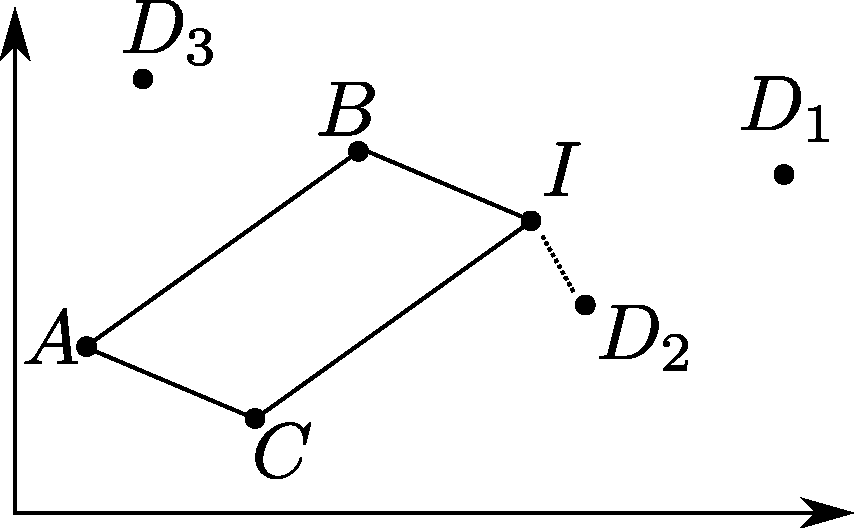
\includegraphics[width=2.5in]{figures/rumelhart_model.pdf}
  \caption{Analogical equation solving process as in \cite{RumAbr73}. The
  solution is here $D_2$.}
\label{FIG:rumelhart_model}
\end{figure}

It is clear that this view of the analogical reasoning process is exactly what
is practically implemented in the experiments of \cite{BayMicDelIJCAI07}, and
all the more so in ours.\todo{ref avant après?}

\paragraph{The Copycat program\\}

Copycat \cite{Mit93} (see also \cite{HofMit94}) is another famous program that
performs analogical reasoning tasks, introduced by Melanie Mitchell and Douglas
Hofstadter. The problems considered by Copycat are the solving of analogical
equations in a \textit{microworld} of strings of letters. A typical Copycat
problem looks as follows: $$\mathbf{abc} : \mathbf{abd} :: \mathbf{ijk} : x$$

What should the value of $x$ be? Various answers may be relevent here, such as
$\mathbf{ijd}$ (replace the right-most letter by $\mathbf{d}$), but the most
natural answer probably is $\mathbf{ijl}$: replace the right-most letter by its
successor. How about $\mathbf{zrq}$? Well, not really convincing. The point of
the authors, however, is that \textit{a priori} every single option should be
given equal chances of success.

This principle is strongly reflected in the Copycat program which is
probabilistic in nature: for the same problem, various solutions can be found
depending on the initial condition. For example the  equation $\mathbf{abd} :
\mathbf{abd} :: \mathbf{mrrjjj} : x$ leads to $\mathbf{mrrkkk}$ in 70\% of the
cases (over 1000 experiments), and to $\mathbf{mrjjk}$ 20\% of the time. Other
less plausible solutions make up the remaining 10\%.

At the beginning of the program, each option is equally available.  Then, on
the basis of their validity, some hypotheses are given a stronger chance to
\textit{survive} till the end of the program, while others are discarded.
Conceptually, this process is emerges from the interoperability of three main
components: the workspace, the codelets, and the temperature.

\begin{itemize}
    \item The workspace, is the place where objects and relations live.
      In the workspace, diverse conceptual structures are built-in:
      \textit{successor}, \textit{predecessor}, \textit{left-most},
      \textit{right-most}, \textit{orientation}, etc. When the program starts, none of these
      structures are activated: this will be the role of the codelets.
    \item The codelets, are competing agents trying to explore and build
      perceptual structures and relations between the objects in the workspace.
      Their behaviour depends on the temparature.
    \item The temperature could be also defined as the entropy of the
      system. When relations in the workspace are strong and well established,
      the temperature is low. At the beginning of the program, the temperature
      is the highest, leading to a multitude of codelets being run in every
      single \textit{direction}. This concept of temperature can be viewed as
      the tradeoff between exploration (trying every possible hypothesis) and
      exploitation (the actual use of a well established hypothesis). When the
      temperature goes below a given threshold, the program stops and the
      current hypothesis is outputed.
\end{itemize}

\begin{figure}[!h]
\centering
  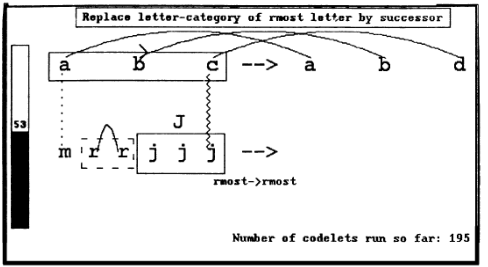
\includegraphics[width=3.5in]{figures/copycat.png}
\caption{Snapshot of Copycat during an equation solving process. Image taken
  from \cite{Mit01}.}
\label{FIG:copycat_snapshot}
\end{figure}

Figure \ref{FIG:copycat_snapshot} illustrate the internal state of Copycat
during the solving of $\mathbf{abc} : \mathbf{abd} :: \mathbf{mrrjjj}: x$. 195
codelets have run so far, so the temperature is average and some structure have
been properly established, such as the \textit{successor group} $\mathbf{abc}$
and the \textit{sameness group} $\mathbf{jjj}$. The $\mathbf{rr}$ group is also
begin defined, though still weaker than the others at this stage. Also, a rule
describing the change from $\mathbf{abc}$ to $\mathbf{abd}$ has been
established: \textit{replace the right-most letter by its successor}. Depending
on the future behaviour of the codelets, this rule with either stick till the
end of the program or change to lead to the most common prediction $x =
\mathbf{kkk}$.

Copycat is clearly a complex adaptative system where a global behaviour emerges
from small, independent parts. According to its authors, \textit{Copycat's
architecture is neither symbolic nor connectionist, nor a hybrid of the two;
rather, the program has a novel type of architecture situated somewhere in
between these extremes}.

\subsection{Analogy and the Minimum Description Length Principle}

Ockham's razor (also Occam), due to the Franciscan philosopher William
of Ockham (1285~-~1347), is a well known principle in machine learning theory.
The main and most useful interpretation of the original latin version states
that when trying to explain a situation, if two hypothesis give the same answer
then the best one is probably the \textbf{simplest} one. In practice, what
makes an hypothesis simple remains quite vague, at least from a computational
point of view. Yet this principle has been formalized into Rissanen's Minimum
Description Length Principle (MDLP) \cite{Ris78}, which is based on Kolmogorov
complexity. Despite the difficulty to build inferential models from this
principle (Kolmogorov complexity is often intractable and impossible to
compute or even to estimate), it has shown to be quite influential in the field
of machine learning, at least from a theoretical point of view.

With this in mind, Antoine Cornuéjols proposed a framework for assessing the
quality of an analogy \cite{CorMLS96} (see also \cite{CorJFA96}). In these
papers, Cornuéjols hypothesizes that the best analogy between a source and a
target model is the one that minimizes its description length, in terms of
Kolmogorov complexity.

Let us first first recall some basic knowledge about Kolmogorov complexity,
before diving into more technical details. The Kolmogorov complexity of a
string of characters $x$, denoted $K(x)$, is the length of the shortest
computer program capable of outputing $x$. $K(x)$ is supposed to capture the
intrinsic complexity of $x$. Intuitively, $K('aaaaabbbbb')$ is supposed to be
lower than $K('abaabbabab')$, because a clear pattern emmerges in the first
string, leading to a simple program: first print $a$ five times, then do the
same for $b$. The second string seems more or less random, which makes it
difficult to factorize into a concize program. In somse sense, the Kolmogorov
complexity captures how well can a string $x$ be \textit{compressed}. The
conditional complexity $K(x \given y)$ is the size of the shortest program that
outputs $x$ when given $y$ as an input.

Now, let's get back to our analogical concerns. As illustrated in figure
\ref{FIG:cornuejols_model}, Cornuéjols considers an analogy as a process
involving an object $x_S$ in a source domain, an object $x_T$ in a target
domain, and two functions $f_S$ and $f_T$ transforming $x_S$ and $x_T$ into
$y_S$ and $y_T$ respectively: $y_S = f_S(x_S)$ and $y_T = f_T(x_T)$. Each
domain $S$ and $T$ \textit{lives} inside a theory or model (namely $M_S$ and
$M_T$), that can describe their corresponding objects.

\begin{figure}[!h]
\centering
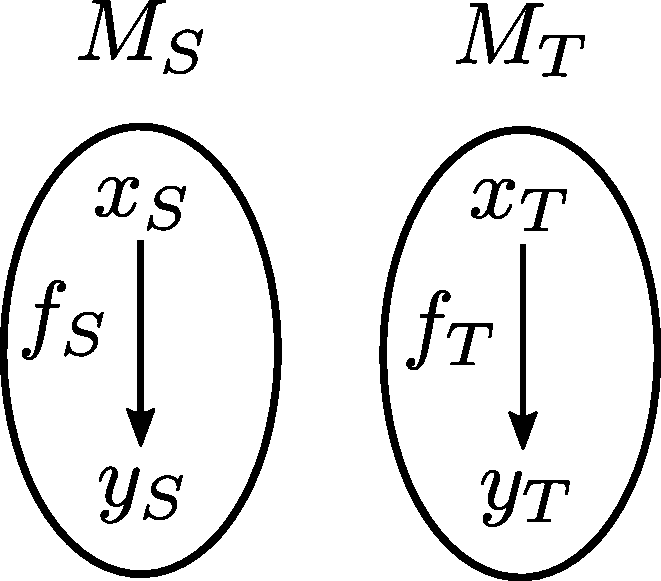
\includegraphics[width=1.5in]{figures/cornuejols_model.pdf}
\caption{The two domains $S$ and $T$ in Cornuejols' model.}
\label{FIG:cornuejols_model}
\end{figure}

For Cornuéjols, the best analogy is the one that minimizes the following sum of
Kolmogorov complexities:
$$K(M_S) + K(x_S \given M_S) + K(f_S \given M_S) + K(M_T \given M_S) + K(x_T
\given M_T) + K(f_T \given M_T),$$
where:
\begin{itemize}
   \item $K(M_S)$ is the cost associated with the source theory,
   \item $K(x_S \given M_S)$ is the cost of $x_S$ as described in the source
     theory,
   \item $K(f_S \given M_S)$ is the cost of $f_S$ as described in the source
     theory,
   \item $K(M_T \given M_S)$ is the cost of describing the target theory from
     the source theory,
   \item $K(x_T \given M_T)$ is the cost of $x_T$ as described in the target
     theory,
   \item and finally $K(f_T \given M_T)$ is the cost of $f_T$ as described in
     the target theory.
\end{itemize}

Notice that the terms $y_i$ are not considered in this cost function, because
they are entirely defined by their corresponding $x_i$ and $f_i$.

Cornuéjols illustrate the plausibility of his model using experiments in the
microworld of Copycat. After defining the Kolmogorov complexity of the built-in
relations (\textit{direction}, \textit{length}, etc.), and those of the
representations of the inputs, the solutions of the analogical equations are
set as those minimizing the above criteria. The empirical results show that
this model, in addition to its theoretical appeal due to the proximity with
MDLP, is at the very least an interesting option to further investigate. In a
recent work , this model of analogy has been applied to a task of transfer
learning \cite{CorMur16}.\todo{Faire lien entre ça et AD de Miclet}

\paragraph{Evans' program to solve geometric problems\\}

The ANALOGY program of Thomas Evans \cite{Eva64} is one of the pioneer work in
the design of programs capable of analogical reasoning. ANALOGY, written in
LISP\footnote{And according to its author, the largest LISP program at the
time!}, is able to solve analogical equations in the form of geometrical
problems, such as that of Figure \ref{FIG:evans}: given three geometrical
patterns, choose the fourth among a list of candidates that leads to the best
proportion.

\begin{figure}[!h]
\centering
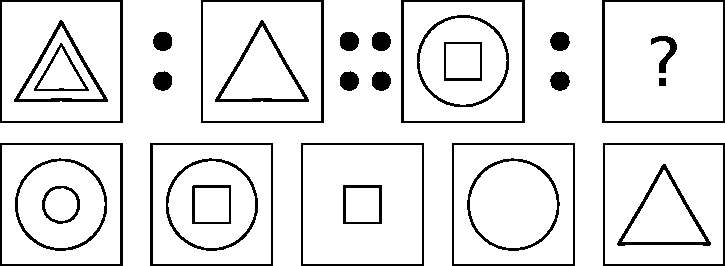
\includegraphics[width=3in]{figures/evans.pdf}
\caption{A geometrical analogy problem}
\label{FIG:evans}
\end{figure}

The inputs to the program are rough, hand-built low-level descriptions of the
figures. For example, simple geometric shape such as circles, rectangles or
triangles are all described with one single primitive:
\textit{SIMPLE\_CLOSED\_CURVE(\dots)}, where the arguments are the start and
end of of the (multiple) lines, and their curvatures. The program is then
devided into two distinct parts.

The role of the first part is to build high level representations of the
figures from these raw descriptions. After identifying coherent shapes (such as
triangle, square, etc) as independent objects, the program tries to find
relations of the kind \textit{INSIDE(Obj1, Obj2)} or \textit{ABOVE(Obj1, Obj3)}
between figures. Finally, similarities between every pair of objects are
computed. The similarity measure is based on the transformability of the first
object into the second one, using tradictional geometrical transformations
(rotation, scale, reflections, etc.). All the information computed by the first
part are given as input (on punched cards!) to the second part.

The second part relates to the analogical solving process per se. Using the
output of the first part, ANALOGY will try to find a set of rules that
transform figure $A$ into figure $B$. A rule would for example state
\textit{REMOVE(Obj1), ROTATE(Obj2, 45\degree), etc.}. Then, by generalizing
each rule, it tries to establish a correspondance between these rules and those
transforming $C$ into one of the candidate solutions. The chosen solution is
that maximizes the resemblance between the two sets of rules.

An interesting fact is that ANALOGY analyses the way to go from $A$ to $B$ and
applies to go from $C$ to $D$, but it does not make use of \textit{central
permutation}: it may just as well analyse the way to go from $A$ to $C$ and
transpose it to go from $B$ to $D$. Note also that in ANALOGY the semantics
behind the relations and the geometrical objects are not taken into account. In
this respect, ANALOGY is close to Gentner's Structure Mapping Theory (and
preexistent by far).

\section{Formal analogical proportions}

An analogical proportion is a statement of the form ``$a$ is to $b$ as $c$ is
to $d$'' involving analogical relations between the pairs $(a,b)$ and $(c,d)$,
as well as between the pairs $(a,c)$ and $(b,d)$.  There are numerous examples
of such statements, with which everybody will more or less agree, such as  ``a
calf is to a cow as a foal is to a mare'', or ``Paris is to France as Berlin is
to Germany''. However, it is only rather recently that formal definitions have
been proposed for analogical proportions in different settings that we briefly
review here.

It has been agreed since Aristotle time that an analogical proportion $A$ is a
quaternary relation satisfying the three following axioms:

\begin{enumerate}
\item $A(a,b,a,b)$ (reflexivity)
\item $A(a,b,c,d) \implies A(c,d,a,b)$ (symmetry)
\item $A(a,b,c,d) \implies A(a,c,b,d)$ (central permutation)
\end{enumerate}

When there is no ambiguity over $A$ and its domain, the infix notation
$a:b::c:d$ is often used.  Considering again our farm example, the symmetry
axiom states that if a calf is to a caw as a foal is to a mare, then a foal is
to a mare as a calf is to a horse, which seems perfectly sound. The central
permutation axiom leads to the natural consequence that a calf is to a foal as
a cow is to a mare.

Starting from the assertion $A(a, b, c, d)$ and by successive application of
the symmetry and central permutation axiom, we arrive to the following eight
equivalent forms:
\begin{align*}
  &A(a, b, c, d)\\
  &A(c, d, a, b)\\
  &A(c, a, d, b)\\
  &A(d, b, c, a)\\
  &A(d, c, b, a)\\
  &A(b, a, d, c)\\
  &A(b, d, a, c)\\
  &A(a, c, b, d)
\end{align*}

Note now that there are exactly $4! = 24$ different orderings of $a, b, c, d$.
We have just seen that $8$ of them form the above equivalence class. There are
two other equivalence classes (each of $8$ orderings, naturally). The first one
is \textit{generated} by $A(a, b, d, c)$ and the second one by $A(a, c, d, b)$.
These theoretical aspects, admittedly tiresome, will however prove useful in
later investigations (Section \ref{Laref}).

There are various models of analogical proportions, depending on the target
domain. We will next review some definitions of analogies in settings that are
of interest for us, but let us first note the following major fact:

\begin{proposition}
  \label{PROPOS:analogy_for_vectors}
  Let $A$ be an analogy over a set $X$. We can define an analogy $A^m$
  over $X^m$ in a component-wise fashion by:
  $$A^m(\mathbf{a}, \mathbf{b}, \mathbf{c}, \mathbf{d}) ~ \emph{  if  } ~
  A(a_i, b_i, c_i, d_i) \emph{ for all } i \in [1, m].$$
\end{proposition}
\noindent
More often than not, $A^m$ will be denoted $A$ for the sake of brevity.

Probably the first use of formal proportions is that of Lepage in
\cite{Lep04} who, starting from the three aforementioned axioms, formally
defined analogical proportions over alphabets of letters with the aim of
generating (analogical) formal languages. His definition have later been
generalized in the works of Stroppa and Yvon (see \cite{StrYvoCNLL05} and
\cite{StrYvoREPORT05})\footnote{In the same work, Stroppa and Yvon also laid
the foundations of analogical learning as used in this thesis (see Section
\ref{la section})}, who provided an algebraic factorization-based definition of
analogical proportions in semigroups:

\begin{definition}
\label{DEF:proportion_semi_group}
Let $(U, \oplus)$ be a semigroup, i.e. $U$ is a set and $\oplus$ is an
  associative binary operation. Four elements $a, b, c, d \in U$, are in proportion if
  there exist some factorization
  \begin{align*}
    a &= a_1 \oplus a_2 \oplus \cdots \oplus a_n\\
    b &= b_1 \oplus b_2 \oplus \cdots \oplus b_n\\
    c &= c_1 \oplus c_2 \oplus \cdots \oplus c_n\\
    d &= d_1 \oplus d_2 \oplus \cdots \oplus d_n,
  \end{align*}

  such that for all $i \in [1, n]$, 
  $$
  \begin{cases}
    a_i = b_i \emph{ and } c_i = d_i\\
    \emph{or}\\
    a_i = c_i \emph{ and } b_i = d_i.
  \end{cases}
  $$
\end{definition}

It will be insighful to instanciate $U$ as the set of natural number
$\mathbb{N}$ and $\oplus$ as the usual multiplication $\times$. In this setting, let's
consider the prime factorization of:

\begin{align*}
  a &= 30 = 1 \times 2 \times 3 \times 5\\
  b &= 60 = 2 \times 2 \times 3 \times 5\\
  c &= 25 = 1 \times 1 \times 5 \times 5\\
  d &= 50 = 2 \times 1 \times 5 \times 5
\end{align*}

For each $i$, we either have $a_i = b_i$ and $c_i = d_i$ ($i = 2, 3, 4$) or
$a_i = c_i$ and $b_i = d_i$ ($i = 1, 4$). We can then say that $a, b, c, d$ are
in proportion, i.e. $30: 60 :: 25:50$. We recognize here the classical
\textbf{geometric proportion}, which states an equality of \textbf{ratios}:
\begin{definition}
\label{DEF:geometric_proportion}
Four real numbers $a, b, c, d$ are in geometric proportion if
$\frac{a}{b} = \frac{c}{d}$, or equivalently if $a\times d = b \times c$.
\end{definition}

It should now be clear for the reader why analogical proportions are
effectively called \textbf{proportions}: it's precisely because they generalize
the well-known numerical (geometric) proportion to other more complex
structures.

Note that the geometric proportion is not the only analogical proportion that
deals with numbers! Indeed, in sections \ref{TODO} we will make use of
the \textbf{arithmetic} proportion, which states an equality of
\textbf{differences}:
\begin{definition}
\label{DEF:arithmetic_proportion}
Four real numbers $a, b, c, d$ are in geometric proportion if $a - b = c - d$.
\end{definition}

Using Proposition \ref{PROPOS:analogy_for_vectors}, four vectors $\mathbf{a},
\mathbf{b}, \mathbf{c}, \mathbf{d}$ of $\mathbb{R}^m$ are in arithmetic
proportion if $\mathbf{a} - \mathbf{b} = \mathbf{c} - \mathbf{d}$, i.e. if they
are the four vertices of a parallelogram, as illustrated in Figure
\ref{FIG:arithmetic_proportion}.

\begin{figure}[!h]
\centering
  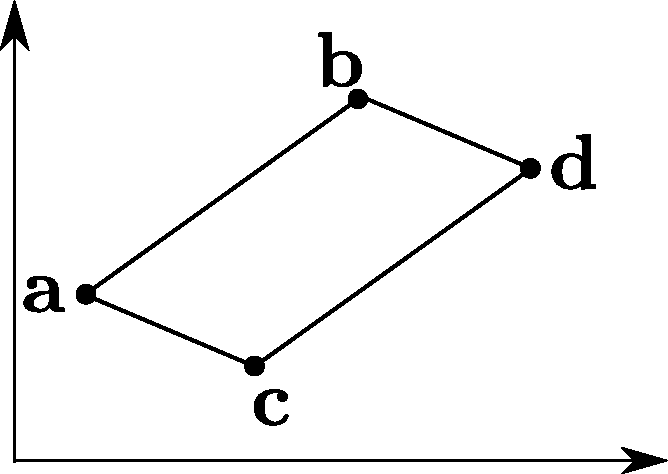
\includegraphics[width=2.5in]{figures/arithmetic_proportion.pdf}
  \caption{$\mathbf{a}, \mathbf{b}, \mathbf{c}, \mathbf{d}$
  are in arithmetic proportion if they are the four vertices of a
  parallelogram.}
\label{FIG:arithmetic_proportion}
\end{figure}

Even if they did not state it in these terms, Rumelhart and Abrahamsen (Section
\ref{TODO}) clearly used the arithmetic proportion for their model of
analogical reasoning.

Beside the use of arithmetic proportion, one of the main focus of this thesis
is to study that of Boolean proportions, i.e.  proportions than one can built
from elements of the set $\mathbb{B} = {0, 1}$. Before diving in more details
into the Boolean proportions, let's first consider the general definition of
analogy in a set, primarly elaborated in \cite{Lep03} as follows: four subsets
$A, B, C, D$ of a universal set $X$ are in proportion if $A$ can be transformed
into $B$ by addind and deleting the same elements as to transform $C$ into $D$.
A more formal definition have been given in \cite{StrYvoREPORT05}:

\begin{definition}
  \label{DEF:analogy_set_facto}
  Let $A, B, C, D \subset X$. $A, B, C, D$ are in proportion if there exists
  four subsets $U, V, W$ and $Z$ (not necessarily disjoint) such that:
  $$
  \begin{cases}
    A = U \cup V\\
    B = U \cup W\\
    C = Z \cup V\\
    D = Z \cup W\\
  \end{cases}
  $$
\end{definition}

To go from $A$ to $B$, one needs to add $W$ and remove $V$. To go from $C$ to
$D$, one needs to do the exact same thing: add $W$ and remove $V$. An
equivalent definition has been given in \cite{MicPra09}:

\begin{definition}
  \label{DEF:analogy_set_miclet_henri}
  Let $A, B, C, D \subset X$. $A, B, C, D$ are in proportion if:
  $$
  A \setminus B = C \setminus D \emph{ and } B \setminus A = D \setminus A
  $$
\end{definition}

Definition \ref{DEF:analogy_set_miclet_henri} reads as \textit{$A$ differs from
$B$ as $C$ differs from $D$, and $B$ differs from $A$ as $D$ differs from $C$},
which is naturally equivalent to the statement of Definition
\ref{DEF:analogy_set_facto}: $A \setminus B = C \setminus D = V$, and $B
\setminus A = D \setminus A  = W$. The formula of Definition
\ref{DEF:analogy_set_miclet_henri} is actually equivalent to the following form
(not without using various ingenious tweaks): $$A \cup D = B \cup C \text{ and
} A \cap D = B \cap C.$$

As an example, let's consider $A = \{a, b, c, g\}, B = \{a, b, d, e, g\}, C =
\{c, f, g\}$ and $D = \{d, e, f, g\}$, as summed-up in Table
\ref{TAB:analogy_sets}.

\begin{table}[h!]
\centering
$$
\begin{tabular}{| c | c  c  c  c  c  c  c |}
\toprule
  & a & b & c & d & e & f & g\\
\midrule
  A & \times & \times & \times &  &  &  & \times \\
  B & \times & \times &  & \times & \times &  & \times\\
  C &  &  & \times &  &  & \times & \times\\
  D &  &  &  & \times & \times & \times & \times\\
\bottomrule
\end{tabular}
$$
\caption{Four sets $A, B, C, D$ in analogical proportion.}
\label{TAB:analogy_sets}
\end{table}

Setting $U = \{a, b, g\}, V = \{c\}, W = \{d, e\}$ and $Z = \{f, g\}$, the
conditions of Definition  \ref{DEF:analogy_set_facto}  are clearly satisfied.
Also, $A \setminus B = C \setminus D = \{c\} = V$, and $B\setminus A = D
\setminus C = \{d, e\} = W$. Finally, $A \cup D = B \cup C = \{a, b, c, d, e,
f, g\}$ and $A\cap D = B\cap C = \{g\}$.

We can also recognize in Table \ref{TAB:analogy_sets} that the conditions of
Definition \ref{DEF:proportion_semi_group} are satisfied, i.e. for all $i$ we
have either $A_i = B_i$ and $C_i = D_i$, or $A_i = C_i$ and $B_i = D_i$. As we
will now see, these two patterns are at the core of the Boolean analogical
proportions, whose definition directly comes from Definition
\ref{DEF:analogy_set_miclet_henri} and by considering the set $\{0, 1\}$:

\begin{definition}
  \label{DEF:boolean_proportion}
  Four elements $a, b, c, d$ in $\mathbb{B} = \{0, 1\}$ are in proportion if
  \begin{alignat*}{2}
    &(a \leftrightarrow b \wedge c \leftrightarrow d) && \vee (a
    \leftrightarrow c \wedge b \leftrightarrow d), \emph{ or equivalently}\\
     & (a \wedge d \leftrightarrow b \wedge c) &&\wedge (a \vee  d
    \leftrightarrow b \vee c),
  \end{alignat*}
  where $\leftrightarrow$ stands for the equivalence connective.
\end{definition}

\todo{Dire qu'il y a plein d'autres modèles, celui la n'est que le minimal}
These scary formulas state the exact same facts as the previous definition,
i.e. that $a$ differs from $b$ as $c$ differs from $d$ and conversely $b$
differs from $a$ as $d$ differs from $c$. Again, an equivalent definition is
that $a, b, c, d$ are in proportion if $a = b$ and $c = d$, or $a = c$ and $b =
d$.

In a Boolean setting, there are exactly $2^4 = 16$ different valuations of $a,
b, c, d$. The only $6$ valuations (or \textbf{patterns}) that lead to a valid
Boolean proportion are illustrated in Table \ref{TAB:six_valid_patterns}.

\begin{table}[t]
  \centering
  $$
  \begin{array}{|cccc|c|}
    \toprule
    a & b & c & d &  A(a, b, c, d)\\
    \midrule
    0 & 0 & 0 & 0 &   \textbf{1}\\
    1 & 1 & 1 & 1 &   \textbf{1}\\
    0 & 0 & 1 & 1 &   \textbf{1}\\
    1 & 1 & 0 & 0 &   \textbf{1}\\
    0 & 1 & 0 & 1 &   \textbf{1}\\
    1 & 0 & 1 & 0 &   \textbf{1}\\
    \bottomrule
  \end{array}
  $$
  \caption{The six valid patterns of the Boolean proportion.}
  \label{TAB:six_valid_patterns}
\end{table}

Table \ref{TAB:six_valid_patterns} provides us with valuable insights. First,
note that some sort of {\it code independence axiom} is satisfied, which
guarantees that $0$ and $1$ play symmetric roles:

\begin{property}
  Let a, b, c, d in $\mathbb{B}$. Then  $a : b :: c : d \iff \neg a :  \neg
  b ::  \neg c :  \neg d.$
\end{property}

Also, it appears that the Boolean proportion is equivalent to the arithmetic
proportion when we restrict it to $\mathbb{B}$:

\begin{property}
  Let a, b, c, d in $\mathbb{B}$. Then  $a : b :: c : d \iff a - b = c - d$.\\
  Note that the geometric proportion offers a necessary condition, but not a
  sufficient one: $a \times d = b\times c$ is satisfied by all of the patterns
  in Table \ref{TAB:six_valid_patterns}, but also for the pattern $0: 0: 0: 1$
  which is not a valid analogy.
\end{property}

Just like in $\mathbb{R}^m$, the arithmetic proportion allows us to think of
Boolean proportions as (potentially \textit{flat}) parallelograms, but this
time we are restricted to $\mathbb{B}^m$. Figure \ref{FIG:proportions_in_B2}
illustrates the proportions that one can build in $\mathbb{B}^2$:
\begin{itemize}
  \item the proportion $\mathbf{a}: \mathbf{b} :: \mathbf{c} : \mathbf{d}$ and
    its 7 other equivalent forms, forming the parallelogram
    $\mathbf{a}\mathbf{b}\mathbf{c}\mathbf{d}$ ;
  \item the proportions that we can build using any pair of vertices, for
    example $\mathbf{a} : \mathbf{d} :: \mathbf{a} : \mathbf{d}$. Each of these
    proportions has three other equivalent forms: in our case $\mathbf{a} :
    \mathbf{a} :: \mathbf{d} : \mathbf{d}$, $\mathbf{d} : \mathbf{a} ::
    \mathbf{d} : \mathbf{a}$ and $\mathbf{d} : \mathbf{d} :: \mathbf{a} :
    \mathbf{a}$ ;
  \item the four proportions involving each vertex independently, for example
    $\mathbf{b}:\mathbf{b}::\mathbf{b}:\mathbf{b}$.
\end{itemize}

\begin{figure}[!h]
\centering
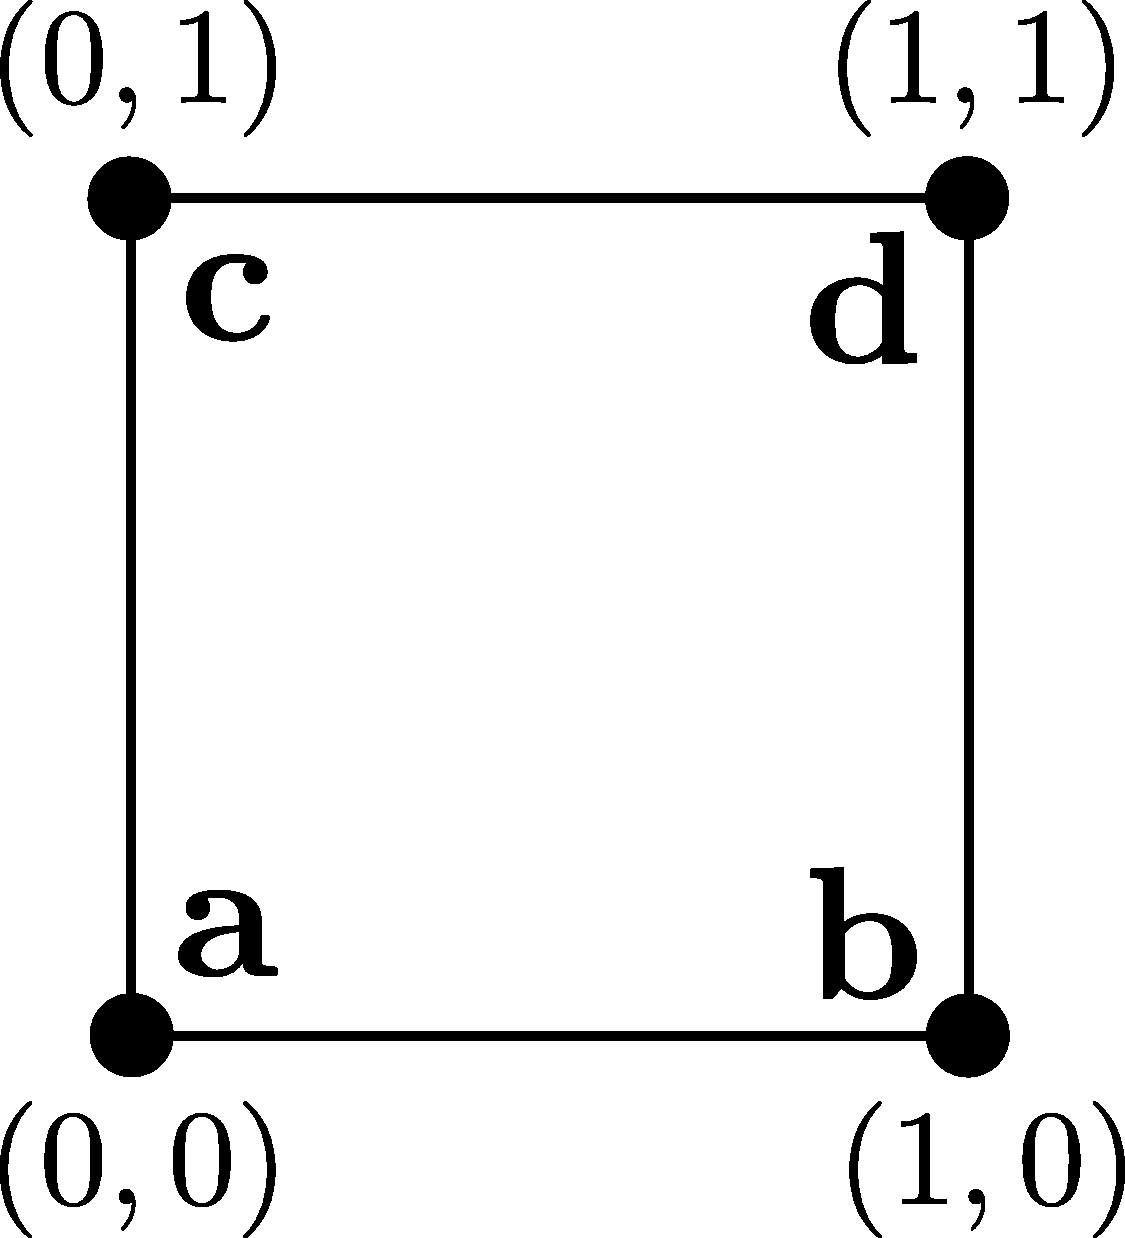
\includegraphics[width=1.5in]{figures/proportions_in_B2.pdf}
  \caption{Proportions in $\mathbb{B}^2$}
\label{FIG:proportions_in_B2}
\end{figure}

All in all, this makes up to $36 = 8 + 6 \times 4 + 4$ proportions, but only $1
+ 6 + 4 = 11$ of them can be considered \textit{unique} (up to equivalence) and
only one is non-flat\footnote{\textit{flat} proportion are those that make up
flat parallelograms. This naming convention is actually fortunate, because
these proportion are in practice absolutely useless.}. In section \ref{TODO},
we will further investigate the number of unique proportions that can be built
in $\mathbb{B}^m$.

Going a dimension further can still be insightful. Figure \ref{FIG:cubes_in_B3}
illustrates the 12 non-flat proportions that exist in $\mathbb{B}^3$. These
proportions are the paralellograms making up the 6 faces of the $3$-cube, and
six other \textit{diagnoal} parallelograms. The flat proportions are not (all)
shown for obvious reasons.

\begin{figure}[!h]
\centering
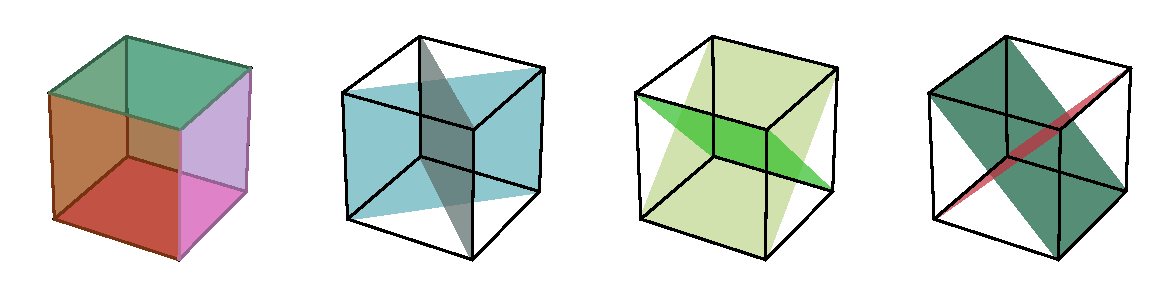
\includegraphics[width=\linewidth]{figures/cubes_in_B3.pdf}
  \caption{The twelve \textit{non-flat} parallelograms in $\mathbb{B}^3$}
\label{FIG:cubes_in_B3}
\end{figure}

\paragraph{Machine learning with Boolean proportions\\}

We now have enough backgroud on Boolean proportions to start doing some machine
learning. Here is our problem. We consider the set $\mathbb{B}^m$ and its $2^m$
elements. For various $\mathbf{x} \in \mathbb{B}^m$, we know the value of
$f(\mathbf{x})$, where $f$ is a function from $\mathbb{B}^m$ to $\mathbb{B}$.
The value $f(\mathbf{x})$ is called the \textbf{class} of $\mathbf{x}$, or its
\textbf{label}. The set $S \subsetneq \mathbb{B}^m$ of elements for which
$f(\mathbf{x})$ is known is called the \textbf{training set}. For any element
$\mathbf{x} \notin S$, $f(\mathbf{x})$ is unknown and our goal is to guess it:
this is a \textbf{classification problem}.

Suppose we're in $\mathbb{B}^3$ and consider Figure
\ref{FIG:classification_problem}.
\begin{figure}[!h]
\centering
  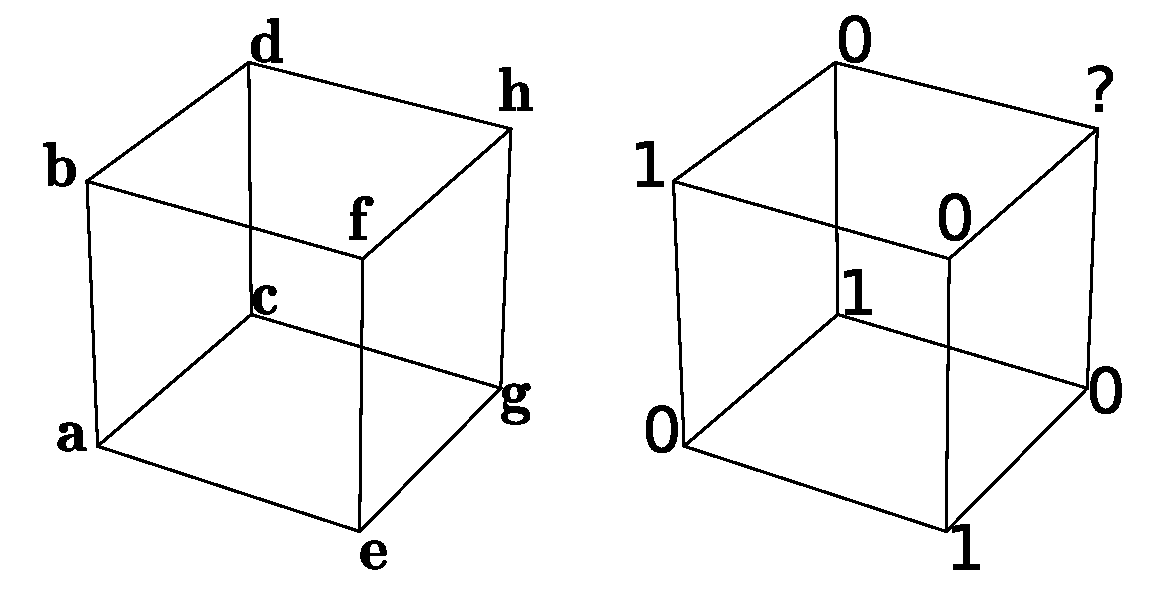
\includegraphics[width=3in]{figures/classification_problem.pdf}
  \caption{What should the value of $f(\mathbf{h})$ be?}
\label{FIG:classification_problem}
\end{figure}
We know the values of $f(\mathbf{x})$ for
every single $\mathbf{x}$ but $\mathbf{h}$, so $S = \{ \mathbf{a}, \mathbf{b},
\mathbf{c}, \mathbf{d}, \mathbf{e}, \mathbf{f}, \mathbf{g}\}$. To guess the value of
$f(\mathbf{h})$, we will use the so-called analogical inference principle,
which states that if four elements $\mathbf{a}, \mathbf{b}, \mathbf{c},
\mathbf{d}$ are in proportion, then their class should also be in proportion:
$$
\infer{f(\mathbf{a}) : f(\mathbf{b}) :: f(\mathbf{c})
: f(\mathbf{d})}{\mathbf{a} : \mathbf{b} :: \mathbf{c} : \mathbf{d}}
$$

This is obviously an unsound principle, in that the conclusion does not
logically follows from the premice. But as we will see in this document, it can
still be useful.

This principle leads us to look for all 3-tuples $(\mathbf{x}, \mathbf{y},
\mathbf{z}) \in S^3$ such that $\mathbf{x}:\mathbf{y}::\mathbf{z}:\mathbf{h}$.
The analogical inference then states that we should have
$f(\mathbf{x}):f(\mathbf{y})::f(\mathbf{z}):f(\mathbf{h})$. Figure
\ref{FIG:cubes_in_B3} tells us that there are 6 (non-flat) parallelograms
involving $\mathbf{h}$ as a vertex. The six corresponding proportions are:

\begin{itemize}
  \item $\mathbf{b} : \mathbf{d} :: \mathbf{f} : \mathbf{h}$
  \item $\mathbf{e} : \mathbf{f} :: \mathbf{g} : \mathbf{h}$
  \item $\mathbf{c} : \mathbf{g} :: \mathbf{d} : \mathbf{h}$
  \item $\mathbf{a} : \mathbf{b} :: \mathbf{g} : \mathbf{h}$
  \item $\mathbf{a} : \mathbf{e} :: \mathbf{d} : \mathbf{h}$
  \item $\mathbf{a} : \mathbf{c} :: \mathbf{f} : \mathbf{h}$
\end{itemize}

Unfortunately, the first three proportion are of no use here. 

Notice that we have light-heartedly ignored  all the flat proportions. This is
because...

\paragraph{How many proportions can we build in $\mathbb{B}^m$?\\}

Exactly $6^m$! And it is fairly easy to derive: there are $6$ proportions in
$\mathbb{B}$. As a proportion in $\mathbb{B}^2$ is the concatenation of any
two propotions in $\mathbb{B}$, there are exactly $6^2 = 36$ proportions in
$\mathbb{B}^2$. Because analogical proportions in $\mathbb{B}^m$ are the
concatenation of $m$ proportions in $\mathbb{B}$ (the proportion is evaluated
component-wise), one can build $6^m$ proportions in $\mathbb{B}^m$.

But let's now ask a more relevent and challenging question: how many
\textit{useful} proportions can we build in $\mathbb{B}^m$? By \textit{useful},
we mean proportions that could be used for classification purposes.

\begin{aquote}{The astute reader, who has been struck by divine light}
  What a silly question! There are obviously $\frac{6^m}{8} - 4^{m - 1} + 2^{m
  - 3}$ such proportions! How can you not be aware of the A016283 sequence from
  the OEIS\footnote{The On-line Encyclopedia of Integer Sequences
  (http://oeis.org/A016283)}?!
\end{aquote}

Unfortunately, we, who have not (yet) been struck by divine light, will have to
derive this formula ourselves. The only proportions
$\mathbf{a} : \mathbf{b} :: \mathbf{c} : \mathbf{d}$ that are useful for
classification purposes are those where all elements $\mathbf{a}, \mathbf{b},
\mathbf{c}, \mathbf{d}$ are distinct.\todo{Expliquer pourquoi selon où on le
met}

We already know that every proportion in $\mathbb{B}^m$ is a parallelogram, and
that there are $6^m$ parallelograms. The geometrical interpretation of the
above statement is that we are here interested only in non-flat parallelgrams,
i.e. parallelograms involving four distinct vertices. We thus want to exclude
from the $6^m$ proportions those that comply with one of the three following
patterns:

\begin{itemize}
  \item $\mathbf{x}: \mathbf{x} :: \mathbf{x} : \mathbf{x}$
  \item $\mathbf{x}: \mathbf{x'} :: \mathbf{x} : \mathbf{x'}$
  \item $\mathbf{x}: \mathbf{x} :: \mathbf{x'} : \mathbf{x'}$
\end{itemize}

Now, let's count them.

\begin{itemize}
  \item Every vertex $\mathbf{a}$ will generate a proportion of the form
    $\mathbf{a}: \mathbf{a} :: \mathbf{a} : \mathbf{a}$, so there are exactly
    $2^m$ proportions $\mathbf{x}: \mathbf{x} :: \mathbf{x} : \mathbf{x}$,.
  \item Every pair $(\mathbf{a}, \mathbf{b})$ of vertices will generate a
    proportion $\mathbf{a}: \mathbf{b} :: \mathbf{a} : \mathbf{b}$, and another
    proportion $\mathbf{b}: \mathbf{a} :: \mathbf{b} : \mathbf{a}$. There are
    $\binom{2^m}{2}$ pairs $(\mathbf{a}, \mathbf{b})$, so in total this makes
    $2\binom{2^m}{2}$ proportions of the form $\mathbf{x}: \mathbf{x'} ::
    \mathbf{x} : \mathbf{x'}$. 
  \item Every pair $(\mathbf{a}, \mathbf{b})$ of vertices will also generate a
    proportion $\mathbf{a}: \mathbf{a} :: \mathbf{b} : \mathbf{b}$, and another
    proportion $\mathbf{b}: \mathbf{b} :: \mathbf{a} : \mathbf{a}$. There are
    thus $2\binom{2^m}{2}$ proportions of the form $\mathbf{x}: \mathbf{x} ::
    \mathbf{x'} : \mathbf{x'}$.
\end{itemize}


\chapter{Formal analogical proportions}
\label{CHAP:formal_analogical_proportions}

\initial{A}fter the long (and somewhat tedious) introduction of past works on
analogical reasoning in Chapter \ref{CHAP:chapter_1}, we here choose a
different and hopefully more engaging approach. Rather than bore (and lose) the
reader with a never-ending list of definitions and properties, we will try to
guide her through an insightful tutorial on the use of Boolean proportions and
their application to a small classification task. This will allow us to
introduce many of the key concepts used in the rest of our work, and to
illustrate their use with concrete examples. Only then will we provide the
complete, formal definitions of analogical proportion in algebraic settings. We
first start by diving into the realm of Boolean proportions.

\section{A shortcut from Aristotle to Boolean proportions}
\label{SEC:shortcut_from_aristotle_to_boolean_proportions}

An \textbf{analogical proportion} is a statement of the form ``$a$ is to $b$ as
$c$ is to $d$'' involving analogical relations between the pairs $(a,b)$ and
$(c,d)$, as well as between the pairs $(a,c)$ and $(b,d)$.  There are numerous
examples of such statements, with which everybody will more or less agree, such
as  ``a calf is to a cow as a foal is to a mare'', or ``Paris is to France as
Berlin is to Germany''.

It has been agreed since Aristotle time that an analogical proportion $A$ is a
quaternary relation satisfying the three following axioms, for any $a, b, c, d$:

\begin{enumerate}
\item $A(a,b,a,b)$ always holds (Reflexivity)
\item $A(a,b,c,d) \implies A(c,d,a,b)$ (Symmetry)
\item $A(a,b,c,d) \implies A(a,c,b,d)$ (Central permutation)
\end{enumerate}

When there is no ambiguity over $A$ and its domain, the infix notation
$a:b::c:d$ is often used. Considering again our farm example, the symmetry
axiom states that if a calf is to a cow as a foal is to a mare, then a foal is
to a mare as a calf is to a cow, which seems perfectly sound. The central
permutation axiom leads to the natural consequence that a calf is to a foal as
a cow is to a mare.
Starting from the assertion $A(a, b, c, d)$ and by successive application of
the symmetry and central permutation axioms, we arrive to the following eight
equivalent forms:
\begin{align*}
       &A(a, b, c, d)\\
  \iff &A(c, d, a, b)\\
  \iff &A(c, a, d, b)\\
  \iff &A(d, b, c, a)\\
  \iff &A(d, c, b, a)\\
  \iff &A(b, a, d, c)\\
  \iff &A(b, d, a, c)\\
  \iff &A(a, c, b, d).
\end{align*}

Note now that there are exactly $4! = 24$ different orderings of $a, b, c, d$.
We have just seen that $8$ of them constitute the above equivalence class.
There are two other equivalence classes (each of $8$ orderings, naturally), for
a total of three equivalence classes. The first one is \textit{generated} by
$A(a, b, c, d)$, the second one by $A(a, b, d, c)$ and the third one by $A(a,
c, d, b)$.

There are various models of analogical proportions, depending on the target
domain. In section \ref{SEC:formal_definitions_proportions}, we will review
some definitions of analogical proportions in settings that are of interest for
us, but let us first focus on the \textbf{Boolean proportion}, i.e. proportions
dealing with Boolean numbers in $\mathbb{B} = \{0, 1\}$. The Boolean proportion
will indeed be one a our main object of study in this thesis.

The first axiom tells us that the proportion $a:b::a:b$ holds for any value of
$a$ and $b$ in $\mathbb{B}$. This means that the four following proportions are
valid:
\begin{itemize}
  \item $0 : 1 :: 0 :1$
  \item $1 : 0 :: 1 :0$
  \item $0 : 0 :: 0 :0$
  \item $1 : 1 :: 1 :1$
\end{itemize}

Using the central permutation axiom, we can derive two additional proportions:

\begin{itemize}
  \item $1 : 1 :: 0 : 0$
  \item $0 : 0 :: 1 : 1$
\end{itemize}

In a Boolean setting, there are exactly $2^4 = 16$ different valuations of $a,
b, c, d$. We have derived so far $6$ valuations (or \textbf{patterns}) that
lead to a valid Boolean proportions, which are summed-up in Table
\ref{TAB:six_valid_patterns}. In Section
\ref{SEC:formal_definitions_proportions}, we will give a more formal definition
of Boolean proportions, indicating that the remaining $10$ patterns all lead to
incorrect proportions, so the only valid ones are those of Table
\ref{TAB:six_valid_patterns}.

\begin{table}[t]
  \centering
  $$
  \begin{array}{ccccc}
    \toprule
    a & b & c & d &  A(a, b, c, d)\\
    \midrule
    0 & 0 & 0 & 0 &   \textbf{1}\\
    1 & 1 & 1 & 1 &   \textbf{1}\\
    0 & 0 & 1 & 1 &   \textbf{1}\\
    1 & 1 & 0 & 0 &   \textbf{1}\\
    0 & 1 & 0 & 1 &   \textbf{1}\\
    1 & 0 & 1 & 0 &   \textbf{1}\\
    \bottomrule
  \end{array}
  $$
  \caption{The six valid patterns of the Boolean proportion.}
  \label{TAB:six_valid_patterns}
\end{table}

Table \ref{TAB:six_valid_patterns} provides us with valuable insights.  First,
it appears that the Boolean proportion can be defined in the following way:

\begin{definition}
  \label{DEF:boolean_proportion_informal}
  Four elements $a, b, c, d$ in $\mathbb{B}$ are in proportion if:
  $$
  \begin{cases}
    a = b \emph{ and } c = d\\
    \emph{or}\\
    a = c \emph{ and } b = d.
  \end{cases}
  $$
\end{definition}

From a numerical point of view, it also appears that $a:b::c:d$ is true if and
only if $a - b = c - d$. A relation $a - b = c - d$ between four elements $a,
b, c, d$ in $\mathbb{R}$ is called an \textbf{arithmetic proportion}.
The arithmetic proportion is a particular instance of analogical proportion,
and it turns out that when restricted to $\mathbb{B}$, it is
\textbf{equivalent} to the Boolean proportion.

The arithmetic proportion, which states an equality of differences, is not the
only proportion that deals with numbers. The \textbf{geometric proportion} is
another instance of analogical proportion, which states an equality of ratios:
four elements $a, b, c, d$ of $\mathbb{R}$ are in geometric proportion if
$\frac{a}{b} = \frac{c}{d}$, or equivalently if $a\times d = c\times b$.
Note that in $\mathbb{B}$ the geometric proportion offers a necessary condition
to define the Boolean proportion, but not a sufficient one: $a \times d =
b\times c$ is satisfied by all of the patterns in Table
\ref{TAB:six_valid_patterns}, but also for the pattern $0: 0: 0: 1$ which is
not a valid analogy.

It should now be clear for the reader why analogical proportions are
effectively called \textbf{proportions}: it's precisely because they generalize
the well-known numerical geometric proportion to more complex structures.
Actually, Aristotle stated the three aforementioned axioms on the basis of the
geometric proportion.

We also note from Table \ref{TAB:six_valid_patterns} that some sort of {\it
code independence axiom} is satisfied, which guarantees that $0$ and $1$ play
symmetric roles:

\begin{property}
  Let a, b, c, d in $\mathbb{B}$. Then
  $$a : b :: c : d \iff \neg a :  \neg b ::  \neg c :  \neg d,$$
  where $\neg x$ is the negation of $x$.
\end{property}

Now, an analogical proportion in $\mathbb{B}$ is great, but what we are
interested in is a proportion in $\mathbb{B}^m$, to be able to deal with
Boolean vectors. A natural extension of the Boolean proportion to
$\mathbb{B}^m$ is to require that each of the $m$ dimensions make up valid
proportions in $\mathbb{B}$:

\begin{definition}
  \label{DEF:analogy_for_vectors}
  Let $A$ be an analogy over a set $X$. We can define an analogy $A^m$
  over $X^m$ in a component-wise fashion by:
  $$A^m(\mathbf{a}, \mathbf{b}, \mathbf{c}, \mathbf{d}) ~ \emph{  if  } ~
  A(a_i, b_i, c_i, d_i) \emph{ for all } i \in [1, m],$$
  where $\mathbf{a}, \mathbf{b}, \mathbf{c}, \mathbf{d}$ are vectors in $X^m$.
\end{definition}
\noindent
More often than not, $A^m$ will simply be denoted $A$ for the sake of brevity.
So far we have seen a proportion in $\mathbb{B}$ and two proportions in
$\mathbb{R}$. Thanks to Definition \ref{DEF:analogy_for_vectors}, we now have
the definition of a proportion in $\mathbb{B}^m$, and two numerical proportions
in $\mathbb{R}^m$. The interpretation of the geometric proportion in
$\mathbb{R}^m$ can be opaque, but that of the arithmetic proportion is very
clear: four vectors $\mathbf{a}, \mathbf{b}, \mathbf{c}, \mathbf{d}$ of
$\mathbb{R}^m$ are in arithmetic proportion if $\mathbf{a} - \mathbf{b} =
\mathbf{c} - \mathbf{d}$, i.e. if they are the four vertices of a
parallelogram, as illustrated in Figure \ref{FIG:arithmetic_proportion}.

\begin{figure}[!h]
\centering
  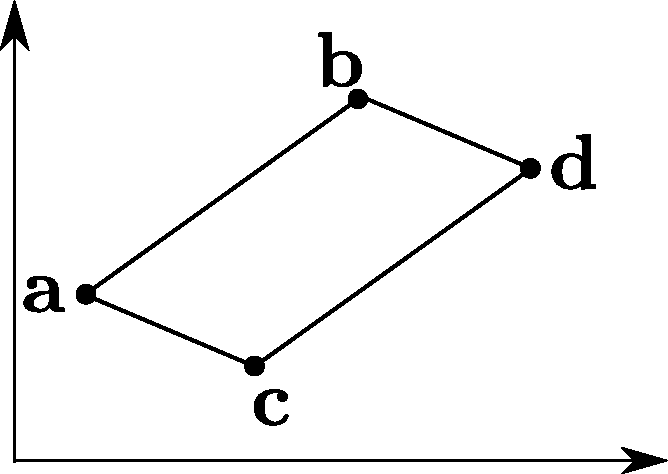
\includegraphics[width=2.5in]{figures/arithmetic_proportion.pdf}
  \caption{$\mathbf{a}, \mathbf{b}, \mathbf{c}, \mathbf{d}$
  are in arithmetic proportion iff they are the four vertices of a
  parallelogram.}
\label{FIG:arithmetic_proportion}
\end{figure}

Even if they did not state it in these terms, Rumelhart and Abrahamsen (Section
\ref{SEC:rumelhart_Abrahamsen}) clearly used the arithmetic proportion for their model of
analogical reasoning.

We have seen that in $\mathbb{B}$, and thus in $\mathbb{B}^m$, the Boolean
proportion and the arithmetic proportion are equivalent. This means that a
proportion in $\mathbb{B}^m$ can also be represented as a (potentially
\textit{flat}) parallelogram.
Figure \ref{FIG:proportions_in_B2} illustrates the proportions that one can
build in $\mathbb{B}^2$:
\begin{itemize}
  \item the proportion $\mathbf{a}: \mathbf{b} :: \mathbf{c} : \mathbf{d}$ and
    its 7 other equivalent forms, making up the parallelogram
    $\mathbf{a}\mathbf{b}\mathbf{c}\mathbf{d}$ ;
  \item the proportions that we can build using any pair of vertices, for
    example $\mathbf{a} : \mathbf{d} :: \mathbf{a} : \mathbf{d}$. Each of these
    proportions has three other equivalent forms: in our case $\mathbf{a} :
    \mathbf{a} :: \mathbf{d} : \mathbf{d}$, $\mathbf{d} : \mathbf{a} ::
    \mathbf{d} : \mathbf{a}$ and $\mathbf{d} : \mathbf{d} :: \mathbf{a} :
    \mathbf{a}$ ;
  \item the four proportions involving each vertex independently, for example
    $\mathbf{b}:\mathbf{b}::\mathbf{b}:\mathbf{b}$.
\end{itemize}

\begin{figure}[!h]
\centering
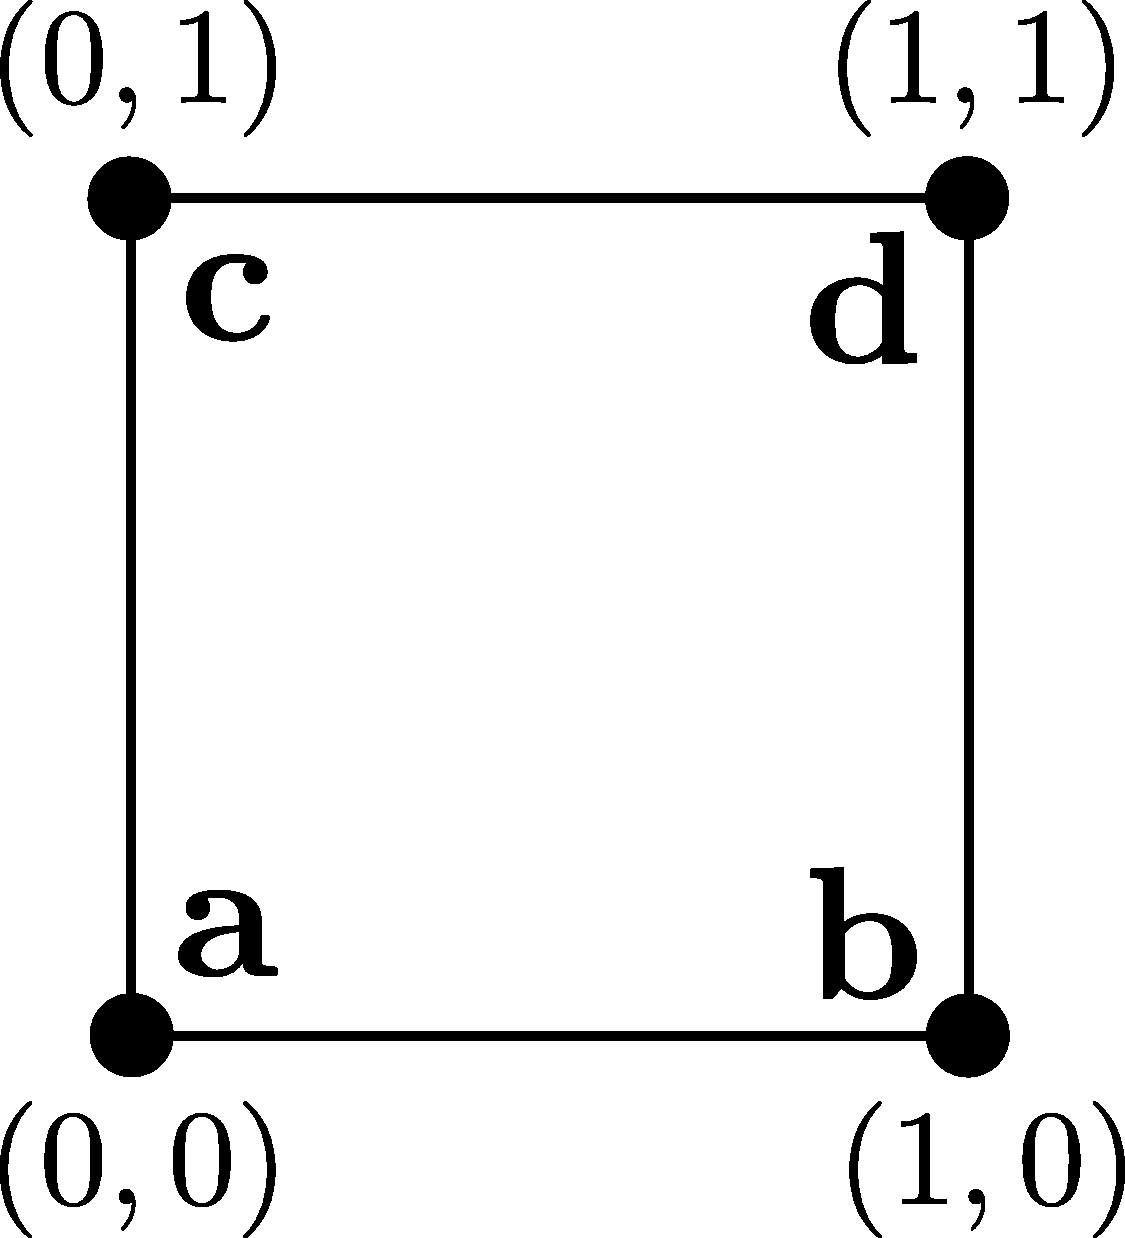
\includegraphics[width=1.5in]{figures/proportions_in_B2.pdf}
  \caption{The $36$ proportions in $\mathbb{B}^2$.}
\label{FIG:proportions_in_B2}
\end{figure}

All in all, this makes up to $36 = 8 + 6 \times 4 + 4$ proportions, but only $1
+ 6 + 4 = 11$ of them can be considered \textit{unique} (up to equivalence) and
only one is non-flat\footnote{\textit{flat} proportion are those that make up
flat parallelograms. This naming convention is actually fortunate, because
these proportion are in practice absolutely useless, as it will soon become
clear.}. In section \ref{SEC:number_of_parallelograms_in_Bm}, we will further
investigate the number of unique proportions that can be built in
$\mathbb{B}^m$.

Going a dimension further can still be insightful. Figure \ref{FIG:cubes_in_B3}
illustrates the 12 non-flat proportions that exist in $\mathbb{B}^3$. These
proportions are the parallelograms making up the 6 faces of the $3$-cube, and
six other \textit{diagonal} parallelograms. The flat proportions are not (all)
shown for the sake of clarity.

\begin{figure}[!h]
\centering
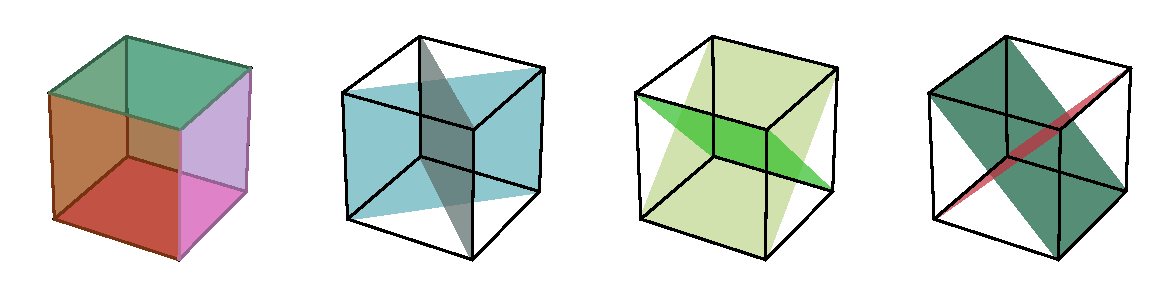
\includegraphics[width=\linewidth]{figures/cubes_in_B3.pdf}
  \caption{The twelve \textit{non-flat} parallelograms in $\mathbb{B}^3$.}
\label{FIG:cubes_in_B3}
\end{figure}

Before applying our fresh knowledge to a classification problem in the next
section, let us first note the following remarkable property, which will be
useful to us much later in Section \ref{TODO}:

\begin{property}
  \label{PROPER:hamming_distance_boolean_proportion}
  Let $\mathbf{a}, \mathbf{b},\mathbf{c}, \mathbf{d}$ in $\mathbb{B}^m$, and
  let $H(\mathbf{x}, \mathbf{x'})$ be the Hamming distance between $\mathbf{x}$
  and $\mathbf{x'}$, i.e. the number of components we need to flip to transform
  $\mathbf{x}$ into $\mathbf{x'}$ (or the reverse).\\
  If $\mathbf{a} : \mathbf{b}
  :: \mathbf{c} : \mathbf{d}$, then these three equalities hold:

  $$
  \begin{cases}
    H(\mathbf{a}, \mathbf{b}) = H(\mathbf{c}, \mathbf{d})\\
    H(\mathbf{a}, \mathbf{c}) = H(\mathbf{b}, \mathbf{d})\\
    H(\mathbf{a}, \mathbf{d}) = H(\mathbf{b}, \mathbf{c}).
  \end{cases}
  $$
\end{property}

We can easily verify this property in $\mathbb{B}$ from Table
\ref{TAB:six_valid_patterns}. The general case in $\mathbb{B}^m$ immediately
follows from Definition \ref{DEF:analogy_for_vectors}. Sadly, Property
\ref{PROPER:hamming_distance_boolean_proportion} only offers a necessary
condition for a proportion to hold, and not a sufficient one. We note that
while the first two properties $H(\mathbf{a}, \mathbf{b}) = H(\mathbf{c},
\mathbf{d})$ and $H(\mathbf{a}, \mathbf{c}) = H(\mathbf{b}, \mathbf{d})$ are
classical properties for parallelograms, the third one $H(\mathbf{a},
\mathbf{d}) = H(\mathbf{b}, \mathbf{c})$ is only true for rectangles. In fact,
the parallelograms that we can build in $\mathbb{B}^m$ are always rectangles.

\section{Machine learning with Boolean proportions: a quick walk-through}
\label{SEC:machine_learning_with_boolean_proportions}

We now have enough background on Boolean proportions to start doing some machine
learning. Here is our problem. We consider the set $\mathbb{B}^m$ and its $2^m$
elements. For various $\mathbf{x} \in \mathbb{B}^m$, we know the value of
$f(\mathbf{x})$, where $f$ is a function from $\mathbb{B}^m$ to $\mathbb{B}$.
The value $f(\mathbf{x})$ is called the \textbf{class} of $\mathbf{x}$, or its
\textbf{label}. The set $S \subsetneq \mathbb{B}^m$ of elements for which
$f(\mathbf{x})$ is known is called the \textbf{training set}. For any element
$\mathbf{x} \notin S$, $f(\mathbf{x})$ is unknown and our goal is to guess it:
this is a binary \textbf{classification problem}.

Suppose we're in $\mathbb{B}^3$ and consider Figure
\ref{FIG:classification_problem}.
\begin{figure}[!h]
\centering
  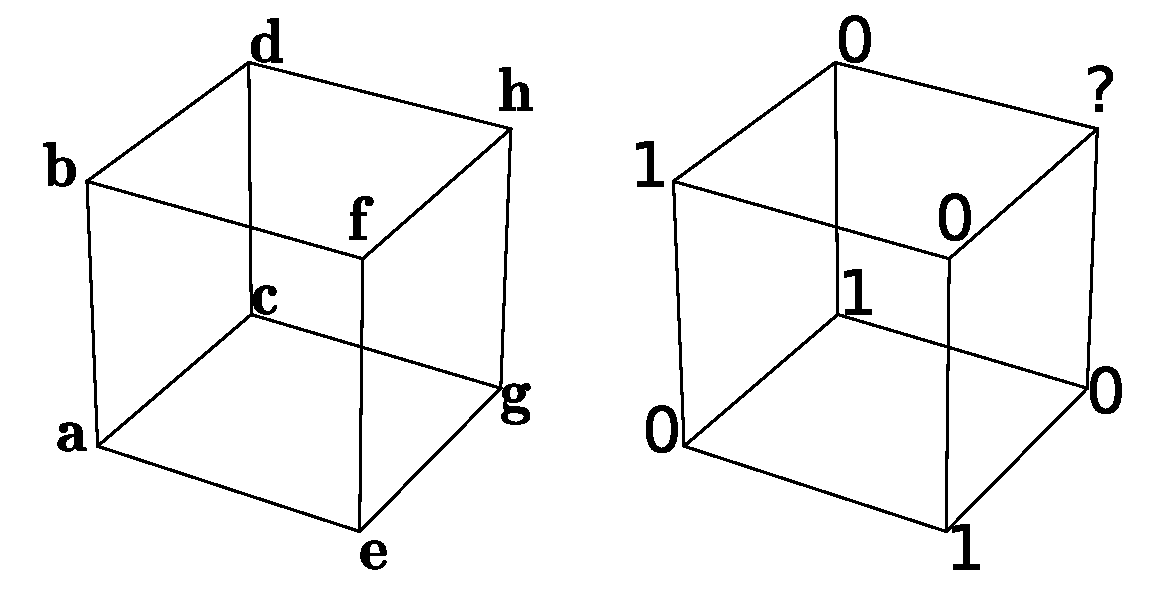
\includegraphics[width=3in]{figures/classification_problem.pdf}
  \caption{A classification problem in $\mathbb{B}^3$. Labels $f(\mathbf{x})$
  are on the right cube.}
\label{FIG:classification_problem}
\end{figure}
We know the values of $f(\mathbf{x})$ for
every single element $\mathbf{x}$ but $\mathbf{h}$, so $S = \{ \mathbf{a}, \mathbf{b},
\mathbf{c}, \mathbf{d}, \mathbf{e}, \mathbf{f}, \mathbf{g}\}$. To guess the
value of $f(\mathbf{h})$, we will use the so-called \textbf{analogical
inference principle}, which states that if four elements $\mathbf{a},
\mathbf{b}, \mathbf{c}, \mathbf{d}$ are in proportion, then their class should
also be in proportion:
$$
\infer{f(\mathbf{a}) : f(\mathbf{b}) :: f(\mathbf{c})
: f(\mathbf{d})}{\mathbf{a} : \mathbf{b} :: \mathbf{c} : \mathbf{d}}
$$

This is obviously an unsound principle, in that the conclusion does not
logically follows from the premise. But as we will see in this document, it can
still be useful.

As we want to guess the value of $f(\mathbf{h})$, this principle leads us to
look for all 3-tuples $(\mathbf{x}, \mathbf{y}, \mathbf{z}) \in S^3$ such that
$\mathbf{x}:\mathbf{y}::\mathbf{z}:\mathbf{h}$.  The analogical inference then
states that we should have
$f(\mathbf{x}):f(\mathbf{y})::f(\mathbf{z}):f(\mathbf{h})$. Figure
\ref{FIG:cubes_in_B3} tells us that there are 6 (non-flat) parallelograms
involving $\mathbf{h}$ as a vertex. The six unique corresponding proportions
are:

\begin{enumerate}
  \item $\mathbf{a} : \mathbf{b} :: \mathbf{g} : \mathbf{h}$
  \item $\mathbf{a} : \mathbf{d} :: \mathbf{e} : \mathbf{h}$
  \item $\mathbf{a} : \mathbf{c} :: \mathbf{f} : \mathbf{h}$
  \item $\mathbf{b} : \mathbf{d} :: \mathbf{f} : \mathbf{h}$
  \item $\mathbf{e} : \mathbf{f} :: \mathbf{g} : \mathbf{h}$
  \item $\mathbf{c} : \mathbf{g} :: \mathbf{d} : \mathbf{h}$
\end{enumerate}

Applying the analogical inference principle to the first proportion $\mathbf{a}
: \mathbf{b} :: \mathbf{g} : \mathbf{h}$ leads to $f(\mathbf{a}) :
f(\mathbf{b}) :: f(\mathbf{g}) : f(\mathbf{h})$, which is equivalent to:
$$0:1::0:f(\mathbf{h}).$$ By referring to Table \ref{TAB:six_valid_patterns}, we
notice that $f(\mathbf{h})$ should be equal to $1$ for the proportion
$f(\mathbf{a}) : f(\mathbf{b}) :: f(\mathbf{g}) : f(\mathbf{h})$ to be a valid
one, because $0:1::0:1$. So we keep $1$ in the back of our head as a possible
candidate for $f(\mathbf{h})$: we say that $1$ is a \textbf{candidate
solution} for $f(\mathbf{h})$.

What we have just done is the \textbf{solving of an analogical equation}.
Generally speaking, an analogical equation is a proportion $a:b::c:x$ in a
context where $x$ is unknown. Determining the value of $x$ is then called the
\textit{solving} of this equation. Depending on the nature and values of $a, b$,
and $c$, there may or may not exist a solution, and it might not be unique. In a
Boolean setting, an equation is solvable for 6 patterns of $a, b, c$ (the 6
patterns of Table \ref{TAB:six_valid_patterns}, naturally). As we can see, the
solution is always unique:

\begin{proposition}
  \label{PROPOS:equation_solving}
  Let $a, b, c$ in $\mathbb{B}$. The analogical equation
  $a :b::c:x$
  is solvable if and only if $a = b$ or $a = c$. The solution denoted
  $\emph{sol}(a, b, c)$ is then given by:
  $$
  \begin{cases}
    \emph{sol}(a, b, c) \eqdef c \emph{ if } a = b,\\
    \emph{sol}(a, b, c) \eqdef b \emph{ if } a = c,
  \end{cases}
  $$
  or more generally:
  $$\emph{sol}(a, b, c) \eqdef c - a + b,$$
  because the Boolean proportion is a particular case of the arithmetic
  proportion.
\end{proposition}

Let's get back to the estimation of $f(\mathbf{h})$. Applying the analogical
inference principle to the second proportion $\mathbf{a} : \mathbf{d} ::
\mathbf{e} : \mathbf{h}$ leads $f(\mathbf{a)} : f(\mathbf{d}) :: f(\mathbf{e})
: f(\mathbf{h})$, and to the solving of $0:0::1:f(\mathbf{h})$. Here again, the
solution is $1$, just like the candidate of the first proportion.
The third proportion  $\mathbf{a} : \mathbf{c} :: \mathbf{f} : \mathbf{h}$
leads to the solving of $0:1::0:f(\mathbf{h})$, also claiming that $1$ is a good candidate.

And now the fourth proportion $\mathbf{b} : \mathbf{d} :: \mathbf{f} :
\mathbf{h}$, which leads to $1:0::0:f(\mathbf{h})$. \textbf{This equation is not
solvable}: neither $1:0::0:1$ nor $1:0::0:0$ are valid proportions. We thus
simply discard the proportion $\mathbf{b} : \mathbf{d} :: \mathbf{f} :
\mathbf{h}$ as a potential source of information about $f(\mathbf{h)}$, because
we are not in a position to apply the analogical inference principle. We can
easily verify that the fifth and sixth (and last!) proportions also lead to
non-solvable equations.

All in all, we are left with three candidates coming from the first three
proportions, all of which are equal to $1$. Our guess will thus be that
$f(\mathbf{h})$ should be equal to $1$. Is this correct? Well in real-world
settings, there is no way to know for sure, because the ground truth function
$f$ is unknown (otherwise, there is no point in trying to classify $\mathbf{h}$
in the first place). The undeniable perks of artificial examples is that we can
do how we please, and define the function $f$ by
$$\forall \mathbf{x}, ~ f(\mathbf{x}) = f(x_1, x_2, x_3) = x_1 \oplus x_2 \oplus x_3,$$
where $\oplus$ denotes the XOR operator, which is both commutative and
associative: $a \oplus b = (a \wedge \neg b) \vee (\neg a \wedge b)$. So in our
case, yes, the true value of $f(\mathbf{h})$ is indeed $1$ and our prediction
is correct.

Notice that we have so far lightheartedly ignored  all the flat proportions.
This is because none of these proportions allow us to derive a solvable
equation. Considering for example $\mathbf{d} : \mathbf{h} :: \mathbf{d} :
\mathbf{h}$, we're led to the solving of $f(\mathbf{d}) : f(\mathbf{h}) ::
f(\mathbf{d}) : f(\mathbf{h})$, or equivalently of $0 : f(\mathbf{h}) :: 0 :
f(\mathbf{h})$. Both values $0$ and $1$ could lead to equally valid proportions
here, so there is simply no predictive power in the flat proportions. We have
also only considered unique proportions, up to equivalence. The first proportion
$\mathbf{a} : \mathbf{b} :: \mathbf{g} : \mathbf{h}$ for example is equivalent
to $\mathbf{a} : \mathbf{g} :: \mathbf{b} : \mathbf{h}$ (using central
permutation), which we could have
used instead. As any two equivalent proportions lead to the same solution for
their associated class equations, we usually choose to ignore all other equivalent
proportions, which allows to divide the number of equation solving by a factor
of $2$.

Here is a small outline of our classification process, that was entirely
governed by the analogical inference principle. Our goal was to guess the value
of $f(\mathbf{h})$:

\begin{itemize}
  \item We first looked at all the $(\mathbf{x}, \mathbf{y}, \mathbf{z}) \in
    \mathbf{B}^3$ such that:
    \begin{itemize}
      \item $f(\mathbf{x}), f(\mathbf{y})$ and $f(\mathbf{z})$ are known ;
      \item $\mathbf{x}:\mathbf{y}::\mathbf{z}:\mathbf{h}$ holds ;
      \item the \textbf{class equation} $f(\mathbf{x}) :f(\mathbf{y}) ::
        f(\mathbf{z}) :s$ is \textbf{solvable}. $s$ is called a
        \textbf{candidate solution}.
    \end{itemize}
    Each of our three candidate solutions $s_1, s_2, s_3$ agreed on the same prediction:
    $s_i = 1$ for all $i$.
  \item We thus estimated that $f(\mathbf{h})$ should indeed be equal to $1$.
\end{itemize}

This minimal example of analogical classification raises a few concerns, which
we will be thoroughly addressed in this document:
\begin{enumerate}
  \item All of the three candidate solutions for $f(\mathbf{h})$ agreed on the
    same prediction: $1$. What if one of them predicted $0$? A first drastic
    option is to refuse to classify $\mathbf{h}$, on the basis that if the
    candidates cannot agree on their predictions, then we should not trust any
    of them. As it will become clear, in practice the candidates never really
    completely agree, even though sometimes a clear majority emerges. So this
    strategy would make the prediction impossible for most elements $\mathbf{x}
    \notin S$. A wiser option is to consider an aggregation of the candidate
    solutions: the most common one, for example. This is the option that has
    been took on so far, as we will see in the next chapter.
  \item Here, by chance, the set of candidate solutions for $f(\mathbf{h})$ was
    not empty: we found three candidate solutions. What happens if we can't
    find any candidate? This case arises when there are no 3-tuple
    $(\mathbf{x}, \mathbf{y}, \mathbf{z}) \in S^3$ such that $\mathbf{x} :
    \mathbf{y}::\mathbf{z}:\mathbf{h}$ and such that the associated equation
    $f(\mathbf{x}):f(\mathbf{y})::f(\mathbf{z}):f(\mathbf{h})$ is solvable. In
    the works of Stroppa and Yvon (\cite{StrYvoCNLL05}), such an $\mathbf{h}$
    cannot be classified. The notion of \textbf{analogical dissimilarity}
    as used in \cite{BayMicDelIJCAI07} will allow to bypass this issue. One of
    the contribution of our work is to provide a unifying view of the two
    techniques, and is the purpose of Chapter \ref{CHAP:functional_definition}.

  \item How \textit{safe} is the analogical inference principle? What are some
    theoretical guarantees that could allow us to use it on a sound basis? This
    question stays, to this day, unanswered. In Chapter \ref{TODO} however, we
    will provide a complete characterization of the Boolean functions $f$ that
    allow to derive sound conclusions.
\end{enumerate}

\paragraph{How many proportions can we build in $\mathbb{B}^m$?\\}
\label{SEC:number_of_parallelograms_in_Bm}

Exactly $6^m$! And it is fairly easy to derive: there are $6$ proportions in
$\mathbb{B}$. As a proportion in $\mathbb{B}^2$ is the concatenation of any two
proportions in $\mathbb{B}$, there are exactly $6^2 = 36$ proportions in
$\mathbb{B}^2$, as seen in Section
\ref{SEC:shortcut_from_aristotle_to_boolean_proportions}. Analogical
proportions in $\mathbb{B}^m$ are defined component-wise, i.e. they are the
concatenation of $m$ proportions in $\mathbb{B}$. Equivalently, a proportion in
$\mathbb{B}^m$ is the concatenation of a proportion in $\mathbb{B}^{m - 1}$ and
a proportion in $\mathbb{B}$. By trivial induction, we can build $6^m$
proportions in $\mathbb{B}^m$.

But let's now ask a more relevant and challenging question: how many
\textit{useful} proportions can we build in $\mathbb{B}^m$? By \textit{useful},
we mean proportions that could be used for classification purposes.

\begin{aquote}{The astute reader, who has been struck by divine light}
  What a silly question! There are obviously $\frac{6^m}{8} - 4^{m - 1} + 2^{m
  - 3}$ such proportions! How can you not be aware of the A016283 sequence from
  the OEIS\footnote{The On-line Encyclopedia of Integer Sequences
  (http://oeis.org/A016283)}?!
\end{aquote}

Unfortunately, we, who have not (yet) been struck by divine light, will have to
derive this formula ourselves. We have seen in Section \ref{TODO} that the only
proportions $\mathbf{a} : \mathbf{b} :: \mathbf{c} : \mathbf{d}$ that are
useful for classification purposes are those where all elements $\mathbf{a},
\mathbf{b}, \mathbf{c}, \mathbf{d}$ are distinct. We thus want to exclude from
the $6^m$ proportions those that comply with one of the following patterns:

\begin{itemize}
  \item $\mathbf{a}: \mathbf{a} :: \mathbf{a} : \mathbf{a}$
  \item $\mathbf{a}: \mathbf{b} :: \mathbf{a} : \mathbf{b}$, and its three
    equivalent forms $\mathbf{a}: \mathbf{a} :: \mathbf{b} : \mathbf{b}$,
    $\mathbf{b}: \mathbf{a} :: \mathbf{b} : \mathbf{a}$, and $\mathbf{b}:
    \mathbf{b} :: \mathbf{a} : \mathbf{a}$
\end{itemize}

Now, let's count them.

\begin{itemize}
  \item Each of the $2^m$ vertex $\mathbf{a}$ will generate a proportion of the
    form $\mathbf{a}: \mathbf{a} :: \mathbf{a} : \mathbf{a}$, so there are
    exactly $2^m$ proportions of this kind.
  \item Every pair $(\mathbf{a}, \mathbf{b})$ of vertices will generate four
    proportions:
    \begin{itemize}
      \item $\mathbf{a}: \mathbf{b} :: \mathbf{a} : \mathbf{b}$,
      \item $\mathbf{a}: \mathbf{a} :: \mathbf{b} : \mathbf{b}$,
      \item $\mathbf{b}: \mathbf{a} :: \mathbf{b} : \mathbf{a}$,
      \item $\mathbf{b}: \mathbf{b} :: \mathbf{a} : \mathbf{a}$.
    \end{itemize}
    There are $\binom{2^m}{2}$ distinct pairs of vertices, so in total this
    makes $4\cdot \binom{2^m}{2}$ proportions of the form $\mathbf{a}: \mathbf{b} ::
    \mathbf{a} : \mathbf{b}$ with its equivalent forms.
\end{itemize}

We are then left with the number of $6^m - 2^m - 4\cdot\binom{2^m}{2}$ useful
proportions. We know that for each of these proportions, all elements
$\mathbf{a}, \mathbf{b}, \mathbf{c}, \mathbf{d}$  are distinct. For each of
them, there are thus 7 other equivalent forms, which reduces the number of
useful and unique (up to equivalence) proportions to:
$$P_m = \frac{1}{8} \left[6^m - 2^m - 4\cdot\binom{2^m}{2} \right].$$
This is precisely the number of non-flat parallelograms in an $m$-dimensional
cube. The A016283 sequence of the OEIS mentioned above actually describes
\textit{the number of rectangles that can be formed from the vertices of an
$m$-dimensional cube}, which is exactly equivalent. Using
the fact that $\binom{n}{k} = \frac{n}{k}\binom{n - 1}{k - 1}$, it can be shown
that the two formulas $\frac{1}{8} \left[6^m - 2^m - 4\cdot\binom{2^m}{2} \right]$
and $\frac{6^m}{8} - 4^{m - 1} + 2^{m- 3}$ are, fortunately, the same.

To be fair, we have no idea how the formula of the OEIS was derived, but we
firmly believe that ours is the most entertaining one. Table
\ref{TAB:n_params_in_cube} gives the values of $P_m$ for the first $10$ values
of $m$.
\begin{table}[h!]
\centering
  \begin{tabular}{ l  l }
\toprule
 $m$ & $P_m$\\
\midrule
    1	&	0\\
    2 &	1\\
    3	&	12\\
    4	&	100\\
    5 &	720\\
    6 &	4816\\
    7 &	30912\\
    8 &	193600\\
    9 & 1194240\\
    10 & 7296256\\
\bottomrule
\end{tabular}
\caption{Number of unique non-flat proportions in an $m$-dimensional cube.}
\label{TAB:n_params_in_cube}
\end{table}
Naturally, $P_2$ and $P_3$ are in accordance with our empirical  results from
Figures \ref{FIG:proportions_in_B2} and \ref{FIG:cubes_in_B3}. The fact that
$P_1 = 0$ means that no inference can be done with analogical proportion in
$\mathbb{B}$, which is perfectly normal: in $\mathbb{B}$, all proportions are
flat (i.e. the pattern is always $a:b::a:b$ or $a:a::b:b$).

\section{Formal definitions}
\label{SEC:formal_definitions_proportions}

The Boolean proportion was introduced in the previous section in an informal
way, along with many key concepts such as the solving on an analogical
equation, and the analogical inference principle. In this section, we will
provide the definition of the Boolean proportion (and others) in a more formal
way.

Probably the first use of formal proportions is that of Lepage in
\cite{Lep04} who, starting from the three aforementioned axioms, formally
defined analogical proportions over alphabets of letters with the aim of
generating (analogical) formal languages. His definition have later been
generalized in the works of Stroppa and Yvon (see \cite{StrYvoCNLL05} and
\cite{StrYvoREPORT05})\footnote{In the same work, Stroppa and Yvon also laid
the foundations of analogical learning as used in this thesis (see Section
\ref{la section})}, who provided an algebraic factorization-based definition of
analogical proportions in semigroups:

\begin{definition}
\label{DEF:proportion_semi_group}
Let $(U, \oplus)$ be a semigroup, i.e. $U$ is a set and $\oplus$ is an
  associative binary operation. Four elements $a, b, c, d \in U$, are in proportion if
  there exist some factorization
  \begin{align*}
    a &= a_1 \oplus a_2 \oplus \cdots \oplus a_n\\
    b &= b_1 \oplus b_2 \oplus \cdots \oplus b_n\\
    c &= c_1 \oplus c_2 \oplus \cdots \oplus c_n\\
    d &= d_1 \oplus d_2 \oplus \cdots \oplus d_n,
  \end{align*}

  such that for all $i \in [1, n]$, 
  $$
  \begin{cases}
    a_i = b_i \emph{ and } c_i = d_i\\
    \emph{or}\\
    a_i = c_i \emph{ and } b_i = d_i.
  \end{cases}
  $$
\end{definition}

We can clearly foresee here the features of the Boolean proportion. It will be
insightful to instantiate $U$ as the set of natural number $\mathbb{N}$ and
$\oplus$ as the usual multiplication $\times$. In this setting, let's consider
the prime factorization of:

\begin{align*}
  a &= 30 = 1 \times 2 \times 3 \times 5\\
  b &= 60 = 2 \times 2 \times 3 \times 5\\
  c &= 25 = 1 \times 1 \times 5 \times 5\\
  d &= 50 = 2 \times 1 \times 5 \times 5
\end{align*}

For each $i$, we either have $a_i = b_i$ and $c_i = d_i$ ($i = 2, 3, 4$) or
$a_i = c_i$ and $b_i = d_i$ ($i = 1, 4$). We can then say that $a, b, c, d$ are
in proportion, i.e. $30: 60 :: 25:50$. Naturally, the reader will recognize
here the geometric proportion: $\frac{30}{60} = \frac{25}{50}$.
Starting from this general definition, other proportions have been defined in
various domains, namely analogies between trees, lattices, or matrices
\cite{MicDel04, StrYvoREPORT05, MicBayDelJAIR08}. However, we will not detail
them further here and rather focus on other domains of interest.

In \cite{Lep03}, Lepage defines an analogy between sets as follows: four subsets
$A, B, C, D$ of a universal set $X$ are in proportion if $A$ can be transformed
into $B$ by adding and deleting the same elements as to transform $C$ into $D$.
A more formal definition has been given in \cite{StrYvoREPORT05}:

\begin{definition}
  \label{DEF:analogy_set_facto}
  Let $A, B, C, D \subset X$. $A, B, C, D$ are in proportion if there exists
  four subsets $U, V, W$ and $Z$ (not necessarily disjoint) such that:
  $$
  \begin{cases}
    A = U \cup V\\
    B = U \cup W\\
    C = Z \cup V\\
    D = Z \cup W\\
  \end{cases}
  $$
\end{definition}

To go from $A$ to $B$, one needs to add $W$ and remove $V$. To go from $C$ to
$D$, one needs to do the exact same thing: add $W$ and remove $V$. An
equivalent definition has been given in \cite{MicPra09}:

\begin{definition}
  \label{DEF:analogy_set_miclet_henri}
  Let $A, B, C, D \subset X$. $A, B, C, D$ are in proportion if:
  $$
  A \setminus B = C \setminus D \emph{ and } B \setminus A = D \setminus A
  $$
\end{definition}

Definition \ref{DEF:analogy_set_miclet_henri} reads as \textit{$A$ differs from
$B$ as $C$ differs from $D$, and $B$ differs from $A$ as $D$ differs from $C$},
which is naturally equivalent to the statement of Definition
\ref{DEF:analogy_set_facto}: $A \setminus B = C \setminus D = V$, and $B
\setminus A = D \setminus A  = W$. The formula of Definition
\ref{DEF:analogy_set_miclet_henri} is actually equivalent to the following form
(not without using various ingenious tweaks): $$A \cup D = B \cup C \text{ and
} A \cap D = B \cap C.$$

As an example, let's consider $A = \{a, b, c, g\}, B = \{a, b, d, e, g\}, C =
\{c, f, g\}$ and $D = \{d, e, f, g\}$, as summed-up in Table
\ref{TAB:analogy_sets}.

\begin{table}[h!]
\centering
$$
\begin{tabular}{ c  c  c  c  c  c  c  c }
\toprule
  & a & b & c & d & e & f & g\\
\midrule
  A & \times & \times & \times &  &  &  & \times \\
  B & \times & \times &  & \times & \times &  & \times\\
  C &  &  & \times &  &  & \times & \times\\
  D &  &  &  & \times & \times & \times & \times\\
\bottomrule
\end{tabular}
$$
\caption{Four sets $A, B, C, D$ in analogical proportion.}
\label{TAB:analogy_sets}
\end{table}

Setting $U = \{a, b, g\}, V = \{c\}, W = \{d, e\}$ and $Z = \{f, g\}$, the
conditions of Definition  \ref{DEF:analogy_set_facto}  are clearly satisfied.
Also, $A \setminus B = C \setminus D = \{c\} = V$, and $B\setminus A = D
\setminus C = \{d, e\} = W$. Finally, $A \cup D = B \cup C = \{a, b, c, d, e,
f, g\}$ and $A\cap D = B\cap C = \{g\}$.

We can also recognize in Table \ref{TAB:analogy_sets} that the conditions of
Definition \ref{DEF:proportion_semi_group} are satisfied, i.e. for all $i$ we
have either $A_i = B_i$ and $C_i = D_i$, or $A_i = C_i$ and $B_i = D_i$.

The definition of the Boolean proportion can be directly derived from
Definition \ref{DEF:analogy_set_miclet_henri} and by considering the set
$\mathbb{B} = \{0, 1\}$:

\begin{definition}
  \label{DEF:boolean_proportion}
  Four elements $a, b, c, d$ in $\mathbb{B} = \{0, 1\}$ are in proportion if
  \begin{alignat*}{2}
    &(a \leftrightarrow b \wedge c \leftrightarrow d) && \vee (a
    \leftrightarrow c \wedge b \leftrightarrow d), \emph{ or equivalently}\\
     & (a \wedge d \leftrightarrow b \wedge c) &&\wedge (a \vee  d
    \leftrightarrow b \vee c),
  \end{alignat*}
  where $\leftrightarrow$ stands for the equivalence connective.
\end{definition}

These scary formulas state the exact same facts as the previous definition,
i.e. that $a$ differs from $b$ as $c$ differs from $d$ and conversely $b$
differs from $a$ as $d$ differs from $c$. Naturally, Definition
\ref{DEF:boolean_proportion} and \ref{DEF:boolean_proportion_informal} (the one
we initially suggested) are equivalent.

We now have to go back to the 80's and mention the pioneering work of Sheldon
Klein, who, to some extent, defined his \textit{own} Boolean analogical
proportion. His definition states that $a, b, c, d$ in $\mathbb{B}$ are in
proportion if $a \oplus b = c \oplus d$, where $\oplus$ is the XOR operator.
This definition, less restrictive than Definition \ref{DEF:boolean_proportion},
amounts to adding two new patterns to Table \ref{TAB:six_valid_patterns}:
$0:1::1:0$, and its counterpart $1:0::0:1$. These two patterns seem appealing at
first sight, because they capture the fact that $a : \neg a :: b \neg b$.
However, they lead to the fact that $a:b::c:d$ if and only if $b : a :: c :d$,
which seems quite unnatural for an analogy. In Section \ref{TODO}, we will show
that the two definitions of Boolean proportion (the standard one of Definition
\ref{DEF:boolean_proportion} and that of Klein) share common properties with
regard to their suitability with the analogical inference principle. We will
also see that in spite of this, the standard model seems to be the most useful
one in practice.

The notion of Boolean analogical proportion has recently been extended to the
concept of \textbf{logical proportion} (see e.g. \cite{PraRic14}), but their
details are out of the scope of this document.


\chapter{A functional definition of analogical classifiers}
\label{CHAP:functional_definition}
\localtableofcontents*
\vspace*{\baselineskip}

\initial{I}n Section \ref{SEC:machine_learning_with_boolean_proportions}, we
briefly described a basic process of analogical classification in an informal
way, making sure that everything went smoothly. In practice, bad things happen,
always. In this chapter, we will clearly and formally define analogical
classification, which will help us clarify some of the grey areas of Section
\ref{SEC:machine_learning_with_boolean_proportions}. Also (and most
importantly), we will describe our contributions to this problem.

A first form of analogical classifiers has been defined in the works of Stroppa
and Yvon \cite{StrYvoCNLL05}, which we will refer to as \textbf{conservative
classifiers}. Another form of analogical classifiers has later been proposed in
the works of Bayoudh, Delhay and Miclet \cite{MicBayDelJAIR08,
BayMicDelIJCAI07}, referred-to here as \textbf{extended classifiers}.

Though the theoretical groundings of the conservative and extended
classifiers have a lot in common (they are both analogical classifiers after
all), we will see that their practical implementation are actually quite
different. We will show however that the extended classifier is a
generalization of the conservative one, and most importantly that these two
approaches can be factorized into a single, unifying framework.

So far, only algorithmic descriptions of both methods were available. Our
unifying framework will allow us to give a general and \textbf{functional}
definition of analogical classifiers, opening the door to some theoretically
grounded research.

This chapter is structured as follows. In Section
\ref{SEC:analogical_classification}, we will review and detail the two previous
approaches to analogical classification, that we will name here the
conservative and the extended classifiers. We will se that these two approaches
can be factorized into a single functional description. Thanks to this
functional definition of analogical learners, we will be able in Section
\ref{SEC:theoretical_properties_of_analogical_classifiers} to derive some
theoretical properties about analogical learners. We will indeed show that
their VC-dimension is infinite, and that their accuracy is closely related to
that of the $k$-NN classifier. Finally in Section
\ref{SEC:experiments_and_empirical_validation}, we will empirically verify our
results and provide some insights that will motivate the topic of Chapter
\ref{CHAP:analogy_preserving_functions}.

\section{Analogical classification}
\label{SEC:analogical_classification}

This first section will be devoted to the unification of two seemingly
different analogical approaches to classification.  Let us first define the
problem of classification, one of the main subfields of machine learning. The
aim is simple: a classifier has to estimate the class of any element given as
input on the basis of some other elements for which the class is known.
Formally, we denote $X^m$ our universe which is usually a Cartesian product:
$X^m = X_1 \times X_2 \times \ldots \times X_m$. We have at our disposal a
subset $S \subsetneq X^m \times Y$ of $n$ pairs $\left(\mathbf{x},
f(\mathbf{x})\right)$, called the \textbf{training set}.  $$S=
\Set{\left(\mathbf{x}^{(i)}, f(\mathbf{x}^{(i)})\right) \in X^m \times Y | i
\in [1,n]}.$$

For any $\mathbf{x} \in X^m$, the value $f(\mathbf{x})$ is called its
\textbf{class} or \textbf{label}.
The functional notation $f(\mathbf{x})$ suggests that all labels
are defined by an underlying function $f \colon X^m \to Y$, which is the usual
general view point of machine learning. In the case of classification, $Y$ is a
finite set of size $C$ where $C$ is the number of different classes. The goal
of a classifier is to \textbf{learn} the function $f$ on the basis of the
elements in $S$, called the \textbf{examples}. The output of a classifier is a
function $\hat{f} \colon X^m \to Y$ that is \textit{as close as possible} the
ground truth function $f$.

\subsection{Conservative classifier}
\label{SEC:conservative_classifier}

We will here describe what we call a \textbf{conservative} classifier. Without
further ado, let us consider Algorithm \ref{ALGO:conservative_classifier} which
describes such classifiers.

\begin{algorithm}[!ht]
\caption{The Conservative classifier.}
\label{ALGO:conservative_classifier}
  \begin{algorithmic}
    \STATE {\bf Input}: A training set $S$ and an element $\mathbf{x} \in X^m
    \setminus S$ for which $f(\mathbf{x})$ is unknown.
    \STATE {\bf Output}: $\hat{f}(\mathbf{x})$, an estimation of
    $f(\mathbf{x})$.
    \STATE {\bf Init}: $\mathbf{C}(\mathbf{x}) = \varnothing$ \quad \quad // A multiset of candidate
    labels.

    \FORALL{$(\mathbf{a}, \mathbf{b}, \mathbf{c}) \in S^3$ such that
    $\mathbf{a} : \mathbf{b} :: \mathbf{c} : \mathbf{x}$}
    \IF{$f(\mathbf{a}) : f(\mathbf{b}) ::f(\mathbf{c}) : y$ is
    solvable}
    \STATE $y = \sol\left(f(\mathbf{a}), f(\mathbf{b}), f(\mathbf{c})\right)$
    \STATE $ \mathbf{C}(\mathbf{x}) = \mathbf{C}(\mathbf{x}) \cup y$
    \ENDIF
	  \ENDFOR
    \STATE $\hat{f}(\mathbf{x}) = \text{Mode} (\mathbf{C}(\mathbf{x}))$ // The most common value in
    $\mathbf{C}(\mathbf{x})$ (undefined if $\mathbf{C}(\mathbf{x}) = \varnothing$).
  \end{algorithmic}
\end{algorithm}

It should be easy to see that the process of Algorithm
\ref{ALGO:conservative_classifier} is extremely similar to the one we followed
on our first introduction to classification with Boolean proportions in
Section \ref{SEC:machine_learning_with_boolean_proportions}. Here again the key
underlying process is the analogical inference principle, which states that if
four elements are in proportion, then their classes should also be in
proportion. But Algorithm \ref{ALGO:conservative_classifier} is slightly more
general than what we have glimpsed in Section
\ref{SEC:machine_learning_with_boolean_proportions}: it allows to deal with
cases where some of the candidate solutions $y$ do not agree with each other.
The fix here is to consider that the prediction $\hat{f}(\mathbf{x})$ will be
the most common candidate solution among all the predictors. This definition of
analogical classification comes from the work of Stroppa and Yvon
\cite{StrYvoCNLL05, StrYvoREPORT05}, and to our knowledge it is the first
instance of analogical learner that has ever been proposed. We note however
that the authors did not explicitly state that the class equations must be
solvable to be useful.

Note that if the multiset $\mathbf{C}(\mathbf{x})$ is empty, i.e. if we cannot find
$3$-tuples in $S^3$ such that they are in proportion with $\mathbf{x}$ and such
that the related class equation is solvable, then the value
$\hat{f}(\mathbf{x})$  is undefined and $\mathbf{x}$ cannot be classified
(hence the name \textit{conservative}).

At first sight, we are here in a setting where the examples in $S$ are stored
for future use, without any generalization process.  We will thus consider (for
now) that the conservative classifier ranges among the category of
\textbf{lazy learners}, i.e. learners that only rely on the training set $S$
without any actual \textit{learning} stage, or without building any model of
the data. The most popular instance of lazy learner certainly is the famous
$k$-NN algorithm.

In the following, we will give a functional definition of $\hat{f}(\mathbf{x})$
as outputted by a conservative classifier. To this end, we will define two
crucial concepts: the \textbf{analogical extension} of a training set $S$, and
the \textbf{analogical root} of an element $\mathbf{x}$. Both the analogical
extension and the analogical root were first defined in \cite{StrYvoREPORT05},
with some minor differences with our definitions.

\begin{definition}[Analogical extension]
  \label{DEF:analogical_extension}
  Denoting $S$ a training set and $f$ the ground truth function of the labels,
  the \textbf{analogical extension} of $S$ using $f$ is:
  $$
  \esf \eqdef \Set{ \mathbf{x} \in X^m |  \exists
  (\mathbf{a},\mathbf{b},\mathbf{c}) \in S^3, ~ \mathbf{a} : \mathbf{b} ::
  \mathbf{c} : \mathbf{x} \text{ and } f(\mathbf{a}) : f(\mathbf{b}) ::
  f(\mathbf{c}) : y \text{ is solvable}}.
  $$
\end{definition}

Intuitively,  $\esf$ can be regarded as the set of all $\mathbf{x} \in X^m$
that are in proportion with at least one 3-tuple in $S$, provided that the
equation related to the associated labels is also solvable. For any $S$ and any
$f$, $\esf$ satisfies some interesting properties: \begin{enumerate}
\item $S \subseteq \esf$, since $\mathbf{x} : \mathbf{x} :: \mathbf{x}
  :\mathbf{x}$ always holds;
\item $\aext{\varnothing}{f} = \varnothing$, and $\aext{X^m}{f}=X^m$;
\item $S_1 \subseteq S_2 \implies \aext{S_1}{f} \subseteq \aext{S_2}{f}$.
\end{enumerate}
We will denote by $\esfs$ the set of elements in $\esf$ that are not in $S$:
$$\esfs \eqdef \esf \setminus S.$$ In a setting where for any
$\mathbf{a},\mathbf{b}, \mathbf{c}$ the equation $\mathbf{a} : \mathbf{b} ::
\mathbf{c} : \mathbf{x}$ is always solvable (as is the case for the arithmetic
proportion) and such that the associated class equation is also solvable, we
can show that the size of $\esfs$ is exactly $\frac{1}{2} n^2(n - 1)$. This
value is thus a loose upper bound for $\mid \esfs\mid$, because in practice
equations are not always solvable.

\begin{testexample}
To polish our understanding of the analogical extension, let us consider Figure
\ref{FIG:ae_example}.
The training set $S$ is $\Set{\mathbf{a}, \mathbf{b}, \mathbf{d},\mathbf{e}}$.
Taking $(\mathbf{b}, \mathbf{d}, \mathbf{a}) \in S^3$, we notice that
$\mathbf{b} : \mathbf{d} :: \mathbf{a} : \mathbf{c}$, and the associated class
equation $0:1::0:y$ is solvable. So $\mathbf{c}$ is in $\esf$. The same goes for
$\mathbf{f}$ with the 3-tuple $(\mathbf{a}, \mathbf{b}, \mathbf{e}) \in S^3$.
However, even if we can find $(\mathbf{b}, \mathbf{d}, \mathbf{e}) \in S^3$
such that $\mathbf{b} : \mathbf{d} :: \mathbf{e} : \mathbf{g}$, the associated
class equation $0:1::1:y$ is not solvable, so $\mathbf{g} \notin \esf$. At
last, vertex $\mathbf{h}$ will suffer the same fate because the class equation
$f(\mathbf{a}) : f(\mathbf{e}) :: f(\mathbf{d}) : y$ is not solvable either. In
the end, $\esf = \set{\mathbf{a}, \mathbf{b}, \mathbf{c}, \mathbf{d},
\mathbf{e}, \mathbf{f}}$ and $\esfs = \Set{\mathbf{c}, \mathbf{f}}$.
\end{testexample}

\begin{figure}[!h]
\centering
  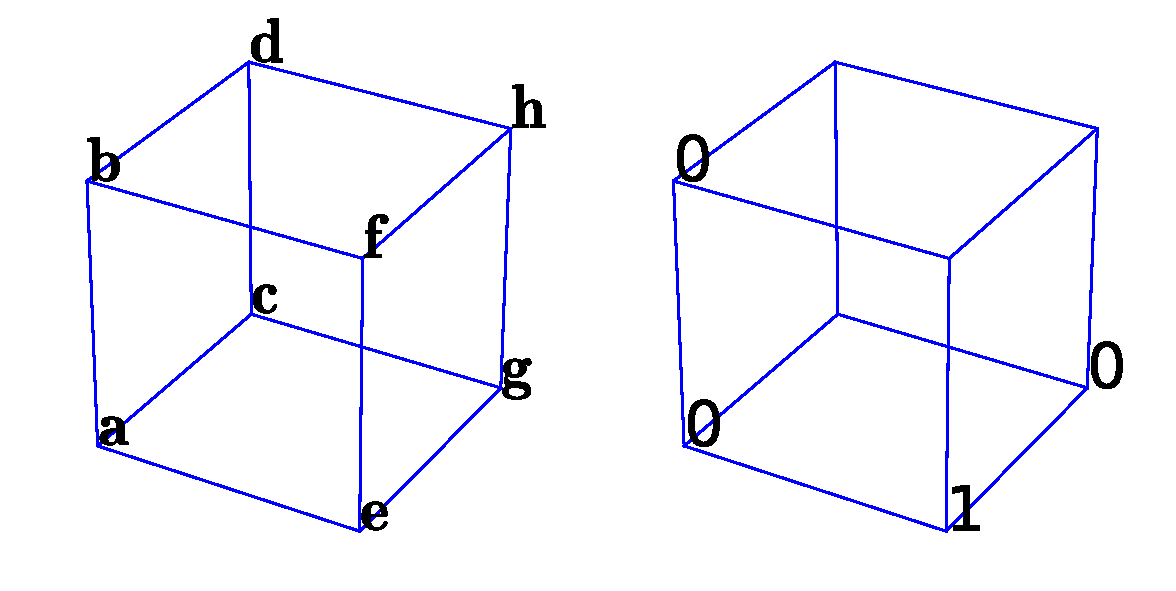
\includegraphics[width=3in]{figures/ae_example.pdf}
  \caption{With $S = \Set{\mathbf{a}, \mathbf{b}, \mathbf{d},
  \mathbf{e}}$, we have $\esfs = \Set{\mathbf{c}, \mathbf{f}}$.}
\label{FIG:ae_example}
\end{figure}

The dual concept of the analogical extension is what we call the
\textbf{analogical root} of a given element $\mathbf{x} \in X^m$:

\begin{definition}[Analogical root]
  \label{DEF:analogical_root}
  Denoting $S$ a training set and $f$ the ground truth function of the labels,
  the \textbf{analogical root} of an element $\mathbf{x} \in X^m$ is:
  $$
  \rsfx \eqdef \Set{(\mathbf{a}, \mathbf{b}, \mathbf{c}) \in S^3 |
  \mathbf{a}:\mathbf{b}::\mathbf{c}:\mathbf{x} \text{ and }
  f(\mathbf{a}):f(\mathbf{b})::f(\mathbf{c}):y \text{ is solvable}}.
  $$
\end{definition}

\noindent
$\rsfx$ is simply the set of 3-tuples in $S$ which are analogically linked to
$\mathbf{x}$.

\begin{testexample}
Considering again the example of Figure \ref{FIG:ae_example}, we have that
$\aroot{S}{f}{\mathbf{c}} = \Set{(\mathbf{b}, \mathbf{d},\mathbf{a}),
(\mathbf{b}, \mathbf{a},\mathbf{d})}$. However, the two corresponding
proportions $\mathbf{b}: \mathbf{d}::\mathbf{a}:\mathbf{c}$ and $\mathbf{b}:
\mathbf{a}::\mathbf{d}:\mathbf{c}$ are equivalent, and we will follow the
convention that the analogical root should only contain non-equivalent
3-tuples, so technically $\aroot{S}{f}{\mathbf{c}}$ is entirely described by
$\Set{(\mathbf{b}, \mathbf{d},\mathbf{a})}$.  We also have that
$\aroot{S}{f}{\mathbf{f}} = \Set{(\mathbf{a}, \mathbf{b},
\mathbf{e})}$, $\aroot{S}{f}{\mathbf{a}} = \Set{(\mathbf{a}, \mathbf{a},
\mathbf{a}), (\mathbf{b}, \mathbf{b}, \mathbf{a}), (\mathbf{d}, \mathbf{d},
\mathbf{a}), (\mathbf{e}, \mathbf{e}, \mathbf{a})}$, and
$\aroot{S}{f}{\mathbf{h}} = \varnothing$. \end{testexample}

It is clear that in general, $$\rsfx = \varnothing\iff \mathbf{x} \notin
\esf.$$ It should also be clear that even if we only consider unique 3-tuples
(up to equivalence) in the analogical root, $\rsfx$ may contain more than one
3-tuple: for example in $\mathbb{R}^m$ or $\mathbb{B}^m$ with the arithmetic
(or Boolean) proportion, $\mathbf{x}$ may be the involved in more than one
parallelogram, as illustrated in Figure \ref{FIG:multiple_parallelograms}.

\begin{figure}[!h]
\centering
  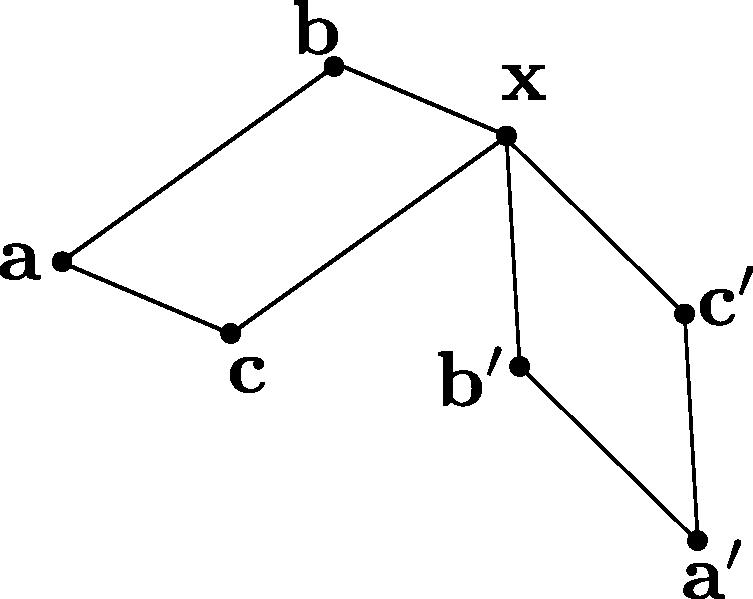
\includegraphics[width=2.5in]{figures/multiple_parallelograms.pdf}
  \caption{With $S = \Set{\mathbf{a}, \mathbf{b}, \mathbf{c}, \mathbf{a}',
  \mathbf{b}', \mathbf{c}'}$, we have $\mathbf{x} \in \esf$ and $\rsfx =
  \Set{(\mathbf{a}, \mathbf{b}, \mathbf{c}), (\mathbf{a}', \mathbf{b}',
  \mathbf{c}')}$. Class equations are all assumed to be solvable.}
\label{FIG:multiple_parallelograms}
\end{figure}

We need to introduce one last definition before we can go on with the
functional view of conservative classifiers:

\begin{definition}[Analogical label]
  \label{DEF:analogical_label}
  For any element $\mathbf{x}$ of $\esf$, we denote $\mathbf{C}(\mathbf{x})$
  the set of the class equations solutions associated with $\mathbf{x}$:
  $$\mathbf{C}(\mathbf{x}) \eqdef \Set{y | f(\mathbf{a}) : f(\mathbf{b}) ::
  f(\mathbf{c}) :y, \quad \text{with }(\mathbf{a}, \mathbf{b}, \mathbf{c}) \in \rsfx}$$
  We then define the \textbf{analogical
  label} of $\mathbf{x}$, denoted $\albl{\mathbf{x}}$, as:
  $$\albl{\mathbf{x}} \eqdef
  \begin{cases}
    f(\mathbf{x}) \text{ if } \mathbf{x} \in S\\
    \text{Mode} \left(\mathbf{C}(\mathbf{x})\right) \text{ if
    } x \notin S
  \end{cases}
  $$
  where $\text{Mode}(\mathbf{C})$ returns the most frequent element of the multiset
$\mathbf{C}$. In case of a tie, the returned element is chosen at random between
the most frequent elements.
\end{definition}

We are now in position to give a functional definition of the conservative
classifier:

\begin{definition}[Conservative classifier]
  \label{DEF:conservative_classifier}
  Given a training set $S$ with an underlying ground truth function $f$,
  a conservative classifier sets the prediction of an element $\mathbf{x}$ as
  follows:

  $$\text{If } \mathbf{x} \in \esf, ~ \hat{f}(\mathbf{x}) \eqdef \albl{\mathbf{x}}.
  \text{ Else, } \hat{f}(\mathbf{x}) \text{ is undefined.}$$
\end{definition}

As previously mentioned, a conservative classifier is not able to output a
prediction if $\mathbf{x}$ does not belong to the analogical extension. We have
already made this observation when describing Algorithm
\ref{ALGO:conservative_classifier}: for a given $\mathbf{x}$, the set of
candidate solutions $\mathbf{C}(\mathbf{x})$ is empty if and only if
$\mathbf{x} \notin \esf$.  Also, we now understand why $\albl{\mathbf{x}}$ is
simply set to $f(\mathbf{x})$ when the $\mathbf{x} \in S$: for such an
$\mathbf{x}$ it is natural to want $\hat{f}(\mathbf{x}) = f(\mathbf{x})$!

\begin{testexample}
Going
back to our example with Figure \ref{FIG:ae_example}, we will have
$\hat{f}(\mathbf{c}) \eqdef \albl{\mathbf{c}} = 1$, because
$\aroot{S}{f}{\mathbf{c}} = \Set{(\mathbf{b}, \mathbf{d},\mathbf{a})}$ and
$\mathbf{C}(\mathbf{c}) = \Set{1}$. Also, $\hat{f}(\mathbf{f}) \eqdef
\albl{\mathbf{f}} = 1$, because $\aroot{S}{f}{\mathbf{f}} =
\Set{(\mathbf{a},\mathbf{b},\mathbf{e})}$ and $\mathbf{C}(\mathbf{f}) =
\Set{1}$. Here, we did not need to use the majority vote procedure as there was
only one candidate solution for each prediction. As $\mathbf{g}$ and
$\mathbf{h}$ do not belong to $\esf$, both $\albl{\mathbf{g}}$ and
$\albl{\mathbf{h}}$ stay undefined.
\end{testexample}

Let us note that in Algorithm \ref{ALGO:conservative_classifier}, the
analogical extension $\esf$ is never explicitly computed. Instead, for a given
$\mathbf{x}$, we look for
every 3-tuple in $S^3$ and check if they belong to $\rsfx$. One drawback is
that the search in $S^3$ has to be done for every new element $\mathbf{x}$ that
we want to classify, and can prove to be quite expensive in computation time,
even for small sizes of $S$. However, taking advantage of our functional
definition, we can reformulate the learning process of a conservative
classifier as follow:

\begin{itemize}
\item First, compute $\esf$. While $\esf$ is begin computed, it is trivial to
  also compute the set of candidates $\mathbf{C}(\mathbf{x})$ for each $x \in
    \esf$.
  \item Then, for all $x \in\esf$, compute
    $\albl{\mathbf{x}} \eqdef \text{Mode}(\mathbf{C}(\mathbf{x}))$.
\end{itemize}
\noindent
Whenever we are asked to classify a given $\mathbf{x}$, all we need now is to
check whether $\mathbf{x}$ belongs to $\esf$ or not. The output
$\hat{f}(\mathbf{x})$ is then immediate. This way to proceed has the undeniable
advantage to perform the search in $S^3$ only once. Obviously, this saving in
computation time is done at the expense of memory consumption, because the
size of $\esf$ can be drastically greater than that of $S$. This alternative
view also leads us to reconsider our previous statement about conservative
classifiers belonging to the class of lazy learners. Here, the computation of
the analogical extension can be viewed as a generalization process, even if not
all elements of the universe $X^m$ are affected by this generalization.

We will end this Section on conservative classifier by sketching a use-case
described in \cite{StrYvoREPORT05}, where an analogical proportion is defined
on the set of words over a finite alphabet, and the task is to learn the
conjugation of English verbs. This setting is slightly different than that of
classification that we have settled-in, but all definitions and concepts remain
valid. Here, solving the analogical equation
$\text{view}:\text{reviewer}::\text{search}:y$ leads to $\text{researcher}$,
using the definition of the analogy and the concatenation operator.
We have a training set $S=\Set{\mathbf{x}^{(1)},\mathbf{x}^{(2)},
\mathbf{x}^{(3)}, \mathbf{x}^{(4)}, \mathbf{x}^{(5)}}$ where
$\mathbf{x}^{(1)}=(read,3,reads), \mathbf{x}^{(2)}=(read,G,reading),
\mathbf{x}^{(3)}=(view,3,views)$, $\mathbf{x}^{(4)}=(view,G,viewing),
\mathbf{x}^{(5)}=(eat,3,eats)$. $(read,3,reads)$ means that $read$ is
transformed into $reads$ when conjugated at the third person singular, and $G$
stands for the gerund form.

Given a new element $\mathbf{x}=(eat,G,y)$, $\rsfx=
\Set{\left(\mathbf{x}^{(1)}, \mathbf{x}^{(2)}, \mathbf{x}^{(5)}\right),
\left(\mathbf{x}^{(3)},\mathbf{x}^{(4)},\mathbf{x}^{(5)}\right)}$. The
prediction is as expected $\hat{f}(\mathbf{x})=\text{eating}$, which is the
solution of the equations $\text{read}:\text{reading}::\text{eat}:y$ and
$\text{view}:\text{viewing}::\text{eat}:y$. There is
no solution for $\mathbf{x}=(absurd,G,y)$, just because $\rsfx= \varnothing$.

The fact that conservative learners cannot output a prediction for any
$\mathbf{x}$ can here be considered a good thing: it would not be natural to
look for the gerund form of \textit{absurd}. However, in many use cases we do
want our classifier to be able to predict the label of any element. This is why
other options have been implemented to overcome this problem, and to extend in
some sense the generalization ability of analogical learners. This is the
purpose of \textbf{extended classifiers} described in the next section.

\subsection{Extended classifier}
\label{SEC:extended_classifier}

We now want our analogical classifier to be able to predict the label of any
input element $\mathbf{x} \in X^m$, and not just the ones in $\esf$.
The main bottleneck of Algorithm \ref{ALGO:conservative_classifier} is that we
require the 3-tuples in $S^3$ to be in perfect proportion with the element
$\mathbf{x}$ we want to classify. Such 3-tuples are not always available in the
training set, so necessarily some elements of $X^m$ are excluded from $\esf$.

The key concept that will help us overcome this issue is what we call an
\textbf{analogical dissimilarity}, first introduced in
\cite{BayMicDelIJCAI07}. The analogical dissimilarity is a measure that
quantifies in some sense \textit{how far} a relation $\mathbf{a} : \mathbf{b}
:: \mathbf{c} : \mathbf{d}$ is from being a perfectly valid proportion.

We keep the initial notation $\AD(\mathbf{a}, \mathbf{b},
\mathbf{c},\mathbf{d})$ to denote the analogical dissimilarity between 4
elements.  Some  minimal properties have to be satisfied by such a
dissimilarity $\AD \colon {(X^m)}^4 \longrightarrow \mathbb{R}^+$ to fit
with the intuition. For any $\mathbf{a}, \mathbf{b},\mathbf{c},\mathbf{d},
\mathbf{e}, \mathbf{f} \in X^m$, the following properties should hold:
\begin{itemize}
  \item $\AD(\mathbf{a}, \mathbf{b},\mathbf{c},\mathbf{d})=0 \iff \mathbf{a} :
    \mathbf{b}:: \mathbf{c} : \mathbf{d}$ (Consistency with the Analogy)
  \item $\AD(\mathbf{a}, \mathbf{b},\mathbf{c},\mathbf{d})=
    \AD(\mathbf{c}, \mathbf{d},\mathbf{a},\mathbf{b})$ (Symmetry)
  \item $\AD(\mathbf{a}, \mathbf{b},\mathbf{c},\mathbf{d})=
    \AD(\mathbf{a}, \mathbf{c},\mathbf{b},\mathbf{d})$ (Central permutation)
  \item $\AD(\mathbf{a}, \mathbf{b},\mathbf{e},\mathbf{f}) \leq \AD(\mathbf{a},
    \mathbf{b},\mathbf{c},\mathbf{d}) + \AD(\mathbf{c},
    \mathbf{d},\mathbf{e},\mathbf{f})$ (Triangle inequality)
  \item In general, $\AD(\mathbf{a}, \mathbf{b},\mathbf{c},\mathbf{d}) \neq
    \AD(\mathbf{b}, \mathbf{a},\mathbf{c},\mathbf{d})$
\end{itemize}
Naturally, the symmetry and central permutation properties lead to the same
three classes of equivalence that we have for the analogical proportion. In
particular, the equivalence class that is \textit{generated} by
$\AD(\mathbf{a}, \mathbf{b},\mathbf{c},\mathbf{d})$ is:
\begin{align*}
  &\AD(\mathbf{a}, \mathbf{b},\mathbf{c},\mathbf{d}) =
\AD(\mathbf{c}, \mathbf{d},\mathbf{a},\mathbf{b})=
\AD(\mathbf{c}, \mathbf{a},\mathbf{d},\mathbf{b})=
\AD(\mathbf{d}, \mathbf{b},\mathbf{c},\mathbf{a})=
\AD(\mathbf{d}, \mathbf{c},\mathbf{b},\mathbf{a})=\\
  &\AD(\mathbf{b}, \mathbf{a},\mathbf{d},\mathbf{c})=
\AD(\mathbf{b}, \mathbf{d},\mathbf{a},\mathbf{c})=
\AD(\mathbf{a}, \mathbf{c},\mathbf{b},\mathbf{d}).
\end{align*}

The definition of an analogical proportion strongly relies on the structure and
operators available on $X^m$, and the same goes for the definition of the
analogical dissimilarity: there are a lot of possibilities. For the arithmetic
proportion in $\mathbb{R}^m$, the analogical dissimilarity  $\AD(\mathbf{a},
\mathbf{b},\mathbf{c},\mathbf{d})$ should capture \textit{how far}
are $\mathbf{a}, \mathbf{b},\mathbf{c},\mathbf{d}$ from making up a perfect
parallelogram. This can be achieved using the following definition:

% Note: leave \emph{AD} here else it will be in italics.
\begin{definition}[Analogical dissimilarity for real vectors]
  \label{DEF:AD_arithmetic_proportion}
  Given four vectors $\mathbf{a}, \mathbf{b},\mathbf{c},\mathbf{d}$ of
  $\mathbb{R}^m$ equipped with the standard $p$-norm $\norm{p}{\cdot}$, the
  analogical dissimilarity related to the arithmetic proportion is defined as:
  $$\text{AD}(\mathbf{a}, \mathbf{b},\mathbf{c},\mathbf{d}) =
  \norm{p}{(\mathbf{a} - \mathbf{b}) - (\mathbf{c} - \mathbf{d})}.$$
\end{definition}

Of course, we will need an analogical dissimilarity in $\mathbb{B}^m$, but we
will start small and consider $\mathbb{B}$ first:
\begin{definition}[Analogical dissimilarity for Boolean vectors]
  \label{DEF:AD_boolean_proportion}
  Given four elements $a, b, c, d$ of $\mathbb{B}$, the analogical
  dissimilarity $\text{AD}(a, b, c, d)$ is defined as the number of values that
  have to be switched to get a proper analogy.
\end{definition}
\noindent
Table \ref{TAB:analogical_dissimilarity} shows the values of $\AD(a, b, c, d)$
for 8 patterns. The $8$ remaining patterns have the same values of $AD$ as
their negated versions and have thus been ignored.
\begin{table}[t]
  \centering
  $$
  \begin{array}{ccccc}
    \toprule
    a & b & c & d &  \AD(a, b, c, d)\\
    \midrule
    0 & 0 & 0 & 0 &   \textbf{0}\\
    0 & 1 & 0 & 1 &   \textbf{0}\\
    0 & 0 & 1 & 1 &   \textbf{0}\\
    0 & 0 & 0 & 1 &   \textbf{1}\\
    0 & 0 & 1 & 0 &   \textbf{1}\\
    0 & 1 & 0 & 0 &   \textbf{1}\\
    1 & 0 & 0 & 0 &   \textbf{1}\\
    0 & 1 & 1 & 0 &   \textbf{2}\\
    \bottomrule
  \end{array}
  $$
  \caption{The values of $\text{AD}(a, b, c,d)$ for eight patterns of $a, b, c,
  d$ in $\mathbb{B}$.}
  \label{TAB:analogical_dissimilarity}
\end{table}
The natural extension to $\mathbb{B}^m$ is again to consider component-wise
proportions. The analogical dissimilarity in $\mathbb{B}^m$ is thus defined as
the sum of the $m$ individual Add:
$$\AD(\mathbf{a}, \mathbf{b},\mathbf{c},\mathbf{d}) = \sum\limits_{i=1}^m
\AD(a_i,b_i,c_i,d_i).$$
We get an analogical dissimilarity whose co-domain is $[0, 2m]$. In fact, if we
use the $1$-norm defined as $\norm{1}{\mathbf{x}} = \sum_{i = 1}^m |x_i|$,
Definition \ref{DEF:AD_arithmetic_proportion} is equivalent to Definition
\ref{DEF:AD_boolean_proportion}. This means that for $\mathbf{a},
\mathbf{b},\mathbf{c},\mathbf{d}$ in $\mathbb{B}^m$, $\AD(\mathbf{a},
\mathbf{b},\mathbf{c},\mathbf{d}) =
\norm{1}{(\mathbf{a}-\mathbf{b})-(\mathbf{c}-\mathbf{d})}$. Note that the
expression $\norm{1}{(\mathbf{a}-\mathbf{b})-(\mathbf{c}-\mathbf{d})}$ is
nothing but the Hamming distance between the two vectors
$(\mathbf{a}-\mathbf{b})$ and $(\mathbf{c}-\mathbf{d})$\footnote{$\mathbb{B}^m$
is not closed under addition (or subtraction), so technically it may happen that
$(\mathbf{a} - \mathbf{b}), (\mathbf{c} - \mathbf{d})$, or their difference are
not in $\mathbb{B}^m$ but in $\mathbb{R}^m$.}.
Actually, we could use any $p$-norm in $\mathbb{B}^m$, so
Definition \ref{DEF:AD_arithmetic_proportion} could also be use to give a more
general definition of the analogical dissimilarity in $\mathbb{B}^m$. Here
again, we are witnessing the close bond that links the Boolean proportion and
and the arithmetic proportion.

As a measure of \textit{how poorly an analogical proportion holds}, the
analogical dissimilarity will help us to define more flexible classifiers.  The
main underlying idea is to consider {\it approximate} analogies which are not
valid stricto sensu, but not too far to be valid.
In \cite{BayMicDelIJCAI07}, after defining analogical dissimilarity,  the authors
build an extended classifier allowing classification of elements that do not
belong to $\esf$. Algorithm \ref{ALGO:extended_classifier} gives a
description of their classifier.

\begin{algorithm}[!ht]
 \caption{The extended classifier.}
       \label{ALGO:extended_classifier}
       \begin{algorithmic}

      \STATE {\bf Input}: A training set $S$, an element $\mathbf{x} \in X^m$
         for which $f(\mathbf{x})$ is unknown, and a constant $k > 0$.
         \STATE {\bf Output}: $\hat{f}(\mathbf{x})$, an estimation of
         $f(\mathbf{x})$.
    \STATE {\bf Init}: $\mathbf{C}(\mathbf{x}) = \varnothing$ \quad \quad // A
    multiset of candidate labels.
    \FORALL{$(\mathbf{a}, \mathbf{b}, \mathbf{c}) \in S^3$ such that
         $f(\mathbf{a}) : f(\mathbf{b}) :: f(\mathbf{c}) : y$ is solvable}
         \STATE compute $\AD(\mathbf{a}, \mathbf{b}, \mathbf{c}, \mathbf{x})$ and store it
	    \ENDFOR
         \FORALL{$k$ least values of $\AD(\mathbf{a}, \mathbf{b}, \mathbf{c}, \mathbf{x})$}
        \STATE $y = \sol\left(f(\mathbf{a}), f(\mathbf{b}), f(\mathbf{c})\right)$
    \STATE $ \mathbf{C}(\mathbf{x}) = \mathbf{C}(\mathbf{x}) \cup y$
    \ENDFOR
    \STATE $\hat{f}(\mathbf{x}) = \text{Mode} (\mathbf{C}(\mathbf{x}))$ // The
         most common value in $\mathbf{C}(\mathbf{x})$
\end{algorithmic}
\end{algorithm}


This algorithm is similar to the conservative one, but instead of looking for
pure, flawless proportions, we allow for some analogies not to be perfect when
we need to. This translates into the fact that we now only
look for $3$-tuples in $S^3$ such that the class equation is solvable. We do
not care if they are in perfect proportion with $\mathbf{x}$. Such
$3$-tuples \textbf{always} exist in $S^3$, simply because we can choose any
$3$-tuple $(\mathbf{a}, \mathbf{a}, \mathbf{a})$ with $\mathbf{a} \in S$.
Hence, Algorithm \ref{ALGO:extended_classifier} is able to predict the label of
any element $\mathbf{x} \in X^m$.

For the sake of simplicity, we have here ignored a small but relevant detail:
in their implementation \cite{BayMicDelIJCAI07}, the authors actually look for
all the 3-tuples that have the same analogical dissimilarity as the
$k^\text{th}$ one. For example if the $k^\text{th}$ 3-tuple has an $\AD$ of 5,
they will actually consider all the $3$-tuples that have an $\AD$ less than or
equal to $5$, bringing the number of candidates to $k'$ with $k' \geq k$. This
is fortunate because it allows their extended classifier to
fit with the previous conservative approach in the case of a perfect
proportion (or equivalently, in the case where $\mathbf{x} \in \esf$).  Indeed,
when the $k^\text{th}$ $3$-tuple $(\mathbf{a}, \mathbf{b}, \mathbf{c})$ has an
$\AD$ of $0$, i.e. $\mathbf{a} : \mathbf{b} :: \mathbf{c} : \mathbf{x}$ stands,
they will consider all other $3$-tuples $(\mathbf{a}',
\mathbf{b}',\mathbf{c}')$ such that $\mathbf{a}' : \mathbf{b}' :: \mathbf{c}' :
\mathbf{x}$, which is consistent with the conservative approach. Clearly, the
extended classifier is a generalization of the conservative one.

\begin{testexample}
To better grasp the behaviour of the extended classifier, we will consider
again Figure \ref{FIG:ae_example} that we repeat here for the sake of
  convenience on page \pageref{FIG:ae_example2}. Let us and go
through the classification process of $\mathbf{c}, \mathbf{f}, \mathbf{g}$ and
$\mathbf{h}$. We will set consider $k$ to be equal to $1$. For $\mathbf{c}$,
the $3$-tuple in $S^3$ with the least value of $\AD$ is $(\mathbf{b},
\mathbf{d}, \mathbf{a})$ with $\AD(\mathbf{b},\mathbf{d}, \mathbf{a},
\mathbf{c}) = 0$. The set $\mathbf{C}(\mathbf{c})$ is thus $\Set{1}$, and leads
to the prediction $\hat{f}(\mathbf{c}) = 1$. For $\mathbf{f}$, the best
$3$-tuple is $(\mathbf{a}, \mathbf{b}, \mathbf{e})$ and leads to the prediction
$\hat{f}(\mathbf{f}) = 1$. For these two elements in $\esf$, the extended
classifier outputs the same predictions as the conservative one, and most
  importantly, the underlying process is the same (to some extent, this
  is due to the fact that we have chosen $k = 1$).

Consider now $\mathbf{g} \notin \esf$. We know that we won't find any $3$-tuple
in perfect proportion with $\mathbf{g}$ (else the conservative classifier would
have been able to output $\hat{f}(\mathbf{g})$), but the $3$-tuple
$(\mathbf{e}, \mathbf{e}, \mathbf{e}) \in S^3$ has $\AD(\mathbf{e}, \mathbf{e},
\mathbf{e}, \mathbf{c}) = 1$. We have $k = 1$, so strictly following Algorithm
\ref{ALGO:extended_classifier} would lead us to stick to this only $3$-tuple.
However, considering the above remark we are allowed to look for all other
$3$-tuples that also have an $\AD$ of $1$. Actually, the $3$-tuple
$(\mathbf{b}, \mathbf{d}, \mathbf{a})$ also has $\AD(\mathbf{b},\mathbf{d},
\mathbf{a}, \mathbf{g}) = 1$, as can be verified on table \ref{TAB:AD_bdag}. We
thus have $\mathbf{C}(\mathbf{g}) = \Set{1, 1}$: one solution comes from
$f(\mathbf{e)} :f(\mathbf{e}):: f(\mathbf{e}) : y$ and another solution that
comes from $f(\mathbf{b)} :f(\mathbf{d}):: f(\mathbf{a}) : y$.  Finally, we
have $\hat{f}(\mathbf{g}) = 1$. As for $\mathbf{h}$, we have
$\mathbf{C}(\mathbf{h}) = \Set{1, 1}$: one solution comes from $f(\mathbf{a)}
:f(\mathbf{b}):: f(\mathbf{e}) : y$ and the other comes from $f(\mathbf{d)}
:f(\mathbf{d}):: f(\mathbf{d}) : y$, and we end up with $\hat{f}(\mathbf{h}) =
1$. This completes our process overview for Algorithm
\ref{ALGO:extended_classifier}!
\end{testexample}

\begin{figure}[!h]
\centering
  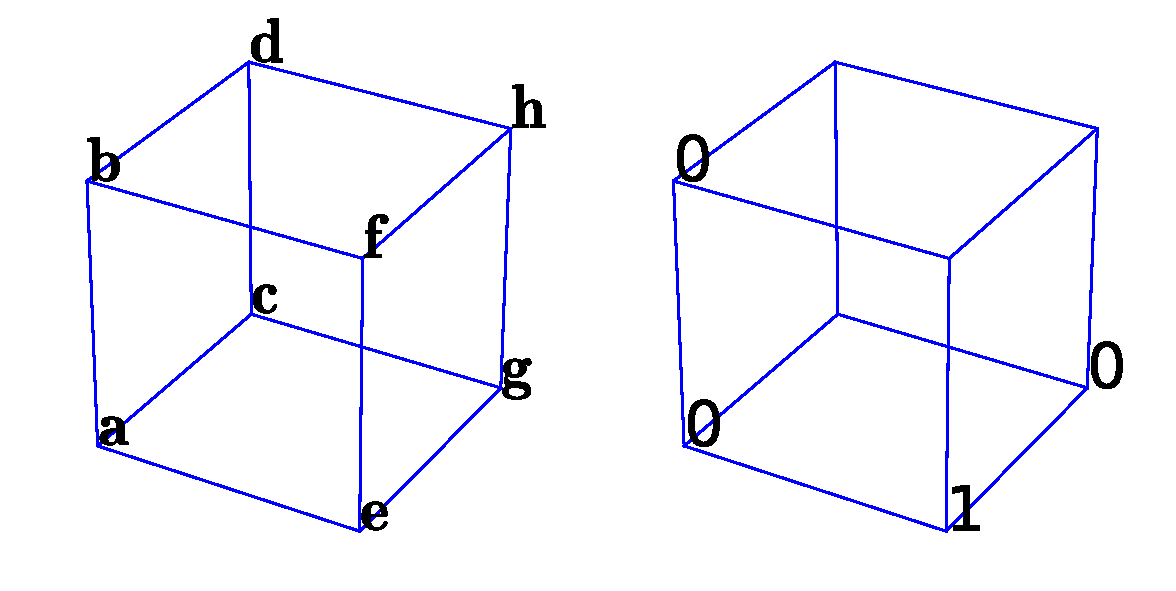
\includegraphics[width=3in]{figures/ae_example.pdf}
  \repeatcaption{FIG:ae_example}{With $S = \Set{\mathbf{a}, \mathbf{b}, \mathbf{d},
  \mathbf{e}}$, we have $\esfs = \Set{\mathbf{c}, \mathbf{f}}$.}
  \label{FIG:ae_example2}
\end{figure}

\begin{table}[t]
  \centering
  $$
  \begin{array}{ccccc}
    \toprule
    \mathbf{b} & \mathbf{d} & \mathbf{a} & \mathbf{g} &  \AD(b_i, d_i, a_i, g_i)\\
    \midrule
    0 & 0 & 0 & 1 &   \textbf{1}\\
    0 & 1 & 0 & 1 &   \textbf{0}\\
    1 & 1 & 0 & 0 &   \textbf{0}\\
    \bottomrule
  \end{array}
  $$
  \caption{$\AD(\mathbf{b}, \mathbf{d}, \mathbf{a}, \mathbf{g}) = 1$.}
  \label{TAB:AD_bdag}
\end{table}



In \cite{BayMicDelIJCAI07}, the authors evaluated this classifier on a Boolean
setting $\mathbb{B}^m$ over 8 benchmarks from the UCI repository.  This
approach led to remarkable results in terms of accuracy, when compared to
off-the-shelf standard classifiers. Nonetheless, this algorithmic description
of the extended classifier does not allow us to grasp its inherent working
behaviour, and it is difficult to extract theoretical properties. The aim of
the next subsection is to give a functional translation of this algorithmic
description.

\subsection{Analogical classifier: a functional definition}
\label{SEC:functional_definition}

As we have previously seen, we can generally assume that
$\AD(\mathbf{a},\mathbf{b},\mathbf{c},\mathbf{d}) \eqdef
\norm{p}{(\mathbf{a}-\mathbf{b})-(\mathbf{c}-\mathbf{d})}$, whether we are
dealing with the arithmetic proportion or the Boolean proportion.
A key observation is that we can formulate this expression with a distance
function on $X^m$. Indeed, a simple rewriting leads to the following expression:
$$\AD(\mathbf{a},\mathbf{b},\mathbf{c},\mathbf{d})=\norm{p}{\mathbf{d} -
(\mathbf{c}-\mathbf{a}+\mathbf{b})}=\norm{p}{\mathbf{d} - \mathbf{d}'},$$
where $\mathbf{d}'\eqdef\mathbf{c}-\mathbf{a}+\mathbf{b}$. Actually,
$\mathbf{d}'$ is nothing but the $4^\text{th}$ vertex of the parallelogram
$\mathbf{a}\mathbf{b}\mathbf{c}\mathbf{d}'$, or equivalently, $\mathbf{d}'$ is
solution of the equation $\mathbf{a}: \mathbf{b} :: \mathbf{c} : \mathbf{x}$.
All this means that $\AD(\mathbf{a},\mathbf{b},\mathbf{c},\mathbf{d})$ simply
is the distance between $\mathbf{d}$ and this $4^\text{th}$ vertex
$\mathbf{d}'$: $\AD(\mathbf{a},\mathbf{b},\mathbf{c},\mathbf{d}) =
\delta_p(\mathbf{d}, \mathbf{d}')$, where $\delta_p$ is the distance defined by
the $p$-norm. Figure \ref{FIG:analogical_dissimilarity} schematically sums up all the aforementioned
properties.  Note that when $(\mathbf{a}, \mathbf{b}, \mathbf{c}) \in S^3$ and
when the associated class equation is solvable, we naturally have $\mathbf{d}'
\in \esf$.
\begin{figure}[!h]
\centering
  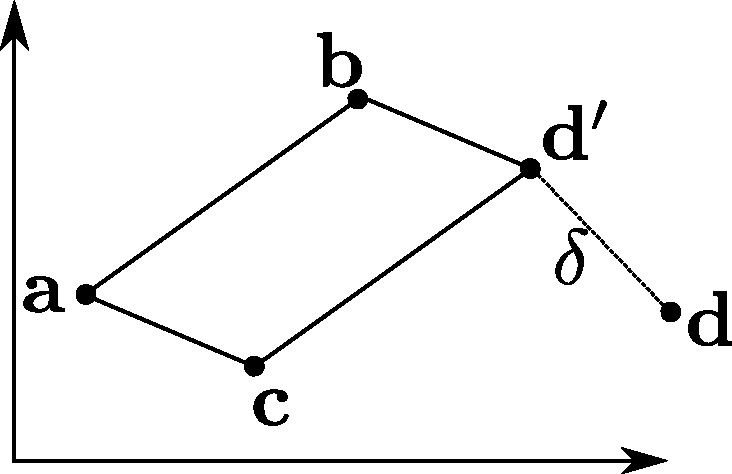
\includegraphics[width=2.5in]{figures/analogical_dissimilarity.pdf}
  \caption{The analogical dissimilarity
  $\AD(\mathbf{a},\mathbf{b},\mathbf{c},\mathbf{d})$ is equal to the distance
  $\delta(\mathbf{d}, \mathbf{d}')$.}
\label{FIG:analogical_dissimilarity}
\end{figure}

\begin{testexample}
Let us consider (again) Figure \ref{FIG:ae_example} on page
\pageref{FIG:ae_example2}. We have already seen that $\AD(\mathbf{b},
\mathbf{d}, \mathbf{a}, \mathbf{g}) = 1$, as proved by Table \ref{TAB:AD_bdag}
  on page \pageref{TAB:AD_bdag}.
We now can reinterpret this statement: $\AD(\mathbf{b}, \mathbf{d}, \mathbf{a},
\mathbf{g})$ should be equal to the distance between $\mathbf{g}$ and another
vector that make up a perfect parallelogram with the $3$-tuple
$(\mathbf{b},\mathbf{d}, \mathbf{a})$. This vector is naturally
$\sol(\mathbf{b},\mathbf{d}, \mathbf{a}) = \mathbf{c}$ and have indeed
$H(\mathbf{c}, \mathbf{g}) =  \AD(\mathbf{b}, \mathbf{d}, \mathbf{a},
\mathbf{g}) = 1$, where $H$ is the hamming distance! The same can be observed
for $\mathbf{h}$: $\AD(\mathbf{a}, \mathbf{b}, \mathbf{e}, \mathbf{h}) =
H(\mathbf{h}, \mathbf{f})$, where $\mathbf{f} = \sol(\mathbf{a}, \mathbf{b},
\mathbf{e})$.
\end{testexample}

We are now finally ready for our unifying functional definition of analogical
classifiers. As we have seen, for a given $\mathbf{x} \in X^m$, Algorithm
\ref{ALGO:extended_classifier} tries to minimize
$\AD(\mathbf{a},\mathbf{b},\mathbf{c},\mathbf{x})$ over all the $3$-tuples
$(\mathbf{a},\mathbf{b},\mathbf{c}) \in S^3$. In the light of what has just
been explained, we see that this is equivalent to finding the closest vertex
$\mathbf{d}' \in \esf$ from $\mathbf{x}$ for any $(\mathbf{a}, \mathbf{b},
\mathbf{c}) \in S^3$. In other words, \textbf{looking for the $k$ $3$-tuples in
$S^3$ that have the smallest value of $\AD$ with $\mathbf{x}$ amounts to
finding the $k$ closest elements to $\mathbf{x}$ in $\esf$}. We will call these
elements the $k$ \textbf{nearest analogical neighbors} of $\mathbf{x}$:

\begin{definition}[The $k$ nearest analogical neighbors]
  \label{DEF:knan}
  For any $\mathbf{x} \in X^m$, and any training set $S \subset X$, we define
  the $k$ nearest analogical neighbors of $\mathbf{x}$ as the set:
  $$k\text{-nan}\left(\mathbf{x}, S\right) \eqdef \Set{\argmin_{\mathbf{d}' \in
  A_E^Y(S)}^k
  \delta(\mathbf{x},\mathbf{d}')},
  $$
  where $\argmin_{\Sigma}^k \delta(\mathbf{x}, \cdot)$ returns the $k$ elements in $\Sigma$
  with the least value of $\delta$.
  Another equivalent way of defining $k\text{-nan}$ is:
  $$k\text{-nan}\left(\mathbf{x}, S\right) \eqdef k\text{-nn}\left(\mathbf{x},
  \esf\right),$$
  where $k\text{-nn}\left(\mathbf{x},\Sigma\right)$ is the set of $k$ nearest
  neighbors of $\mathbf{x}$ in the set $\Sigma$. Ties are broken at random.
\end{definition}

For any $\mathbf{x} \in X^m$, the elements in $\knan(\mathbf{x}, S)$ all belong
to $\esf$, so they all have an analogical label. The prediction
$\hat{f}(\mathbf{x})$ of an extended classifier is thus nothing but the most
frequent analogical label:

\begin{definition}[Extended classifier]
  \label{DEF:extended_classifier}
  Given a training set $S$ with an underlying ground truth function $f$,
  an extended classifier with parameter $k$ sets the prediction of an element
  $\mathbf{x} \in X^m$ as follows:

  $$\hat{f}(\mathbf{x}) \eqdef \text{Mode}\Set{\albl{\mathbf{d}'} | \mathbf{d}'
  \in k\text{-nan}\left(\mathbf{x}, S\right)}.
  $$
\end{definition}

In some sense, an analogical classifier behaves as a $\NN$
classifier\footnote{In the following, $\NN$ and $\NAN$ will denote classifiers.
$\knn$ and $\knan$ denote sets, as in Definition \ref{DEF:knan}.} but
on an extended training set. The above definitions lead us to understand the
process of analogical classification as follows:
\begin{enumerate}
  \item First, extend the training set $S$ to its analogical extension
    $\esf$. $\esf$ can be viewed as an extended training set that has
    \textbf{class noise}: the labels associated with elements in $\esfs$ are
    their analogical labels as defined in Definition
    \ref{DEF:analogical_label}, and they may not be equal to the ground truth
    value $f(\mathbf{x})$.
  \item Then, simply apply a classical $k$-NN strategy over this extended
    training set.
\end{enumerate}

Figure \ref{FIG:extended_classifier} gives an illustration of the classification process for
$k = 1$: the
label of $\mathbf{x} \in X$ is unknown, and we set it to that of $\mathbf{d}'
\in \esf$ (a circle), which is its nearest analogical neighbour. To show that
the analogical label of $\mathbf{d}'$ has itself been inferred, it is depicted
as transparent instead of plain black.
\begin{figure}
\begin{center}
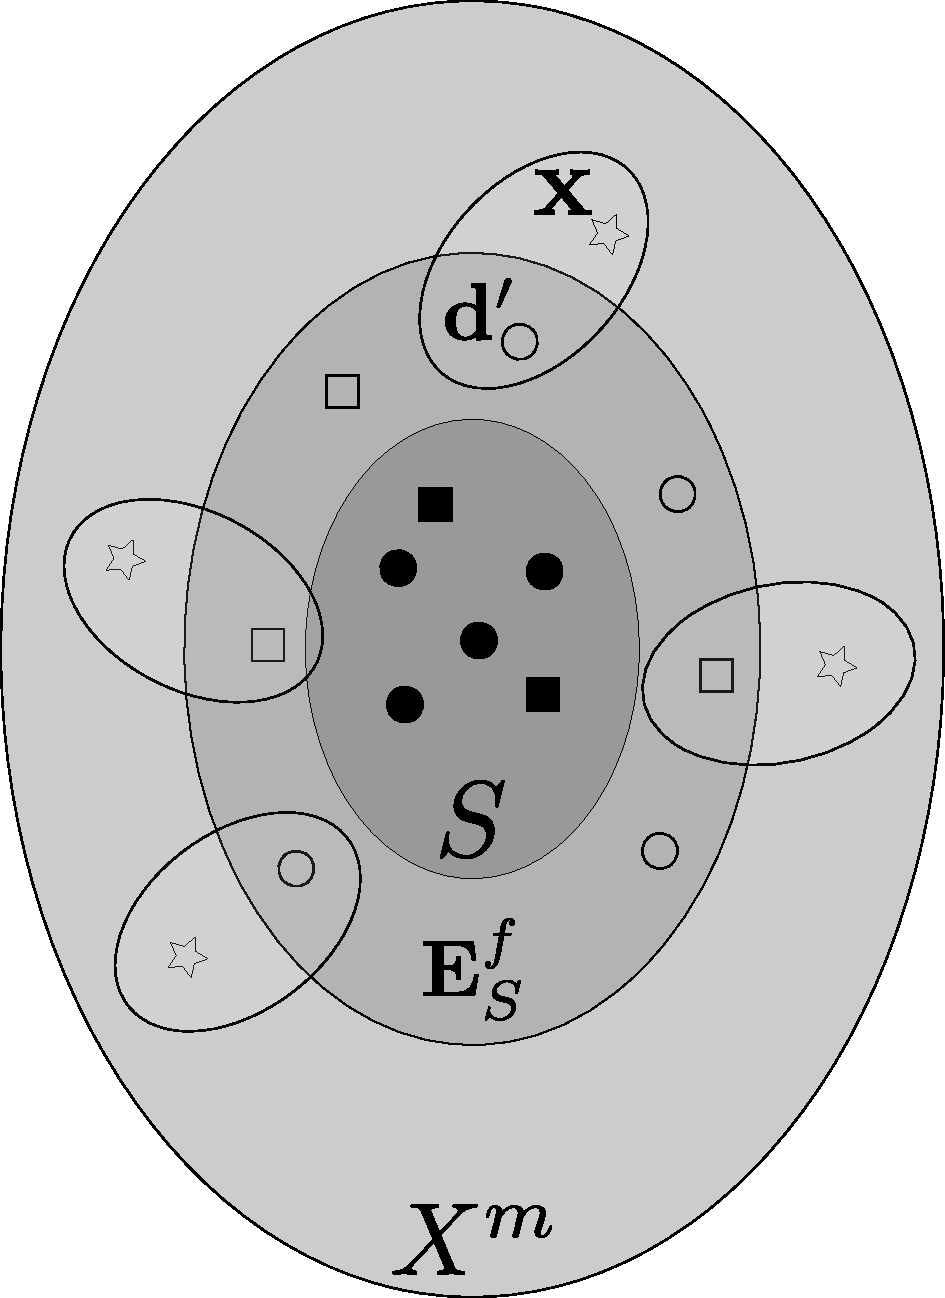
\includegraphics[scale=0.20]{figures/extended_classifier.pdf}
\end{center}
  \caption{Classification process of an extended analogical learner.
  $\hat{f}(\mathbf{x}) = \albl{\mathbf{d}'}$.}
\label{FIG:extended_classifier}
\end{figure}
Let us note that topologically speaking, Figure \ref{FIG:extended_classifier}
is not representative of a real case: even if we always have $S \subseteq \esf
\subseteq X^m$, this does not mean that these sets are embedded into one
another as shown in the drawing. Actually, elements of $S$ (and thus of $\esf$)
are usually scattered over the whole universe.

\begin{testexample}
Going back (for the last time!) to Figure \ref{FIG:ae_example}, our
new functional view allows us to consider the following steps:
\begin{enumerate}
  \item First extend $S = \Set{\mathbf{a}, \mathbf{b}, \mathbf{d}, \mathbf{e}}$
    to $\esf = \Set{\mathbf{a}, \mathbf{b}, \mathbf{c}, \mathbf{d},
    \mathbf{e}}$ with $\hat{f}(\mathbf{c}) = \albl{\mathbf{c}} = 1$ and
    $\hat{f}(\mathbf{f}) = \albl{\mathbf{f}} = 1$.
  \item Then, to classify $\mathbf{g}$, we simply look to its nearest neighbors
    in $\esf$, which are $\mathbf{c}$ and $\mathbf{e}$. The aggregation of
    their analogical labels leads to
    $\hat{f}(\mathbf{g}) = 1$. The nearest neighbors of $\mathbf{h}$ are
    $\mathbf{d}$ and $\mathbf{f}$, which also leads to $\hat{f}(\mathbf{h}) =
    1$.
\end{enumerate}
\end{testexample}

As far as we know, this is the first time a functional definition of
analogy-based classifiers is given. This definition clearly fits with the known
algorithms but obviously, some implementation details cannot be exactly caught
up by such a high level description. It is indeed possible to find a few edge
cases where this functional definition may not output the same result as
algorithm \ref{ALGO:extended_classifier}: this is the case for example when the
nearest analogical neighbor (nan) of $\mathbf{x}$ is not unique. It is also the
case with the Boolean proportion when the closest vertex $\mathbf{d}'$ does not
belong to $\mathbb{B}^m$.  However, as we will see later, these cases are not
likely to occur and the two approaches (that of Algorithm
\ref{ALGO:extended_classifier} and that of Definition
\ref{DEF:extended_classifier}) produce very similar results, thus empirically
validating this functional definition.

Since we now have a clear functional definition of analogical classifiers, we
are in position to examine some general theoretical properties of analogical
learners. This is the purpose of the next section.
\section{Theoretical properties of analogical classifiers}
\label{SEC:theoretical_properties_of_analogical_classifiers}

The functional definition of analogical learners opens the door the study of
various theoretical properties of analogical classifiers, which had only been
described algorithmically so far. Just like for the $k$-NN literature,
theoretical results are easier to derive when $k = 1$. We will therefore mostly
focus on the properties of the 1-NAN classifier.
\subsection{Study of convergence}

Let us consider the case where $X^m=\mathbb{R}^m$, and let $\delta$ be any
distance function defined from a norm. Simply because $S \subseteq \esf$ for
any $S$, the
following inequality holds for any $\mathbf{x} \in X^m$ :
$$\delta(\mathbf{x}, \nan(\mathbf{x},S)) \leq \delta(\mathbf{x},
\nn(\mathbf{x},S)).$$


Now, let us consider  $\mathbf{x}^{(i)}$ an i.i.d. sequence of random variables
in $\mathbb{R}^m$, where $\mathbb{R}^m$ is equipped with a probability measure
denoted $P$. The training set will be denoted $S_n=\Set{\mathbf{x}^{(i)}, ~ i
\in [1, n]}$. As $S_n$ is random, then $\nan(\mathbf{x},S_n)$ can also be
considered as a random element of $X^m$.  We then are in the exactly same
context as the work of Cover \& Hart (\cite{CovHarTIT67}), and we obtain the
same result:
\begin{property}
  \label{PROPER:convergence_nan}
  For any $\mathbf{x}$, its nan $\nanemph(\mathbf{x}, S_n)$ converges almost
  surely towards $\mathbf{x}$ as $n$ tends to infinity:
  $$P\left(\lim_{n \to \infty} \nanemph(\mathbf{x}, S_n) = \mathbf{x}\right) =
  1.$$
\end{property}
\begin{proof}
  The proof can be easily derived from the results of Cover \& Hart in
  \cite{CovHarTIT67}. Indeed, they have already showed that the nearest neighbor of
  $\mathbf{x}$ converges almost surely towards $\mathbf{x}$ as $n$ tends to
  infinity:
  $$P\left(\lim_{n \to \infty} \nn(\mathbf{x}, S_n) = \mathbf{x}\right) =
  1.$$
  To prove this result, they simply start from the fact that
  $\delta(\mathbf{x}, \nn(\mathbf{x}, S_n))$ converges in probability towards
  $0$:
  $$\forall \epsilon > 0,~~P\Big(\delta(\mathbf{x}, \nn(\mathbf{x}, S_n)) >
  \epsilon\Big) = 0.$$
  Using the previous fact that $\delta(\mathbf{x}, \nan(\mathbf{x},S_n)) \leq
  \delta(\mathbf{x}, \nn(\mathbf{x},S_n))$, the convergence in probability of
  $\delta(\mathbf{x}, \nan(\mathbf{x},S_n))$ towards $0$ is immediate. Then, it
  naturally follows that $\nan(\mathbf{x}, S_n)$ converges almost surely
  towards $\mathbf{x}$, following the same steps as Cover \& Hart.
\end{proof}

Let us note the following points:
\begin{enumerate}
\item The result of Cover and Hart was actually proved in a less restrictive
  setting than ours. They have proven their result for any separable metric
    space, without any additional structure. Unfortunately, we are not able to
    follow these lines here, because there is no known way to define an
    analogical dissimilarity on a metric space, without the help of any other
    structure or operator (see \cite{MicBayDelJAIR08} for a detailed discussion
    on this issue).
  \item Cover \& Hart proved that when $n$ tends to infinity, the probability
    of error of the $1$-\NN classifier is less than twice that of the Bayes
    probability of error, and therefore less than twice the probability of error of
    any other classifier. We have not been able to prove such a strong result
    for the $1$-\NAN~classifier, but its probability of error will be thoroughly
    investigated in Subsection \ref{SEC:accuracy_analysis}.
  \item We have to be careful about the interpretation of Property
    \ref{PROPER:convergence_nan} in terms of machine learning. Indeed, another
    key property is proved in \cite{CovHarTIT67}: for an integrable
    function $f$  over $\mathbb{R}^m$ w.r.t. the probability measure $P$, the
    expectation of $f(\nn(\mathbf{x},S_n))- f(\mathbf{x})$ converges to 0 when
    $n$ tends to infinity.  This means that asymptotically, the nearest
    neighbour of $\mathbf{x}$ has the same properties as $\mathbf{x}$, and
    particularly: \textbf{they have the same label}, which is a very powerful
    property when we are dealing with a classification task. Sadly, such a
    property has not been proven for $\nan(\mathbf{x}, S_n)$.
\item Finally, it is clear that when $n$ goes to infinity, the behavior of an
  analogical classifier tends to that of a nearest neighbours classifier.
    Indeed, when $S_n$ is very big, the nearest analogical neighbour of an
    element $\mathbf{x}$ simply is its nearest neighbour, in most cases.
    Moreover, when the nan and the nn are too close, paying the price of the
    noise related to the nan may not be worth it. This supports the common
    acknowledgement that analogical reasoning is mostly useful when very few
    data are available.  In this later case extending a small training set with
    its analogical extension may be particularly beneficial, as we will see in
    Chapter \ref{CHAP:analogy_preserving_functions}.

\end{enumerate}
To conclude this discussion, even if the convergence result is interesting in
itself, it does not say a lot in terms of machine learning. A much more
interesting and powerful theoretical result of analogical classifiers will be
proved in Chapter \ref{CHAP:analogy_preserving_functions}.

\subsection{Vapnik Chervonenkis (VC) dimension}
\label{SEC:VCdim}
The notion of VC-dimension was originally defined by Vapnik and Chervonenkis
\cite{Vap98}, and introduced into learnability theory by Blumer et al.
\cite{BluEhrHauWarACM89}. Roughly speaking, the VC-dimension (denoted VC) of a class of
learners is a numerical measure of their discrimination power. One of the main
results about the VC-dimension is that it allows to bound the true risk $R$ of
a learner. With probability $1 - \eta$, and under some theoretical conditions
that we omit here, we have:

$$R \leq R_{\text{emp}} + \sqrt{\frac{1}{n} \cdot \left[\text{VC}(\log(2n /
\text{VC}) + 1) - \log(\eta/4)\right]},$$
where $R_\text{emp}$ is the probability of error on a training set $S$ of size
$n$, and VC is the VC-dimension of the learner. In our setting,
\begin{itemize}
  \item $R \eqdef P\left(\hat{f}(\mathbf{x}) \neq f(\mathbf{x}) \given[\big]
    \mathbf{x} \in X^m\right)$, and
  \item $R_\text{emp} \eqdef P\left(\hat{f}(\mathbf{x}) \neq f(\mathbf{x})
    \given[\big] \mathbf{x} \in S_n\right)$.
\end{itemize}

This theoretical upper bound on the true risk $R$ is what makes the
VC-dimension of a class of learners an essential element of their theoretical
study. The VC-dimension is defined as follows:

\begin{definition}[VC-dimension]
  \label{DEF:VCdim}
  We consider a class of learners $\mathcal{C}$ and a set $S_n$ of $n$ labeled
  elements in $X^m$. There are exactly $2^n$ ways to label each of the $n$
  elements. If for any labeling, there exist a learner in $\mathcal{C}$ that
  correctly labels all the elements in $S_n$, we say that $\mathcal{C}$
  \textbf{shatters} $S_n$.\\

  The VC-dimension of $\mathcal{C}$ is the biggest $n$ such that there exist a
  set of $n$ points $S_n$ that can be shattered by $\mathcal{C}$.
\end{definition}

%We consider a universe $X$ (usually a Cartesian product to represent the data)
%and a family $\mathcal{H}=\{h_i \subseteq X|i \in I\}$ of subsets of $X$.  The
%elements of $\mathcal{H}$ will be referred as hypothesis or models.  Given a
%subset $A$ of $X$, we can consider the new family of subsets $tr(\mathcal{H},A)
%= \{h_i \cap A \subseteq X|i \in I\}$: this family is called the {\it trace of
%$\mathcal{H}$ over $A$}. This is obviously a subset of the power set of $A$,
%$2^A$ i.e. $tr(\mathcal{H},A) \subseteq 2^A$.  We say that $\mathcal{H}$
%shatters $A$ iff $tr(\mathcal{H},A)=2^A$.  $VC\mbox{-}dim(\mathcal{H})$ is then
%the size of the largest finite subset which can be shattered by $\mathcal{H}$:
%\begin{definition} $VC\mbox{-}dim(\mathcal{H}) = \bigsqcup \{|A| \given[\big]
%  \mathcal{H} \mbox{ shatters } A \}$,
%\end{definition}
%where $\bigsqcup$ is the least upper bound operator.  In the case where
%$\forall n \in\mathbb{N}, \exists  A \subset X, |A|=n \mbox{ such that }
%\mathcal{H} \mbox{ shatters } A$, we simply say that:
%$$VC\mbox{-}dim(\mathcal{H})=\infty.$$ \noindent
%As a binary classifier $c$ over $X$ defines a subset of $X$ with $c^{-1}(1)=\{x
%\in X | c(x)=1\}$, we can associate to a class $\mathcal{C}$ of classifiers a
%family of subsets $\{c^{-1}(1) | c \in \mathcal{C}\}$ and then the
%$VC\mbox{-}$dimension of a set of classifiers is as below:
%\begin{definition}
%$VC\mbox{-}dim(\mathcal{C})=VC\mbox{-}dim(\{c^{-1}(1) | c \in \mathcal{C}\})$
%\end{definition}

Let's first consider the class of nearest neighbors classifiers:
$\mathcal{C}_{\text{NN}}=\{ k\text{-NN classifiers}, k \in \mathbb{N}^*\}$. It
is clear that the VC-dimension of $\mathcal{C}_{\text{NN}}$ is infinite: taking
$k = 1$, any training set of any size can be perfectly labeled by 1-NN,
because every element is its own nearest neighbor. Actually, we can easily show
the same result for the analogical learners.

\begin{proposition}
  \label{PROPOS:VCdim}
  The class $\mathcal{AC}_k$ of analogical learners has infinite VC-dimension.
\end{proposition}
\begin{proof}
  Considering Definition \ref{DEF:extended_classifier} on page
  \pageref{DEF:extended_classifier} with $k = 1$, we see
  that the predicted label of any element $\mathbf{x}$ is that of its nan. For
  any element $\mathbf{x}$ in $S_n$, $\mathbf{x}$ is its own nan (just like
  $\mathbf{x}$ is its own nearest neighbor). Hence, any training set $S_n$ of
  size $n$ is correctly labeled by 1-NAN, and thus can be shattered by
  $\mathcal{AC}_k$. Therefore, the VC-dimension of $\mathcal{AC}_k$ is infinite.
\end{proof}

Clearly, the upper bound is a decreasing function in $n$, and an increasing
function in the VC dimension of the learner. As such, we usually want the
VC-dimension of our classifiers to be small. However, we have previously seen
that the nearest neighbors classifiers, despite their infinite
VC-dimension, enjoy many interesting theoretical properties, and their
practical efficiency is well-acknowledged. In fact, the upper bound on the true
risk does not even hold for classes of learner whose VC-dimension is infinite
\cite{Bur98}. We then need to keep in mind that even though the analogical
learners have an infinite VC-dimension, which is an interesting result in its
own right, this does not necessarily prevent them from being useful
classifiers.

\subsection{Accuracy analysis}
\label{SEC:accuracy_analysis}

In this section, we study the accuracy of an analogical classifier, and more
particularly that of the $\NAN$ classifier. As explained in Section
\ref{SEC:functional_definition}, for a given $\mathbf{x} \in X^m$ and a
training set $S \subset X^m$, the prediction $\hat{f}(\mathbf{x})$ is set as:
$$
\hat{f}(\mathbf{x}) ~ \eqdef ~ \albl{\nan(\mathbf{x}, S)} ~ \eqdef ~ \albl{\nn(\mathbf{x}, \esf)}.
$$

We now equip the set $X^m$ with a probability distribution denoted $P$.  The
accuracy of the $\NAN_S$ classifier\footnote{The $S$ subscript is here to
specify that the training set of the $\NAN$ algorithm is $S$. The same notation
is used for the \textit{nearest neighbour} algorithm: $\NN_\Sigma$ is the $\NN$
algorithm trained on the set $\Sigma$.} over all the elements of $X^m$ is
defined as:
$$\acc(\NAN_S, X^m)\eqdef P\left(\hat{f}(\mathbf{x})=f(\mathbf{x}) \given[\big]
\mathbf{x} \in X^m\right).$$
Our main result is given by Proposition \ref{PROPOS:accuracy_nan}:
\begin{proposition}
  \label{PROPOS:accuracy_nan}
  The accuracy of $\NAN_S$ over $X^m$ can be seen as the weighted sum of the
  accuracy of $\NN$ over $A$ and $B$, using a different training set each time
  (respectively $S$ and $\esfs$):
  \begin{align*}
    \acc(\NAN_S, X^m) = ~&\acc(\NN_S, A) \cdot \alpha ~ + \\
                        &\acc(\NN_{\esfs}, B) \cdot (1 - \alpha),
  \end{align*}
  where:
  \begin{itemize}
  \item $A \eqdef \set{\mathbf{x} \in X^m | \nan(\mathbf{x}, S) \in S}$: the
    elements that have their nan in $S$.
  \item $B \eqdef \set{\mathbf{x} \in X^m | \nan(\mathbf{x}, S) \in \esfs}$: the
    elements that have their nan in $\esfs$.
  \item $\alpha \eqdef P(\mathbf{x} \in A)$ and $1 - \alpha = P(\mathbf{x} \in
    B)$. 
  \end{itemize}
  Naturally, $A \cup B = X^m$ and $A \cap B = \varnothing$.
\end{proposition}
\begin{proof}
By observing that for any $\mathbf{x}$, its $\nan$ either belongs to $S$ or to
$\esfs$, the accuracy $\acc(\NAN_S, X^m)$ can be split into two distinct parts as follows:

\begin{align*}
  &\acc(\NAN_S, X^m) \eqdef P\left(\hat{f}(\mathbf{x})=f(\mathbf{x}) \given[\big] \mathbf{x} \in
  X^m\right) = P\left(\albl{\nan(\mathbf{x}, S)} = f(\mathbf{x})\right)\\
  =~&P\left([\albl{\nan(\mathbf{x}, S)} = f(\mathbf{x}) ]\wedge
  [\nan(\mathbf{x}, S) \in S ] \right)~ +
  P\left([\albl{\nan(\mathbf{x}, S)} = f(\mathbf{x})] \wedge [\nan(\mathbf{x},
  S) \in \esfs]\right)\\
  =~&P\left([\albl{\nn(\mathbf{x}, \esf)} = f(\mathbf{x})] \wedge
  [\nn(\mathbf{x}, \esf) \in S ]\right)~ +
  P\left([\albl{\nn(\mathbf{x}, \esf)} = f(\mathbf{x})] \wedge
  [\nn(\mathbf{x}, \esf) \in \esfs]\right) \\
  =~&P\left([\albl{\nn(\mathbf{x}, \esf)} = f(\mathbf{x})] \given[\big]
  [\nn(\mathbf{x}, \esf) \in S ]\right) \times
  P\left([\nn(\mathbf{x}, \esf) \in S]\right) ~+ \\
  &P\left([\albl{\nn(\mathbf{x}, \esf)} = f(\mathbf{x})] \given[\big]
  [\nn(\mathbf{x}, \esf) \in \esfs]\right) \times
  P\left([ \nn(\mathbf{x}, \esf) \in \esfs]\right)
\end{align*}

Let us denote  $\alpha \eqdef P\left(\nn(\mathbf{x}, \esf) \in S\right)$.
Obviously, we also have $\alpha \eqdef P\left(\nan(\mathbf{x}, S) \in
S\right)$.  The above formula becomes:
\begin{align*}
  &\acc(\NAN_S, X^m) = \\&P\left([\albl{\nn(\mathbf{x}, \esf)} = f(\mathbf{x})]
  \given[\big] [\nn(\mathbf{x}, \esf) \in S] \right) * \alpha ~+ \\
  &P\left([\albl{\nn(\mathbf{x}, \esf)} = f(\mathbf{x})] \given[\big]
  [\nn(\mathbf{x}, \esf) \in \esfs]\right) * (1 - \alpha).
\end{align*}

Let us focus on the first term, temporarily discarding the factor $\alpha$:
$$P\left([\albl{\nn(\mathbf{x}, \esf)} = f(\mathbf{x})] \given[\big]
[\nn(\mathbf{x}, \esf) \in S] \right).$$

It is easy to see that the event $[\nn(\mathbf{x}, \esf) \in S]$ is equivalent
to the event $[\nn(\mathbf{x}, \esf) = \nn(\mathbf{x}, S)]$. As a result, we
can transform the first term to get a better grasp of its meaning:
\begin{align*}
  &P\left([\albl{\nn(\mathbf{x}, \esf)} = f(\mathbf{x})] \given[\big]
  [\nn(\mathbf{x}, \esf) \in S] \right)\\
  =~ &P\left([\albl{\nn(\mathbf{x},\esf)} = f(\mathbf{x})] \given[\big]
  [\nn(\mathbf{x}, \esf) = \nn(\mathbf{x}, S)]\right)\\
  =~ &P\left([\albl{\nn(\mathbf{x}, S)} = f(\mathbf{x})] \given[\big]
  [\nn(\mathbf{x}, \esf) \in S]\right).
\end{align*}

In this form, the first term is just the accuracy of the $\NN_S$ algorithm over
the elements that have their nearest analogical neighbour in $S$.
As for the second term, the same process can be applied by observing that the
event $[\nn(\mathbf{x}, \esf) \in\esfs]$ is equivalent to the event
$[\nn(\mathbf{x}, \esf) = \nn(\mathbf{x}, \esfs)]$. This leads to
\begin{align*}
  &P\left([\albl{\nn(\mathbf{x}, \esf)} = f(\mathbf{x})] \given[\big]
  [\nn(\mathbf{x}, \esf) \in \esfs]\right)\\
  =~ &P\left([\albl{\nn(\mathbf{x}, \esfs)} = f(\mathbf{x})] \given[\big]
  [\nn(\mathbf{x}, \esf) \in \esfs]\right).
\end{align*}

This second term is then the accuracy of the $\NN_{\esfs}$ algorithm over the
elements that have their nearest analogical neighbour in $\esfs$.

In the light of these interpretations, we can directly rewrite the accuracy
formula in a the concise form given in Proposition \ref{PROPOS:accuracy_nan}.
\end{proof}

The value $\acc(\NN_S, A)$ is the accuracy of $\NN_S$ over all the elements in
$A$. A theoretical study of this accuracy has been done in \cite{LanIbaIJCAI93}
when the size of $A$ is known.  Regarding $\acc(\NN_{\esfs}, B)$, this is the
accuracy of $1$-$\NN$ when the training set is
noisy, and has been studied in \cite{OkaYugIJCAI97}. This last formula leads
to the consistent facts:
\begin{enumerate}
\item The smaller $\esfs$ (i.e. analogical reasoning does not
  bring much more labels), the closer $\alpha$ is to $1$, the closer $A$ is to
  $X^m$ and the more the accuracy of $\NAN_S$ tends towards the accuracy of
  $\NN_S$ over $X^m$.
\item In return, if $\esf$ is much bigger than $S$, $\alpha$ is then small, $B$
  is close to $X^m$ and the accuracy of $\NAN_S$ greatly depends on the quality
  of $\esf$:  \end{enumerate}

\begin{definition}[Quality of the analogical extension $\omegasf$]
  \label{DEF:omega}
  Given a training set $S\subset X^m$ and a ground truth function $f$, the
  \textbf{quality} of the analogical extension $\esf$ is defined as:
  $$
  \omegasf \eqdef P\left(\albl{\mathbf{x}} = f(\mathbf{x}) \given[\big]
  \mathbf{x} \in \esfs\right).$$
  Note that the value $1 - \omegasf$ corresponds to the class noise of $\esfs$.
\end{definition}

This closes our contributions to the theoretical properties of analogical
classifiers. In the next section, we empirically investigate and illustrate the
soundness of our results.

\section{Experiments and empirical validation}
\label{SEC:experiments_and_empirical_validation}
In order to get an empirical validation of our formulas, we have developed a
set of experiments that we now describe.

\subsection{Evaluation protocol}

Working with Boolean vectors, we have computed the accuracies of the 1-\NAN~and
1-$\NN$~ algorithms over $X=\mathbb{B}^m$ for $m = 8$. Other values of $m$ have
been investigated, leading to very similar results.  The ground truth label of
the elements of $X^m$ is defined by different Boolean functions $f$:
\begin{itemize}
\item $f_1(\mathbf{x})=x_i$ for some $i$. These functions are called
  projections, or dictators.  They lead to perfectly linearly
    separable problems, i.e.  there exist an hyperplane that can perfectly
    discriminate both classes. As such, they are expected to be fairly easy to
    learn.
  \item $f_2(\mathbf{x})= \bigoplus_{i = 1}^k  x_i$ for some $k \in[1, m]$, where $\oplus$
    is the XOR operator (which is associative). These functions
    lead to highly non-linearly-separable problems: remember the example of
    Figure \ref{FIG:classification_problem} on page
    \pageref{FIG:classification_problem}, who was an instance of a XOR problem.
    XOR problems are traditionally difficult to learn.
  \item $f_3(\mathbf{x})= \bigwedge_{i = 1}^k  x_i$ for some $k \in [1, m]$.
  \item $f_4(\mathbf{x})= \bigvee_{i = 1}^k  x_i$ for some $k\in [1, m]$.
  \item $f_5(\mathbf{x}) = \left[\sum_{i = 1}^m x_i \geq k\right]$ for some $k
    \in [1, m]$, where the function $[\text{cond}]$ is equal to $1$ if cond is
    verified and $0$ else. Simply put, $f(\mathbf{x}) = 1$ iff at least $k$
    components are equal to $1$.
  \item $f_6(\mathbf{x}) = \left[\sum_{i = 1}^m x_i = k\right]$ for some $k
    \in [1, m]$. Simply put, $f(\mathbf{x}) = 1$ iff exactly $k$ components
    are equal to $1$.
\end{itemize}


Regarding the size of the training set, to be sure to fit with the size of the
universe, we have investigated various sizes between $3$ and $100$. When
dealing with a training set of size $100$, the cubic complexity of the
analogical classifier leads to explore a set of approximately $100^3$ elements:
as a consequence, we limit our investigation to a maximum of 100 elements in
the training set in order to get realistic execution time.

All the accuracy (and other metrics) computations are averaged over a set of
100 experiments. We have made sure that the class distributions of the training
sets are as close as possible to that of the whole universe $X^m$.  Note that
our implementation of the $\NAN$ algorithm is not that of algorithm
\ref{ALGO:extended_classifier}, but is instead that of the functional
definition of the analogical classifier as described in Definition
\ref{DEF:extended_classifier}: we first construct the analogical extension set
of $S$, and then proceed to a nearest neighbour strategy over this noisy
extended training set. We have estimated probabilities by frequencies, thus
implicitly assuming a uniform distribution on $X^m$.

For each experiment, we have computed the following measures to empirically
investigate the behaviour of the analogical classifier, and assess our
theoretical results:
\begin{itemize}
  \item The empirical accuracy of the 1NAN classifier, defined\footnote{We
    notice here that $\mathbf{x}$ is only required to belong to $X^m \setminus
    S$ and not to $X^m$, because classifying elements in $S$ is pointless.}
    as\\
    $\acc(\NAN_S) \eqdef P\left(\hat{f}(\mathbf{x}) = f(\mathbf{x})
    \given[\big] \mathbf{x} \in X^m \setminus S \right)$.
  \item The empirical accuracy of the 1NN classifier, which definition is of
    course the same but this time $\hat{f}$ is the output of the 1NN
    classifier.
  \item The \textbf{theoretical} accuracy of 1NAN, as defined in Proposition
    \ref{PROPOS:accuracy_nan}. The probability $\alpha \eqdef P(\mathbf{x} \in
    A$) has been estimated by the frequency $\frac{\mid A \mid}{\mid X^m
    \mid}$. Both sets $A$ and $B$ are easy to determine.
  \item The quality of $\esf$, measured by $\omegasf$ as previously defined in
    Definition  \ref{DEF:omega}. $\omegasf$ has been estimated by the
    frequency $\frac{\big| \Set{\mathbf{x} \in \esfs | \albl{\mathbf{x}} =
    f(\mathbf{x}}\big|}{\big| \esfs \big|}$.
  \item Finally, the quantity $\gamma_S^f \eqdef P(\mathbf{x} \in \esf)$,
    estimated by $\frac{\mid \esf\mid}{\mid X^m \mid}$: the size of the
    analogical extension with respect to that of the whole universe.
\end{itemize}

It is fairly easy to see that both functions $f_1$ and $f_2$ split the universe $X^m$ into
two disjoint sets of size $2^{m - 1}$: those for which $f(\mathbf{x})$ is
equal to $1$, and those with labels equal to $0$. We say that the datasets are
balanced. However, the other functions may lead to very unbalanced datasets. An
extreme case is for example $f_3$ with $k = m$, which leads to $f_3(\mathbf{x})
= x_1 \wedge x_2 \wedge \cdots \wedge x_m$. The only element whose label is $1$
is the vector $\mathbf{x} = (1, 1, \cdots, 1)$. For these very unbalanced
datasets, the accuracy of a classifier is not a relevant measure: predicting
$0$ all the time would lead to an accuracy of almost $1$, but would
systematically assign the wrong label to   $(1, 1, \cdots 1)$. Therefore, as
accuracy is our main concern here, we will focus on functions for which
datasets are as balanced as possible.

In addition to these Boolean functions, we have also run the $\NAN$ algorithm
over the Monk datasets over the UCI
repository\footnote{\url{https://archive.ics.uci.edu/ml/datasets/MONK's+Problems}}.
They are datasets of 432 binarized elements, among which exactly 169 of them
have been used for training.

\subsection{Comments and discussion}

Our experiments are summed-up by Figure \ref{FIG:nan_vs_nn} on page
\pageref{FIG:nan_vs_nn}. As they are the result of multiple averaged
experiments, the measures $\omegasf$ and $\gamma_S^f$ are here denoted $\omega$
and $\gamma$. Paying careful attention to these plots will allow us to draw
interesting conclusions about the behaviour of the 1-NAN algorithm.

\begin{figure}[!h]
\centering
  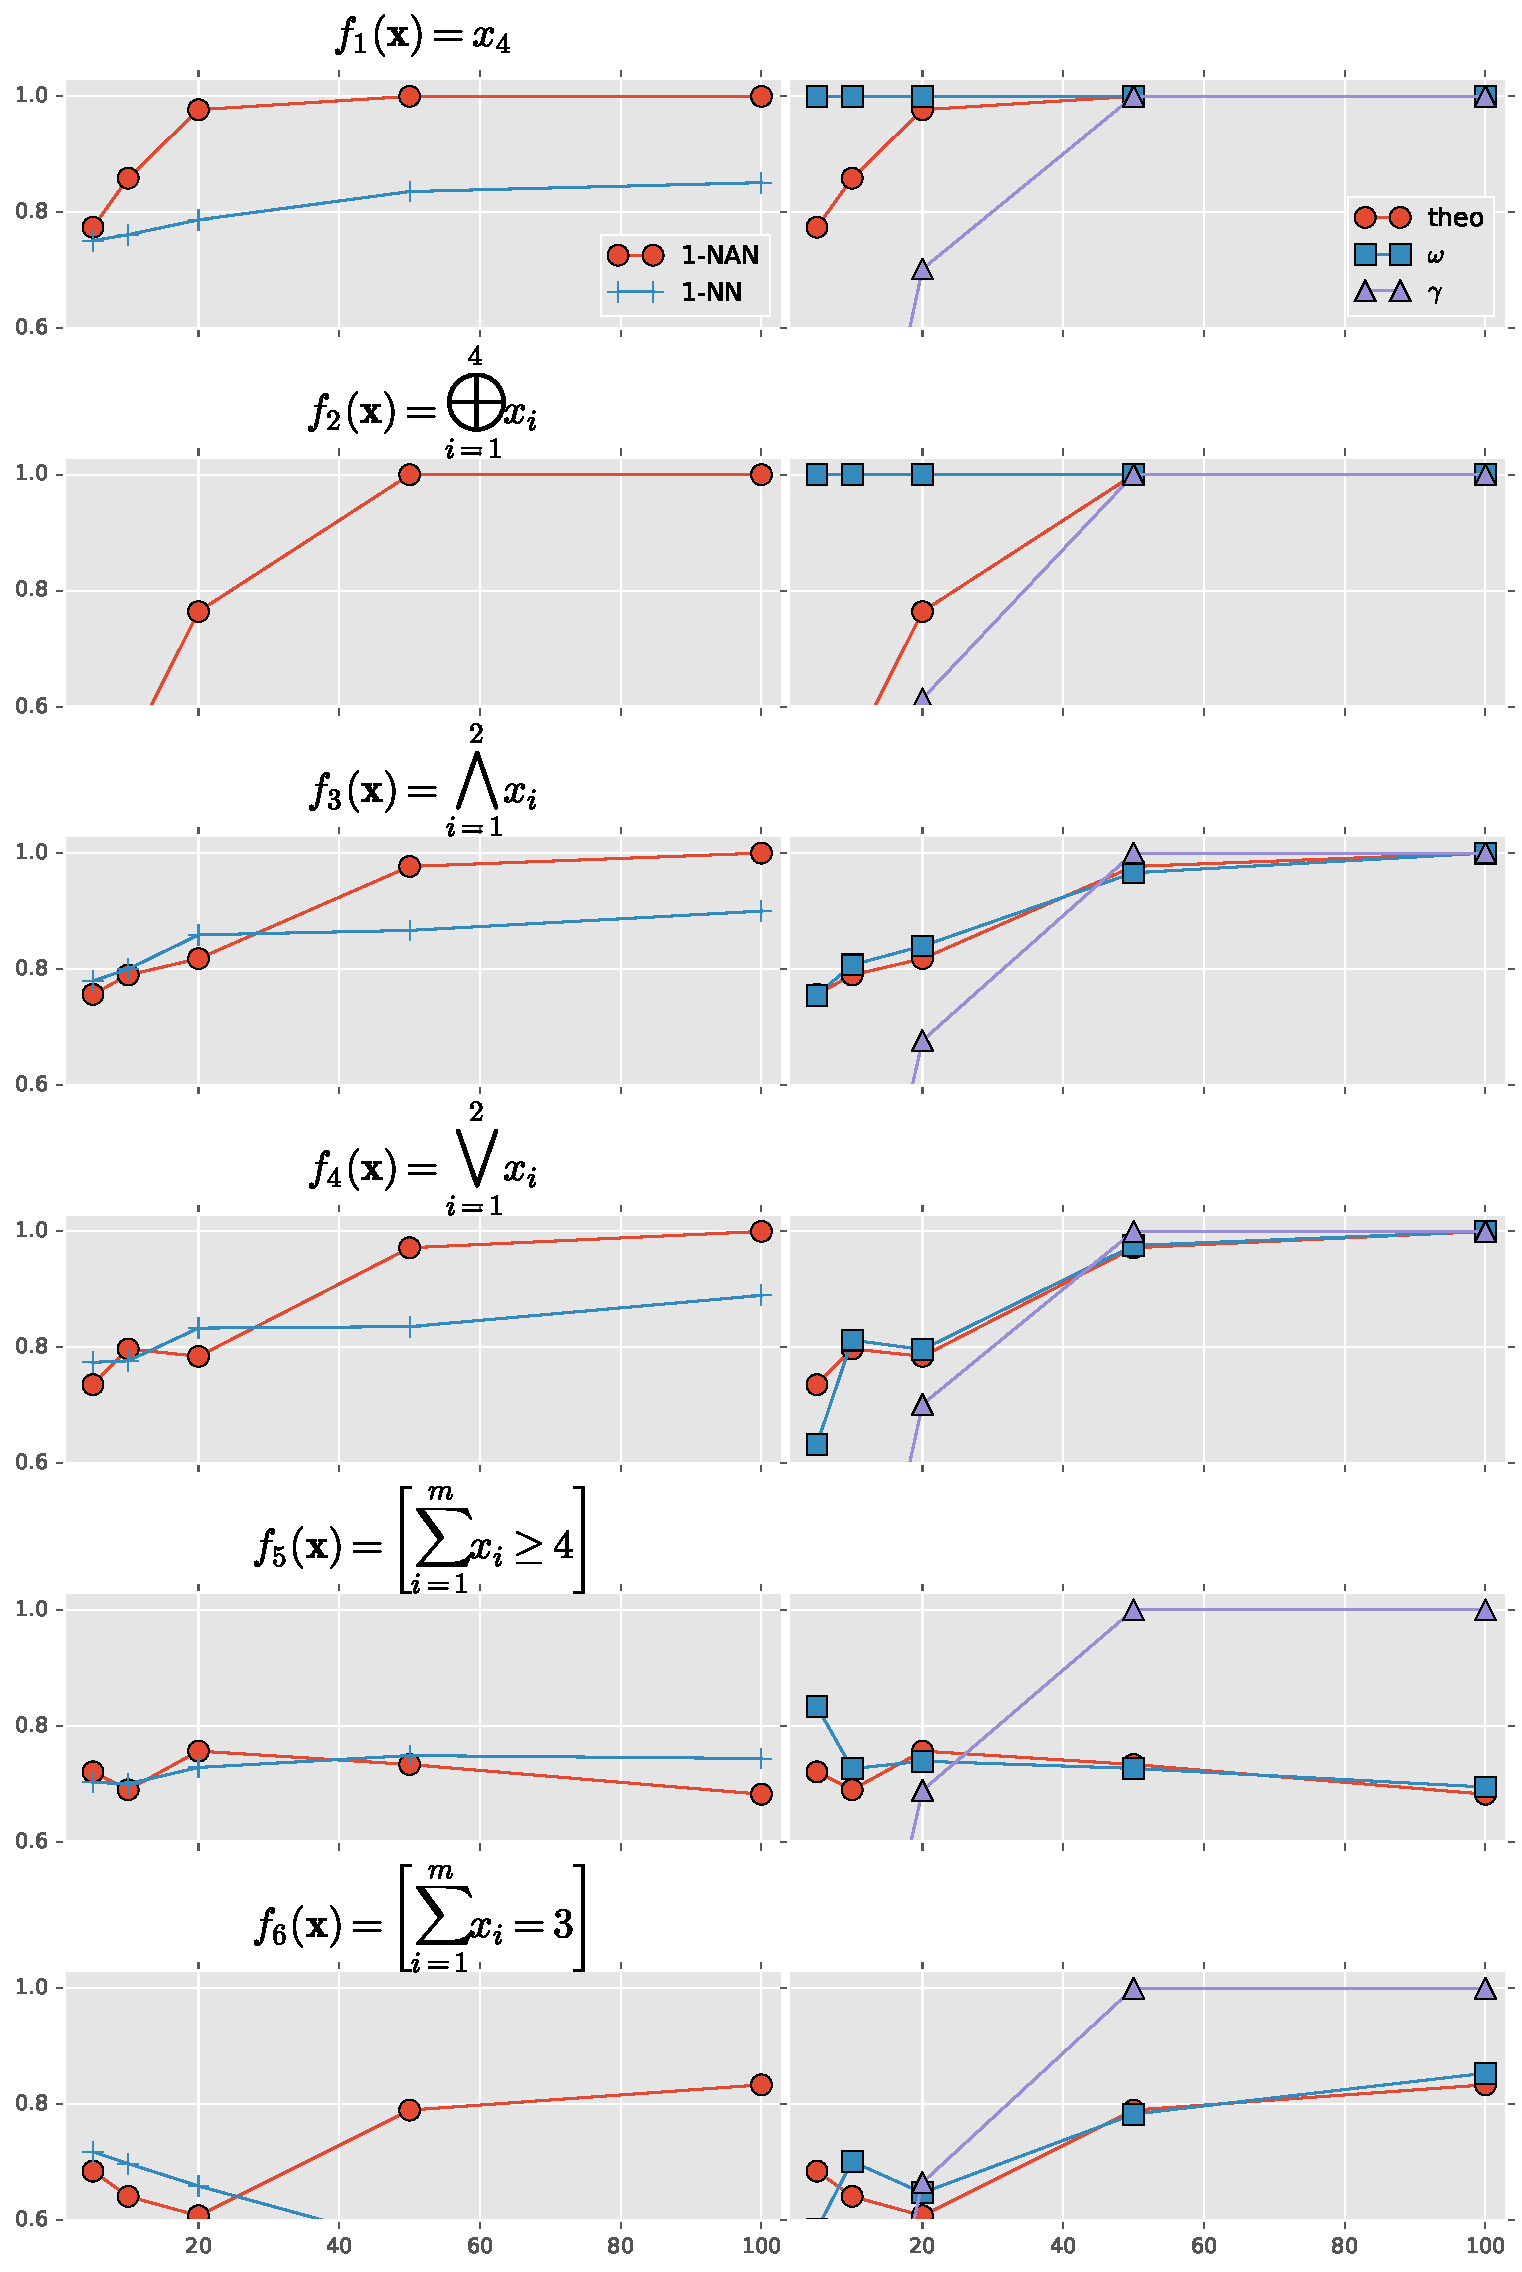
\includegraphics[scale=.50]{figures/nan_vs_nn_SUMMARY_dim8_nexp15.pdf}
  \caption{Accuracies (left) of the 1-NAN and 1-NN algorithms over different
  Boolean functions ($m = 8$) and training set sizes, with corresponding values
  of $\omega$, $\gamma$, and theoretical accuracy (right). The $x$ axis
  corresponds to the size of the training set.}
\label{FIG:nan_vs_nn}
\end{figure}

First, the theoretical accuracy seems to fit perfectly with the empirical
accuracy of the $\NAN$ algorithm, thus validating our theoretical study that
led to proposition \ref{PROPOS:accuracy_nan}. Actually, the maximal difference
we observed between the theoretical accuracy and its actual value is of about
$10^{-10}$.

An interesting observation is that the value of $\omega$ seems to always
converge to that of the theoretical accuracy (and therefore to the actual
accuracy) of $\NAN$. This can be easily explained by paying attention to the
value of $\gamma$, the proportion of elements of $X^m$ that belong to $\esf$.
We see that in any setting, $\gamma$ converges to 1 as $\mid S \mid$ grows.
This means that when $\mid S \mid$ is big enough (but not necessarily
\textit{that} big with respect to $X^m$), the analogical extension of $S$
covers the whole universe $X^m$ (obviously, the bigger the dimension $m$, the
slower the convergence occurs): every element $\mathbf{x}$ is then its own
nearest analogical neighbour and $\hat{f}(\mathbf{x}) = \albl{\mathbf{x}}$. It
is therefore straightforward to see that in this case,
$$
  \omega \eqdef P\left(\albl{\mathbf{x}} = f(\mathbf{x}) \given[\big]
  \mathbf{x} \in \esfs\right) = P\left(\hat{f}(\mathbf{x}) = f(\mathbf{x})
  \given[\big] \mathbf{x} \in \esfs\right)\\ = \acc(\NAN_S, \esfs).
$$
When $\gamma = 1$, the only elements $\mathbf{x}$ we want to classify belong to
$\esfs$ (otherwise they would be in $S$), so this last term exactly corresponds
to the accuracy of the classifier. Another way to see it is to observe that the
first term of the expression of Proposition (\ref{PROPOS:accuracy_nan})
$\acc(\NN_{S}, A) \cdot \alpha$ is zero
because $\alpha = 0$. Only the second term $\acc(\NN_{\esfs}, B) \cdot (1 -
\alpha)$ is of importance, and its value corresponds to $\omega$. As expected,
this observation allows us to state that estimating the value of $\omega$ is
paramount to have a precise idea of the accuracy of an analogical classifier.
%We will provide in the next subsection a method to accurately estimate this
%quantity $\omega$ with the only help of the training set $S$.

A striking result of the experiments is that for the two functions
$f_1(\mathbf{x}) = x_4$ and $f_2(\mathbf{x}) = x_1 \oplus \cdots \oplus x_4$,
the analogical labels are always correctly predicted: $\omega = 1$, i.e. there
is no class noise. However, the accuracy of 1-NAN is not necessarily equal to
$1$ especially for $f_2$ with small training set sizes. The reason is simple:
even if all the elements in $\esf$ are correctly classified, $\esf$ does not
cover the whole space ($\gamma < 1$) so the accuracy of 1-NAN still depends on
that of 1-NN. While the accuracy of 1-NN over $f_1$ is not too bad, the one
over $f_2$ is absolutely terrible and actually below $0.3$ (a random prediction
would have done better!). This is one of the distinguishing features of the XOR
functions: the nearest neighbor of an element is almost always in a different
class, as can be seen on Figure \ref{FIG:classification_problem} (page
\ref{FIG:classification_problem}). So sadly, the 1-NN algorithm can do nothing
but wrong on these kind of functions. In Chapter
\ref{CHAP:analogy_preserving_functions}, we will prove a strong result showing
that both the projections (like $f_1$) and the XOR functions (like $f_2$)
\textbf{always} lead to perfectly sound extensions, for any training set of any
size.

Table \ref{TAB:monks} shows the same metrics for the Monk datasets and also
reports the results of the Analogical Proportion Classifier (\textit{APC}) from
\cite{MicBayDelJAIR08}, which corresponds to algorithm
\ref{ALGO:extended_classifier} with $k=100$.
\begin{table}
\centering
\begin{tabular}{ l  c  c c  c  c }
\toprule
& 1-NAN  & APC & 1-NN  &  $\omegasf$ & $\gamma_S^f$ \\
\midrule
Monk 1 & .961 & .98 & .787 &   .961    &   1 \\
Monk 2 & .998 & 1 & .738 &    .998    &   1 \\
Monk 3 & .963 & .96 & .829 &   .963    &   1 \\
\bottomrule
\end{tabular}
\caption{Accuracies of the 1-NAN, APC and 1-NN algorithms over the Monk
  datasets.}
  \label{TAB:monks}
\end{table}
We note that the functional $\NAN$ approach (almost) achieves the same results
as the somewhat more complex algorithm described in Section
\ref{SEC:extended_classifier}, and that here again the analogical extension set
covers the whole universe: this means that a conservative approach would have
been sufficient! Actually, this raises the following question: why would we
want to look for more than one analogical neighbour when every element of the
universe is already in $\esf$, and therefore \textit{analogically linked} to
those in $S$? Our experiments tend to show that this becomes superfluous,
provided that the training set is big enough.

%\subsection{Estimation of the prediction accuracy}
%
%We have seen in the previous subsection that the value $\omega$ is that of the actual
%accuracy of an analogical classifier when $S$ is big enough. This leads to the
%following question: how can we get a precise estimation of this value $\omega$
%? Answering this would allow us to have a very precise idea of the accuracy we
%can expect from our classifier.
%
%The method we propose for estimating $\omega$ only relies on the training set $S$
%and is very simple: it consists of applying the conservative algorithm to all
%the elements of $S$, and compute the fraction of these elements that have been
%correctly classified. A small yet important modification to the algorithm needs
%to be added: we only want to construct analogical proportions of the form $a :
%b :: c : x$ where $a$, $b$, $c$ and $x$ are all distinct elements. Indeed, the
%proportions $x : x :: x : x$ and $x' : x :: x' : x$ are always true, and the
%solution label related to these proportions would bias the final majority vote
%procedure in a significant way towards the real label $\dot{x}$.
%
%We have applied this estimation protocol to all of the Boolean settings we have
%considered, and it has shown to be very accurate. Figure \ref{omegaplots}
%illustrates a few of these settings (already considered in Figure \ref{plots}).
%\begin{figure}
%  \caption{Values of $\omega$ and its estimation $\hat{\omega}$ for $f_1$, $f_2$ and $f_3$ in
%  $\mathbb{B}^{10}$.}
%\label{omegaplots}
%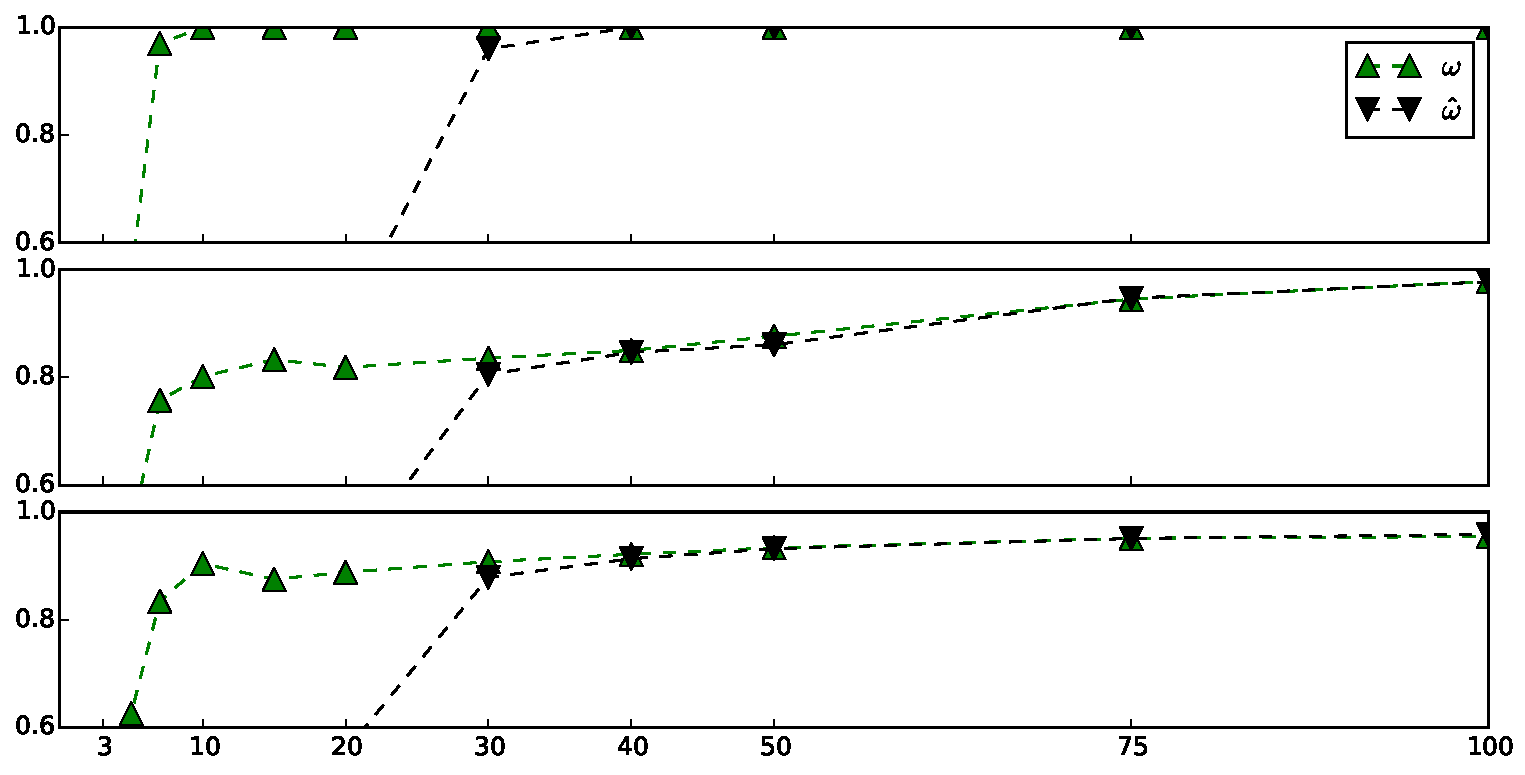
\includegraphics[width=\linewidth]{figures/ecai_estimation_omega.pdf}
%\end{figure}
%We can see that the estimation $\hat{\omega}$ converges to $\omega$ when $S$ is
%big enough. For small values of $S$, this estimation is indeed imprecise as it
%is difficult to find a lot a 3-tuples such that an analogical proportion holds
%for every element.

\section*{Conclusion}

In this Section, we have provided a functional and unifying definition of
analogical learners, which turned out to be closely related to the $k$-NN
classifiers. Starting from this definition, we were in a position to
prove an analytical convergence result, similar to that of the nearest neighbour
algorithm. Obviously, this is not enough to conclude regarding the predictive
ability of analogy-based classifiers. We have also shown that their
VC-dimension is infinite. It should not come as a surprise, as a very
particular case of analogical rule (when the analogical proportion is trivial)
is the $k$-NN rule.

This fact obviously has a consequence on the way we can
work to improve analogy-based classifier.  Indeed, learning by analogy is prone
to over-fitting and a relevant learning strategy should take this fact into
account.  Nevertheless, we have to keep in mind that the VC-dimension
alone is not a perfect marker of the quality of a machine learning algorithm,
especially when it comes to practical implementation.

In terms of accuracy in a Boolean setting, we have found a strong link between
the accuracy of the NAN algorithm and that of the NN algorithm. Our functional
definition tells us that we can consider the NAN algorithm as a NN strategy on an
extended and noisy training set: the analogical extension $\esf$. This leads us
to consider analogical classification as a two-steps process:
\begin{itemize}
  \item First, the training set is extended to the analogical extension
  \item Then, a $k$-NN algorithm is used on this extended training set.
\end{itemize}
Obviously, the accuracy of the NAN algorithm depends on the quality of the
analogical extension. In Chapter \ref{CHAP:analogy_preserving_functions}, we
will entirely describe the conditions needed for this extension to be perfectly
sound.

We have to remember that analogical reasoning brings its whole power in the
case where few data are available. If a lot of data are available, it is very
likely that we have elements similar to the one at hand and, in that case, a
$k$-NN style reasoning is natural. In the opposite case, when we only have a
few relevant cases at hand, applying analogical proportion-based predictions
appears to be a meaningful option.

This concludes for now our investigations with analogical classifiers. We have
seen that they have so far mostly been used for natural language processing
tasks, or classification in Boolean settings. One of the main goal of this
thesis was to apply analogical proportion-based reasoning to concrete,
real-world applications. We have chosen to investigate the suitability of
analogical proportion in the design of recommender systems. This is the object
of the next two chapters.


\chapter{Recommender systems}

In a world of information overload, automatic filtering tools are essential to
extract relevant information from basic noise. In the field of e-commerce,
recommender systems play the role of search engines when surfing the entire
web: they filter available items to provide relevant suggestions to customers.

With the huge development of online businesses, recommender systems have become
more and more popular \cite{RecoSystemHandbook,AdoTuzIEEE2005}. They help to
answer questions as diverse as ``what movie to rent?", ``what item to buy?" or
``which restaurant to try?", but also such as ``what piece of code to
investigate ?" in the case of recommender system for software development.
They do so by providing the user with a list of recommendations.  Obviously,
the more personalized the recommendations, the better the system.  For
instance, a system recommending only the most popular items is useless as it is
likely that the standard customer knows these items. But the maximization of
business profit may also lead to suggest items which are not very popular (and
thus difficult to sell), provided they may be of interest for the user.

A very common way of providing personalized recommendations to a target user is
to estimate its taste for the items that the system provides. The taste of a user
$u$ for a given item $i$ is usually represented as a rating that $u$ would give
to $i$.  The scale of the ratings may vary, but the integer interval [1, 5] and
the \textit{like}/\textit{dislike} scales are very common in real world
systems.

Once these estimations are made, a simple option is to recommend the items with
the highest ratings among all the estimated scores for the considered user
(using the implicit assumption that a user should be interested in the items
with high scores).

Providing an accurate measure of the overall quality of a recommender system is
not a simple task and diverse viewpoints have to be considered (see
\cite{RecoSystemHandbook} for an extensive survey).  Obviously, accuracy of
its core prediction algorithm is an important matter, but other properties are
also desirable in order  to deploy an effective recommendation engine. For
instance {\it coverage} measuring what is the range of items in the catalogue
that could be recommended, or {\it serendipity} measuring in some sense the
surprise that a user could get when a new item is suggested.

\section{Background on recommender systems}
\label{sec:background_RS}

The aim of a recommendation system is to provide users with lists of relevant
personalized items.  Let us now formalize the problem.

\subsection{Problem formalization and notation}
Let $U$ be a set of users and $I$ a set of items. For some pairs $(u,i) \in U
\times I$, a rating  $\rui$ is supposed to have been given by $u$ to express
whether she likes the item $i$ or not.  It is quite common that  $\rui$ belongs
to the rating scale $[1, 5]$, 5 meaning a strong preference for item $i$, 1
meaning a strong rejection, and 3 meaning indifference, or just an average
note. When the rating scale is gradually valuated, we say that ratings are
\textbf{explicit}, in the sense that users have explicitely expressed their
preference towards items. \textbf{Implicit} ratings belong to a binary scale $[0,
1]$, and usually correspond to the result of collected data about users
behaviour, without any active involvement. For example, if a user has listened to a given track more than 10
times, we might consider this as an implicit rating of $1$. We may also
consider that an implicit rating captures the fact that a user has bought a
given item without giving it an explicit rating. These two kinds of rating
schemes (explicit and implicit) lead to quite different prediction algorithms
in practice. In our work, we will only focus on the explicit rating
scheme.\todo{Vrai?}

Let us denote by $R$ the set of known ratings recorded in the system. It is
well known that, in real systems, the size of $R$ is very small with regard to
the potential number of ratings which is $|U| \times |I|$, as a lot of ratings
are missing. The set $\Ui$ will denote the set of users that have rated item
$i$, and $\Uij$ is the set of users that have rated both item $i$ and item $j$.
Similarly, $\Iu$ is the set of items that user $u$ has rated, and $\Iuv$ is the
set of items that both users $u$ and $v$ have rated.

To recommend items to users, a recommender system usually proceed as follows:
\begin{enumerate}
\item Using a prediction algorithm $A$, estimate the unknown ratings $\rui$
  (i.e. $\rui \notin R$). This estimation $A(u, i)$ will here be denoted
    $\predrui$.
\item Using a recommendation strategy $S$ and in the light of the previously
  estimated ratings, recommend items to users. For instance, a basic yet common
    strategy is to suggest to user $u$ the items $i \notin I_u$ with the
    highest $\predrui$.
\end{enumerate}

When using the implicit rating scheme, these two stages are usually
indistinguishable: it is natural to recommend an item to a user if the
estimated predicted rating is $1$. In practice, the recommendation strategy
depends a lot on the pragmatic constraints of the system: a store manager way
want to push forward a given item to boost its sellings, regardless of the
rating predictions outputted by the algorithm. As a result, most of the
research has focused on the prediction algorithms, and so will we.

Prediction algorithms implementations are strongly influenced by the fields of
data mining and of course machine learning. However, we want to emphasize that
the general setting of recommender systems is actually quite different than
that of classification or regression. A naïve reasoning could lead us to
consider that the rating prediction problem with the rating scale $[1, 5]$ is
nothing but a classification task with five classes $1, 2, 3, 4, 5$. But this is
forgetting that the values $1, 2, 3, 4, 5$ are actually ordinal, and that the
difference between \textit{class} $1$ and \textit{class} $2$ is not the same as the
difference between \textit{class} $1$ and \textit{class} $4$. But most
importantly, in classification or regression all the instances belong to the
same space (that space was $X^m$ in our previous chapters), and have the same
features. This is not the case here! In a recommendation problem, if we chose
our instances to be the users and their feature space to be the items, we would
end up with instances that are only (very) partially described, because of
course no user has rated the whole set of items. All the more, as the number of
items is usually very high, we would end up with a very high dimensional
problem, where learning algorithm tend to fail due to the so-called curse of
dimentionality. Our point here is that recommender systems problems do not
really fit within the traditional machine learning setting, and represent a new
setting in their own right.

Traditionally, prediction algorithms are
considered to belong to one of the two main families of prediction techniques,
referred to as \textbf{content-based} methods and \textbf{collaborative
filtering} methods, that we both review below. In practice, real-world
recommender systems usually use a mix of both methods, and are referred to as
\textbf{hybrid} methods.

\subsection{Content-based techniques}
\label{SEC:collaborative_filtering}

Content-based algorithms try to recommender to a user some items that are
\textbf{similar} to those that the user has liked in the past. For example, if
the renting history of a user mainly contains science fiction movies, the aim
of the system is to learn these preferences and recommend some other science
fiction movies to the user. We recommend \cite[Ch.~3]{RecoSystemHandbook} for a
recent overview of content-based methods.

To find out similar items to those that a user has liked, these systems usually
rely on a similarity metric whose nature strongly depends on the representation
of the items. In large-scale online shopping systems were items are extremely
diverse and abundant, a similarity measure between two items would be for
example the number of web sessions on which the two item pages have jointly
been visisted (yes, this is the reason why some online systems will try to sell
you a fridge even though you just bought a brand new one). In systems were
items are more homogeneous, i.e. in a movie store system, more  sophisticated
approaches can be built relying on some metadata about the items (hence the
name \textit{contenat}-based), for example movies genre, main actors, film
director, etc\dots.

As content-based techniques do not rely on the set of ratings to compute item
similarities, a nice resulting feature is that new items that have not yet been
rated by anybody can still be recommended. Content-based techniques also stand
out by their explanatory potential: the motto \textit{Here are some items that
are akin to those you liked} is perfectly understandable and seems sound.
Recommender systems usually strive for explanatory power, because it is
recognized that when confronted with a given recommendation users are more
likely to accept the recommendation is they understand and acknowledge the
underlying process.

However, content-based systems are prone to various behaviour that tend to make
them less competitive with other collaborative filtering methods. The first
obvious drawback is that most of the time, metadata are required to describe
the items (remember our movie example with genre, actors etc.). Such
description can be extremely costly and can only capture a very limited subset
of item features, which are not necessarily the most important ones when it
comes to the users personal tastes. Going back to our science fiction fan, it
is very plausible that the user has a strong preference for the steampunk
genre, and yet is perfectly indifferent to the superhero fiction movies, and
both can still be considered as subgenres of science fiction. A system that
could not distinguish these two kinds of movies would fail to provide our
steampunk fan with relevant recommendations.

Another well-known drawback of content-based recommenders is their tendency to
recommend only items that users may already know or do not need anymore (such
as a fridge!), and therefore the recommendations lack in novelty, surprise and
diversity. Also, they tend to output much less accurate prediction the
collaborative filtering methods (the way accuracy is computed will be described
in Section \ref{TODO}). For all these reasons, our own analogy-based algorithms
we rather be of a collaborative filtering nature.

\subsection{Collaborative filtering techniques}
\label{SEC:collaborative_filtering}

The main idea behind collaborative filtering algorithms is to recommend items
to a users that other users with similar tastes have liked in the past. So for
example if Bob and Alice usually agree on their movie ratings, i.e. they like
the same movies and dislike the same movies, if Alice has not seen a movie that
Bob has liked, then it will be recommended to Alice. We will here present two
families of collaborative filtering algorithms: the neighborhood approach based
on the well known $k$-NN algorithm, and the matrix factorization techniques
whose groundings come from linear algebra and that lead to elegant and accurate
models.

\subsubsection{The neighborhood approach}

Neighborhood approaches are instances of the general $k$-NN scheme. To estimate
the rating $\rui$ of a user $u$ for an item $i$, the most basic method consists
in computing  the set of $k$ users that are most similar to $u$ and
that have rated $i$. We will denote this set $N_i^k(u)$. The computation of
$N_i^k(u)$ depends of course on a similarity measure between users, which is
based on their respective ratings.  The estimation $\predrui$ of $\rui$ is then
computed as an aggregate of the ratings $\rvi$, where $v$ is one of the
neighbors of $u$ in $N_i^k(u)$. Usually, the aggregation is simply a mean
weighted by the similarity between $u$ and $v$: $$\predrui =
\frac{\sum\limits_{v \in N_i^k(u)}
r_{vi} \cdot \ssim(u, v)} {\sum\limits_{v \in N_i^k(u)}\ssim(u, v)}.$$

There are many, many ways to define the similarity metric between two users.
Probably the most common one is the cosine similarity:
$$
\text{cosine sim}(u, v) = \frac{ \sum\limits_{i \in \Iuv} \rui \cdot \rvi}
{\sqrt{\sum\limits_{i \in \Iuv} \rui^2} \cdot \sqrt{\sum\limits_{i \in \Iuv}
\rvi^2}}.
$$

Here, users $u$ and $v$ are considered as vectors in a vector space defined by
the items they have both rated (the set of common items is $\Iuv$). Their cosine similarity simply is the cosine of
the angle between the two vectors. An unnatural feature of this metric is that
two vectors with (potentially different) constant values will always have a
similarity of $1$, because they are collinear. For example if $u = (2, 2)$ and
$v = (5, 5)$, $\text{cosine sim}(u, v) = \frac{20}{\sqrt{8}\sqrt{50}} = 1$,
while one would expect $u$ and $v$ to be quite different w.r.t. their tastes.

Such a flaw can be overcame using the Pearson similarity, which can be viewed as
a mean-centered version of the cosine similarity:

$$
\text{pearson sim}(u, v) = \frac{ \sum\limits_{i \in \Iuv}
(\rui -  \mu_u) \cdot (\rvi - \mu_{v})} {\sqrt{\sum\limits_{i
\in \Iuv} (\rui -  \mu_u)^2} \cdot \sqrt{\sum\limits_{i \in
\Iuv} (\rvi -  \mu_{v})^2}},
$$
where $\mu_u$ and $\mu_v$ are the average rating of users $u$ and $v$
respectively.
One last similarity metric that we will use is the Mean Squared Difference
(MSD)\footnote{Strictly speaking MSD is actually a distance rather than a
similarity metric, so taking its inverse would do the job.}:
$$\text{MSD}(u, v) = \frac{1}{|\Iuv|} \cdot \sum\limits_{i \in \Iuv} (\rui -
\rvi)^2$$

In the next section, we describe another very popular collaborative filtering
technique, which models the data in a significantly different (but meaningful!)
way.

\subsubsection{Matrix factorization techniques}

About ten years ago, the Netflix company organized a competition where the goal
was to improve the RMSE (defined in Section \ref{TODO}) of their standard
prediction algorithm by $10\%$. The challenge quickly became very popular, not
only because the winning prize was of \$1 million, but also because the dataset
was orders of magnitude larger than any other available dataset at the time: about
100M of ratings of 480.000 user sand 17.700 movies. Unfortunately, their
dataset is no longer publicly available, but the challenge led to the emergence
of many successful recommendation technique, among which matrix factorization
methods clearly stand out.

The matrix factorization approach we will describe here is heavily inspired by
the Singular Value Decomposition (SVD) of a matrix, one of the highlights of
linear algebra. Because having a basic understanding of SVD will be very
insightful for us, we will try to briefly describe it here. Let's first dive
into the theory (but not for long):

\begin{proposition}
  Any real-valued matrix $R \in \mathcal{M}^{m \times n}$ of rank $r$ can be
  decomposed as the product of three matrices\footnote{The matrix $I$ is
  \textbf{not} the identity matrix!}:

  $$R = U\Sigma I^t,$$
  where $U\in \mathcal{M}^{m \times r}$, $\Sigma\in \mathcal{M}^{r \times r}$
  is a diagonal matrix, and $I\in \mathcal{M}^{n \times r}$.
\end{proposition}

As $\Sigma$ is a diagonal matrix, it only act as a scaler for either $U$ or
$I$. For the sake of simplicity, we will consider that the decomposition can be
written $R = UI^t$, where $\Sigma$ has been merged into either $U$ or $I$. In
practice, we know how to compute the the two matrices $U$ and $I$: their
columns are are the
eigenvectors\footnote{For this reason, SVD and Principal Component Analysis are
strongly related.} of the two matrices $A^tA$ and $AA^t$, and their associated
eigenvalues are the squared entries of $\Sigma$, called the singular values
(hence the name of the factorization).

The key point is that the columns of $U$ are actually an orthonormal basis for
the column space of $R$, and the columns of $I$ are an orthonormal basis for the
row space of $R$. Maybe this statement is worth some explaination. The column
space of $R$ is the vector space that is spanned by the $n$ columns or $R$,
i.e. the set of vectors that are a linear combination of the columns of $R$. As
some of the columns of $R$ may be linearly dependent, this vector space is of
dimension $r\leq n$: the rank of a matrix is defined as the number of
independent columns, and equivalently as the number of independent rows. Our
statement says that the columns of $U$ span the same space, and that they form
an orthonormal basis of $r$ vectors. The same goes for the orthogonal columns
of $I$, which span the row space of $R$.

A particular case of this general statement is that \textbf{any column of $R$
can be expressed as a unique linear combination of the columns of $U$}. As the
columns of $U$ are orthonormal, each column has a unique contribution that
cannot be compensated by the others. Symmetrically, \textbf{any row of $R$ is a
linear combination of the columns of $I$.} What does it have to do with our
recommendation problem? Imagine for a moment that $R$ is a dense rating matrix,
where the rows reprensent items and the columns reprensent users:
$$
R = \begin{blockarray}{cccc}
  \text{Alice} & \text{Bob} & \text{Charlie} \\
\begin{block}{(ccc) c}
  4 & 5 & 5 & \text{Titanic} \\
  2 & 1 & 1 & \text{Toy Story} \\
  1 & 2 & 2 & \text{LORT} \\
  3 & 3 & 3 & \text{Mad Max} \\
  4 & 2 & 2 & \text{E.T.} \\
\end{block}
\end{blockarray}
=
\begin{pmatrix}
  \vertbar & \vertbar & & \vertbar\\
  U_1& U_2 & \cdots & U_r\\
  \vertbar & \vertbar & & \vertbar\\
\end{pmatrix}
\cdot
\begin{pmatrix}
  \horzbar& I_1 & \horzbar\\
  \horzbar& I_2 & \horzbar\\
   & \vdots & \\
  \horzbar& I_r &\horzbar \\
\end{pmatrix}
,
$$
where $U_1, \cdots U_r$ are the columns of $U$ and $I_1, \cdots I_r$ are the
columns of $I$ (i.e. the lines of $I^t$).

When we compute the SVD of $R$, we find in the columns of $U$ some
\textit{prototype} users that have no real existence, but that can be combined
(linearly) to build up any of the users: Alice, Bob and Charlie are linear
combinations of $U_1, U_2, \dots U_r$.  Similarly, the columns of $I$ are
\textit{prototype} movies that do not properly exist but that can be combined
to build up Titanic, Toy Story, etc\dots We can consider each vector $I_i$
to be some sort of idealized movie type, for example $I_1$ is a typical action
movie, while $I_2$ would be a typical romantic movie, etc. Similarly, the
$U_i$'s can be viewed as some idealized critics, with specific tastes toward
some kind of movies. Obviously in practice, there is no way to assoociate a
clear semantic meaning to the different $U_i$ or $I_i$, and the way they are
defined highly depends on the matrix $R$.

Moving on, each rating $\rui \in R$ is defined as a dot product $\rui = q_i^t
\cdot p_u$, where $q_i \in \mathbb{R}^r$ is a row in $U$ and represents the
item $i$, and $p_u \in \mathbb{R}^r$ is a column in $I$ and represents the user
$u$. We can now understand that, \textbf{$p_u$ represents how well $u$ agrees
with each of the $r$ prototype movies, and $q_i$ represents how well $i$ suits
the tastes of the $r$ prototype users}.

This statement is the principal motivation for the use of SVD in recommendation
settings. It postulates the existence of $f$ factors/criteria (whose nature is
not necessarily known) that determine the value of any rating $\rui$.  A user
$u$ is modeled as a vector $p_u \in \mathbb{R}^f$, where each component of
$p_u$ models the importance of the corresponding factor for $u$.  Similarly, an
item $i$ is modeled as a vector $q_i \in \mathbb{R}^f$, where each component of
$q_i$ models how well $i$ fits the corresponding criteria.  From then, a rating
prediction $\predrui$ is calculated as the dot product of the two vectors $p_u$
and $q_i$:
$$\predrui = p_u^t \cdot q_i.$$

Once the number of factors $f$ is set, the problem is here to estimate the
vectors $p_u$ and $q_i$ for every possible user and item. We saw that when the
matrix $R$ is dense (i.e. there is no unknown entry), there is an analytic
solution for computing the two matrices $U$ and $I$. However in a
recommendation setting, the matrix $R$ is extremely sparse! So the SVD of $R$
is not properly defined. One of the main contribution during the Netflix
competition was made by Simon Funk, who showed that an approximate solution can
be found by solving the following regularized least square optimization
problem:
$$
\sum_{\rui \in R} \left(\rui - q_i^t \cdot p_u \right)^2 +
\lambda\left(\norm{}{q_i}^2 + \norm{}{p_u}^2\right),
$$
where $\lambda$ is a regularization term. Not surprisingly, stochastic gradient
descent tend to perform really well on this task, but Alternating Least Squares
can also be used. When $R$ is a dense matrix with no unknown entry, the
solution of this optimization problem exactly corresponds that of the SVD.

\todo{Mettre des refs}

\subsection{Recommender system evaluation}
\label{SEC:Recommender_system_evaluation}
Providing an accurate measure of the overall quality of a recommender system is
not a simple task and diverse viewpoints have to be considered (see \cite[Ch.
??]{RecoSystemHandbook} for an extensive survey).
% Obviously accuracy is an important matter as  any system includes a
% prediction algorithm, but other properties are also desirable in order  to
% deploy an effective recommendation engine.

In general, we will use $k$-folds cross-validation procedures to reliably
evaluate each of the performence measure. The set of all ratings $R$ is divided
into $k$ (typically $5$) disjoint sets of equal size ; at each of the $k$ iterations, the test
set $\Rtest$ is set to the $k^{\text{th}}$ subset and and the training set
$\Rtrain$ is set as the union of the $k - 1$ remaining subsets: the system will
be trained on $\Rtrain$ and tested on $\Rtest$. The reported performances are
then the average of the $k$ measures.

\paragraph{Accuracy\\}
The performance of the algorithm $A$ is usually evaluated in terms of accuracy,
which measures how close the rating predictions $\predrui$ are to the true
ratings $\rui$, for every possible prediction. The Root Mean Squared Error
(RMSE) is probably the most common indicator of how accurate an algorithm is,
and is calculated as follows:
$$\text{RMSE}(A) = \sqrt{\frac{1}{|\Rtest|} \cdot \sum_{\rui \in
\Rtest}(\predrui - \rui)^2}.$$

Another common indicator for accuracy is the Mean Absolute Error (MAE), where
important errors are not penalized more than small ones:
$$\text{MAE}(A) = \frac{1}{|\Rtest|} \cdot \sum_{\rui \in \Rtest}|\predrui -
\rui|.$$

To better reflect the user-system interaction, other precision-oriented metrics
are sometimes used in order to provide a more informed view.
\todo{Mieux parler des critiques faites à RMSE et MAE}

\paragraph{Precision and recall\\}
Precision and recall help measuring the ability of a system to provide relevant
recommendations, and are therefore indicators of the performance of the
recommendation strategy $S$. They are defined by means of the number of true
postives, true negatives, false positives and false negatives. As such, they
are mostly used in an implicit rating scheme (or at least with binary rating
scales), but they can also be used when the rating scale is gradual. In this
latter case, the recommendation strategy has to be clearly defined.

In the following, we denote by $I^S$ the set of items that the strategy $S$
will suggest to the users using the predictions coming from $A$. For
ratings in the interval $[1, 5]$, a simple strategy could be for example to
recommend an item $i$ to user $u$ if the estimation rating $\predrui$ is
greater than $4$:
$$I^S \eqdef \Set{i \in I | \exists u \in U, ~\predrui \geq 4,~ \rui \in \Rtest}.$$

We also define $I^*$ as the set of items that are \textbf{actually} relevant to
the users, i.e.  the set of items that would have been recommended to users if
all the predictions made by $A$ were exact:
$$I^* \eqdef \Set{i \in I | \exists u \in U, ~\rui \geq 4,~ \rui \in \Rtest}.$$

\noindent
The \textbf{precision} of the
system is
defined as the fraction of recommended items that are relevant to the users,
and the \textbf{recall} is defined as the fraction of relevant recommended
items over all relevant items:
\begin{align*}
  \text{Precision} &\eqdef \frac{\mid I^S \cap I^*\mid}{\mid I^S \mid},\\
  \text{Recall} &\eqdef \frac{\mid I^S \cap I^*\mid}{\mid I^* \mid}.
\end{align*}

Precision and recall are complementary metrics: it would not make sense to
evaluate an algorithm performance by only looking at the precision, without
considering the recall. It is indeed quite easy to obtain a high precision (by
simply recommending all of the items), but that would lead to a terrible
value of recall.

If accurate predictions are crucial, it is widely agreed that it is
insufficient for deploying an effective recommendation engine. Indeed, still
other dimensions are worth estimating in order to get a complete picture of the
performance of a system
\cite{NeeRieKonACM2006,HerKonJohTerRieACM2004,KamBriRecSys2014}.  For instance,
one may naturally expect from a recommender system not only to be accurate, but
also to be surprising, and to be able to recommend a large number of items.

\paragraph{Coverage\\}
Coverage, in its simplest form, is used to measure the ability of a system to
recommend a large amount of items: it is quite easy indeed to create a
recommender system that would only recommend very popular items. Such a
recommender system would drop to zero added value. We here define the
\textbf{coverage} as the proportion of recommended items out of all existing
items:
$$\text{Coverage} \eqdef \frac{\mid I^S\mid}{\mid I\mid}.$$

\paragraph{Surprise\\}
Users expect a recommender system to be surprising: recommending an extremely
popular item is not really helpful. Following the works of
\cite{KamBriRecSys2014}, the surprise associated with a recommendation can be evaluated with
the help of the pointwise mutual information (PMI). The PMI between two items
$i$ and $j$ is defined as follows:
$$\text{PMI}(i, j) \eqdef -\log_2 \frac{P(i, j)}{P(i)P(j)} / \log_2 P(i, j),$$
where $P(i)$ and $P(j)$  represent the probabilities for the items to be rated
by any user, and $P(i, j)$ is the probability for $i$ and $j$ to be rated
together. They are estimated by $P(i) \approx \frac{\mid U_i \mid}{\mid U
\mid}$ and $P(i, j) \approx \frac{\mid U_i \cap U_j \mid}{\mid U\mid}$. PMI
values fluctuate between the interval $[-1, 1]$, $-1$ meaning that $i$ and $j$
are never rated together and $1$ meaning that they are always rated together.
To estimate the surprise of recommending an item $i$ to a user $u$, the authors
propose two definitions:
\begin{itemize}
\item either to take the maximum of the PMI values for $i$ and all other items
  rated by $u$, with $\surpmax(u, i) \eqdef \max\limits_{j\in I_u}
    \text{PMI}(i, j),$
\item
 or to take the mean of these PMI values with $\surpavg(u, i) \eqdef
    \frac{\sum_{j \in I_u} \text{PMI}(i, j)}{\mid I_u\mid }$.
\end{itemize}

The overall capacity of a recommender to surprise its users can be defined as
the mean of all the surprise values for each perdiction. Because they are
defined using the pointwise mutual information, the \textbf{lower} the values
of $\surpmax$ and $\surpavg$, the most \textit{surprising}the recomendations.

\section{Analogical recommendation}
\label{sec:analogical_recommendation}

We will here describe our first attempt to use an analogical proportion-based
algorithm for recommender systems. The main idea is quite simple and is
directly inpspired by the analogical classifiers that we have extensively
studied in Chapter \ref{CHAP:functional_definition}.

\subsection{An algorithm using arithmetic proportion}

Here again, we will make use of the analogical inference principle, but we will
state it in slightly different terms. In chapters
\ref{CHAP:formal_analogical_proportions} and \ref{CHAP:functional_definition},
the analogical inference principle stated that if four vectors $\mathbf{a},
\mathbf{b}, \mathbf{c}, \mathbf{d}$ are in proportion, then their labels should
also be in proportion.  Here, we will say that if an analogical proportion
stands between four users $a, b, c, d$, meaning that for each item $j$ that
they have commonly rated, the analogical proportion $r_{aj} : r_{bj} :: r_{cj}
: r_{dj}$ holds, then it should also hold for an item $i$ that $a, b, c$ have
rated but $d$ has not (i.e. $r_{di}$ is the missing component). This leads us
to estimate $r_{di}$ as the solution $y$ of the following analogical
equation: $$r_{ai} : r_{bi} :: r_{ci} : y.$$
\noindent

Given a pair $(u,i)$ such that $\rui \notin R$, the main procedure to
estimate $\rui$ is as follows:
\begin{enumerate}
\item Find the set of 3-tuples of users $a, b, c$ such that an analogical
  proportion stands between $a, b, c,$ and $u$ and such that the equation
    $r_{ai} : r_{bi} :: r_{ci} : x$ is solvable.
\item Solve the equation $r_{ai} : r_{bi} :: r_{ci} : y$ and consider the
  solution $x$ as a candidate rating for $r_{ui}$.
\item Set $\hat{r}_{ui}$ as an aggregate of all candidate ratings.
\end{enumerate}

This pseudo-algorithm is exactly that of a conservative classifier described in
Section \ref{SEC:conservative_classifier}, except that here, the instance space
(i.e. the space of $a, b, c, u$) changes with every pair $(u, i)$.

In our implementation, we have used the arithmetic proportion in
$\mathbb{R}^m$: $a:b::c:u \iff a - b = c - u$.
The four users $a, b, c, d$ are here considered as vectors of ratings in a
space defined by their common items. For the sake of clarity though, we will
not write them with boldface letters and $a$ will denote both the user $a$ as
well as its vectorial representation. Let us consider
Figure \ref{FIG:analogical_recommendation}: the four users $a, b, c$ and $u$
are in proportion, i.e. they make up a parallelogram in the 2-dimensional space of their
common items, here Titanic and Toy story. If the three users $a, b, c$ have
rated a movie $i$ that $u$ has not rated, the estimation of $\rui$ will be such
that $a, b, c$ and $u$ still make up a parallelogram, but this time in a
3-dimensional space. This process is also explained in Table
\ref{TAB:analogical_recommendation}

\begin{figure}[!h]
\centering
  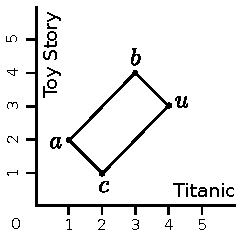
\includegraphics[width=2.5in]{figures/analogical_recommendation.pdf}
  \caption{Four users $a, b, c, u$ that are in proportion.}
\label{FIG:analogical_recommendation}
\end{figure}

\begin{table}[h!]
\centering
  \begin{tabular}{| c |  c  c  c  c  c | }
\toprule
 & $j_1$ & $j_2$ & $j_3$ & $\cdots$ & $i$\\
  \midrule
$a$ & 1 & 4  & 3 & $\cdots$ & 2 \\
$b$ & 5 & 2  & 3 & $\cdots$ & 4 \\
$c$ & 1 & 5  & 3 & $\cdots$ & 3 \\
$u$ & 5 & 3  & 3 & $\cdots$ & ? \\
\bottomrule
\end{tabular}
\caption{The four users $a, b, c, u$ are in proportion for every item $j$ that
  they have commonly rated. For an item $i$ that $u$ has not rated, the
  prediction $\predrui$ is set as the solution of the analogical equation
  $2:4::3:?$, i.e. $\predrui = 3 - 2 + b = 5$, using the arithmetic proportion.}
\label{TAB:analogical_recommendation}
\end{table}

Just like with the conservative classifier, we are facing the problem that in
practice, we may not find any $3$-tuple $a, b, c$ such that a perfect
proportion stands between $a, b, c$ and $u$. We will thus allow some distortin
of shape for the parallelogram $abcu$ by choosing another condition, for
example that $\norm{}{(a-b) - (c-u)} \leq \lambda$, where $\lambda$ is a
suitable threshold and $\norm{}{\cdot}$ is any $p$-norm. Note that this
relaxing of the definition of an analogical proportio exactly corresponds to
the usage of an analogical dissimilirity, so technically our algorithm is very
close to that of an extended classifier.

Our analogical proportion-based algorithm for recommendation is described by
Algorithm \ref{ALGO:analogical_recommendation}.
 \begin{algorithm}[!ht]
       \begin{algorithmic}

      \STATE {\bf Input}: A set of known ratings $R$, a user $u$, an item
      $i$ such that $r_{ui} \notin R$.
      \STATE {\bf Output}: $\hat{r}_{ui}$, an estimation of $r_{ui}$.

      \STATE {\bf Init}:
      \STATE $C = \varnothing$ \quad \quad // the set of candidate ratings
      \FORALL{
        users $a, b, c$ such that:\\
        \begin{itemize}
        \item $r_{ai} \in R, r_{bi} \in R, r_{ci} \in R$.
        \item $\norm{}{(a-b)-(c-d)}\leq \lambda$
        \item $r_{ai} : r_{bi} :: r_{ci} : y$ is solvable
        \end{itemize}
      }

      \STATE  $y \leftarrow r_{ci} - r_{ai} + r_{bi}$
      \STATE $C \gets C \cup \set{y}$ \quad // add $y$ as a candidate rating
	  \ENDFOR

    \STATE $\hat{r}_{ui} = \aggr{y \in C} y$

\end{algorithmic}
     \caption{Analogical proportion-based algorithm for recommendation.}
       \label{ALGO:analogical_reco}
\end{algorithm}

We will note here an important point: while an extended classifier would look
for the $k$ $3$-tuples with the least values of analogical dissimilarity, we
here look for all three tuples whose AD is below some given threshold. This is
a common variant of the $k$-NN algorithm: you can either look for the $k$
nearest neighbors, or look for all instances that are within a given distance.

We have considered a strict condition for the solvability of the equation
$r_{ai} - r_{bi} = r_{ci} - y$: as the exact arithmetic result $y=r_{ci} +
r_{bi} -r_{ai}$ does not necessarily belong to the rating scale used in our
experiments (which is $[1,5]$), we have
considered that the equation is solvable only when $r_{ai}=r_{bi}$ or
$r_{ai}=r_{ci}$. In both cases, we ensure the solution $x \in
[1,5]$.\todo{tester avec juste appartenance}

Another modification to the algorithm would be to only search for the users
$a, b,$ and $c$ in a subset of $U$. One may consider the set of the $k$-nearest
neighbours of $d$, using the assumption that neighbours are the most relevant
users to estimate a recommendation for $d$.

Just like for the neighborhood approach described earlier, it is perfectly
possible to apply this algorithm in an in an item-based way rather
than in a user-based way. I.e. instead of looking for $3$-tuples of users, we
may look for $3$-tuples of items, etc. Both views will be considered in our 
experimentations.


\subsection{Experiments and results}
\label{results}

Our algorithm \textit{Analogy} ($k=20$) is compared to the neighbourhood-based
algorithms model and \textit{Bsln-kNN} for the extended model using a baseline
predictor. For each of the algorithms, we have estimated the metrics described
in section \ref{TODO}.  The recommendation strategy $S$ that we have chosen is
to recommend $i$ to $u$ if $\hat{r}_{ui} \geq 4$.

We have tested and compared our algorithm on the Movielens-100K
dataset\footnote{http://grouplens.org/datasets/movielens/}, composed of 100,000
ratings from 1000 users on 1700 movies. Each rating belongs to the interval
$[1, 5]$.

In order to obtain meaningful measures, we have run a five-folds
cross-validation procedure: for each of the five steps, the set of ratings $R$
is split into two disjoint sets $R_{train}$ and $R_{test}$, $R_{train}$
containing four times more ratings than $R_{test}$. The reported measures are
averaged over the five steps. Naturally, the folds are the same for each of the
algorithms, to allow for meaningful comparisons.

Table \ref{table:res} shows the performances of the algorithms applied in a
user-based way. Similar experiments have been led in a movie-based setting,
exhibiting very similar results, slightly worse for RMSE (about 5\permil
higher).

\begin{table}[ht]
\begin{tabular}{| c || c | c | c | c | c | c | c | c |}
\hline
& RMSE & Prec & Rec & Cov & $Surp^{max}$ & $Surp^{avg}$ & Time \\
\hline
Analogy   & .898 & 89.1 & 43.3 & 31.2 & 0.433 & 0.199 & 2h \\
%Pattern & .927 & 84.9 & 50.0 & 47.7 & 0.433 & 0.198 & 5h \\
kNN     & .894 & 89.1 & 44.1 & 27.8 & 0.432 & 0.198 & 10s \\
Bsln-kNN & .865 & 88.4 & 44.0 & 44.7 & 0.431 & 0.199 & 10s \\
\hline
\end{tabular}

\caption{Performance of algorithms}
  \label{Zob}
\end{table}

As expected, the Bsln-kNN algorithm is more accurate than the basic
collaborative filtering method (KNN). The two classical collaborative
algorithms perform better than the new proposed analogy-based method in terms
of RMSE. Still, there seems to be some room for improvement for the analogical
approach, with the help of a careful analysis of the behaviour of the
algorithm.

As for performances other than RMSE, we see that the figures obtained by the
three algorithms are quite close. Regarding surprise, which is a delicate
notion to grasp, one may also wonder if the used measure is fully appropriate.

As usual, analogy-based algorithms suffer from their inherent cubic complexity.
In the case of recommender systems where millions of users/items are involved,
this is also a serious issue.

\section{Clones}

Considering analogy between four users has shown to be computationally
intensive, thus not really suitable for recommendation purposes, where time is
a highly critical dimension. Yet, other forms of analogy can be addressed in
the recommendation task, based on the observation that some users may be more
inclined to give good (or bad) ratings than others. Indeed, ratings are in no
way absolute and greatly depend on the subjective appreciation each user has
about the rating scale. In the $[1, 5]$ scale for example, two users $u$ and
$v$ might semantically agree on an item $i$ describing it as $bad$, but there
is a chance that this agreement is not perfectly reflected in the ratings: $u$
might have rated $i$ with $r_{ui} = 1$ and $v$ with $r_{vi} = 3$, simply
because from $v$' point of view $3$ is a \textit{bad} rating, while for $u$ a
rating of $3$ would simply mean \textit{decent} or \textit{good enough}.  In
the following, we refer such users that \textit{semantically} agree on their
common items (but not necessarily \textit{numerically}) as \textit{clones}, as
illustrated in Figure \ref{FIG_CLONES}. Please note that the word $clone$ is
not used here to mean \textit{strictly identical}, but more in the sense that
two clones are two users following parallel paths.

\todo{use nicer colors for plot?}
\begin{figure}[!h]
\centering
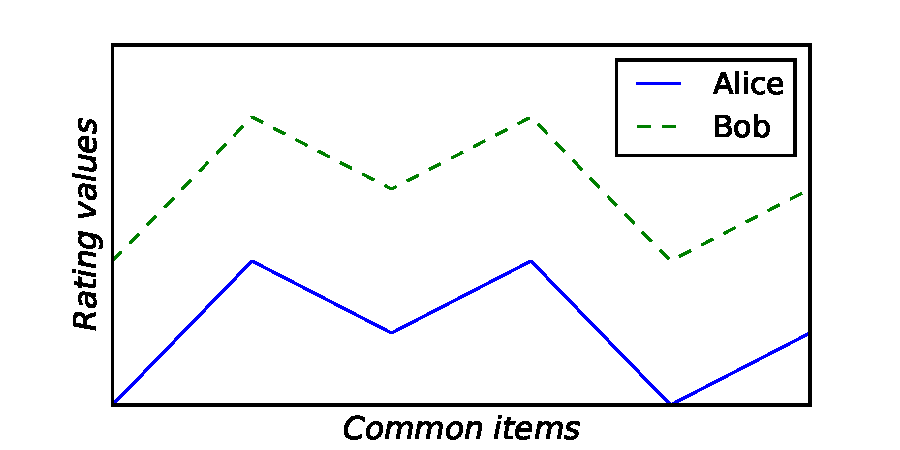
\includegraphics[width=4in]{figures/clones.pdf}
\caption{Bob is a perfect clone of Alice.}
\label{FIG_CLONES}
\end{figure}

It is obvious that in collaborative filtering, clones are of great interest when
it comes to predict a user's ratings, and yet the information they provide is
often discarded.  The principle underlying the analogical clone-based view is
the following: for predicting a missing rating for $u$ we not only look at its
nearest neighbors, but also to those $v$ whose rating are such that $r_{ui} =
r_{vi} + t_{vu}$ where $t_{vu}$ is a more or less constant \textit{correction
term} that can be either positive or negative.

In the next two sections, we investigate this idea of a clone-based prediction,
first when ratings are viewed as numerical quantities in section
\ref{NUMERICAL_POV}, and then when they have an ordinal meaning only in
section \ref{ORDINAL_POV}.

\subsection{Ratings as numerical quantities}
\label{NUMERICAL_POV}

In the following, we define $C_i(u)$ as the set of users that are clones of $u$
and that have rated item $i$.  From the previous definitions, one can easily
derive a very general collaborative filtering framework for predicting a user's
rating by taking into account its clones:
$$\predrui = \text{aggregation}(r_{vi} + t_{vu}), \quad \forall v \in
C_i(u),$$
where $t_{vu}$ is a \textit{correction term} that we need to add to $v$'s
ratings so that they correspond to those of $u$. We clearly have a
generalization of the $k$-NN approach, which we could write as:
$$\predrui = \text{aggregation}(r_{vi} + t_{vu}), \quad \forall v \in \{v \in C_i(u)
  | t_{vu} = 0\}.$$

Following this general framework, one can construct a great variety of
algorithms with various level of complexity. In the next subsections, we
propose a very straightforward algorithm, and a more efficient one.

\subsubsection{A straightforward prediction algorithm}
\label{STRAIGHTFORWARD}

In its most simple form, a user $v$ can be considered to be a $t$-clone of $u$ if
the ratings of $v$ differ from those of $u$ from a constant $t$:
\begin{equation}
v \in t\text{-}C(u) \iff \forall i \in I_{uv}, r_{ui} = r_{vi} + t.
\end{equation}
From then on, computing $\predrui$ amounts to finding all the users $v$ that
satisfy this criteria, and computing an aggregation of their rating for $i$,
which can simply be a mean. We implemented this basic algorithm described by
algorithm \ref{algo_straight}, and referred to as \textit{Bruteforce}.

 \begin{algorithm}[!ht]
   \caption{\textit{Bruteforce}}
       \label{algo_straight}
       \begin{algorithmic}

      \STATE {\bf Input}: A set of known ratings $R$, a user $u$, an item
      $i$ such that $r_{ui} \notin R$.
      \STATE {\bf Output}: $\hat{r}_{ui}$, an estimation of $r_{ui}$

      \STATE {\bf Init}:
      \STATE $C = \varnothing$ \quad \quad // list of candidate ratings
      \FORALL{ users $v \in U_i$}
        \FORALL{$t$}
          \IF{$v \in t\text{-Clones}(u)$}
          \STATE $C \gets C \cup \{r_{vi} + t\}$ \quad // add x as a candidate rating
          \ENDIF
        \ENDFOR
	    \ENDFOR
    \STATE $\hat{r}_{ui} = \aggr{x \in C} x$
\end{algorithmic}
\end{algorithm}

Of course, one may want to relax the definition of a $t$-clone, as the current
one is too strict and only very few users will satisfy this criteria. In our
implementation, we chose the following condition:
$$v \in t\text{-}C(u) \iff \sum_{i \in I_{uv}} |(r_{ui} - r_{vi}) - t| \leq |I_{uv}|.$$
This amounts to accept $v$ as a $t$-clone of $u$ if on average, $r_{ui} -
r_{vi}$ is equal to $t$ with a margin of $1$.

The values of $t$ clearly depend on the rating scale. The dataset on which we
tested our algorithms use the $[1, 5]$ interval, so possible values for $t$
that were considered are integer values between $[-4, 4]$.

This is obviously a very rough algorithm, to which one could point out numerous
flaws, but its purpose is to show that even such a basic clone-based approach
can lead to better results than a basic neighborhood method.

\subsubsection{Modeling clones with the similarity measure}
\label{MODELING_CLONES}
Another option to consider clones is to use the well known neighborhood-based
formula, and capture their effect inside an appropriate similarity measure. The
general neighborhood formula is as follows \cite{RecoSystemHandbook}:

$$\predrui = \frac{\sum_{v \in N_i^k(u)} r_{vi} \cdot sim(u, v)}{\sum_{v \in
  N_i^k(u)} sim(u, v)},$$
where $N_i^k(u)$ is the set of the $k$ nearest neighbors of $u$ that have rated
$i$. So, we move from a crisp view of the set of clones to a fuzzy one. In
fact, the above formula looks very similar to the interpolation principle
underlying Takagi-Sugeno fuzzy controller where similarity degree is viewed as
a fuzzy membership grade \cite{TakSug85}.

The above formula is commonly used with classical similarity metrics such as
Pearson or cosine similarity, or inverse of MSD (Mean Squared Difference, which is
a distance).
However, these similarities are not plainly satisfactory when it comes to
clones. Indeed with these metrics, two users are considered to be close if
their common ratings are often the same, but two perfect clones $u$ and $v$
with a significant correction term $t_{vu}$ would be considered as far from
each other, thus involving a loss of information.

A simple choice to measure how two users relate as clones can be the following:
$$Clone\_dist(u, v) =  \frac{1}{|I_{uv}|} \cdot \sum\limits_{i \in I_{uv}}
((r_{ui} - r_{vi}) - \mu_{uv})^2$$
where $\mu_{vu}$ is the mean difference between ratings of $u$ and $v$:
$$\mu_{uv}= \frac{1}{|I_{uv}|}\sum_{i \in I_{uv}} (r_{ui} - r_{vi}).$$

One can understand this distance in two ways:
\begin{itemize}
\item it can be regarded as the variance of the difference of ratings between
  $u$ and $v$,
\item or it can be regarded as a simple MSD measure ($\text{MSD}(u, v) =
  \frac{1}{|I_{uv}|} \cdot \sum\limits_{i \in I_{uv}}
  (r_{ui} - r_{vi})^2$)
 to which the mean difference of ratings between $u$ and $v$ has been
 subtracted.
  \end{itemize}

As our measure $Clone\_dist$ is a distance, it is necessary to transform it
into a similarity measure. Common choice is to take its inverse (while accounting for zero division): $Clone\_sim(u,
v) = \frac{1}{Clone\_dist(u, v) + 1}$.

Once we know how to find the clones of a user, it is a simple matter to output
a prediction using the classical neighborhood approach:
$$\predrui = \frac{\sum_{v \in N_i^k(u)} (r_{vi} + \mu_{uv}) \cdot sim\_clone(u,
v)}{\sum_{v \in N_i^k(u)} sim\_clone(u, v)}.$$

This algorithm will be referred to as $CloneA$. For the sake of completeness,
we also tried the same formula but with a more basic similarity metric that
does not care about clones: MSD. This algorithm is referred to as $CloneB$.

\subsubsection{ZOB}

A more sophisticated prediction, popularized by \cite{BelKorSIGKDD2007} is as
follows:
$$\predrui = b_{ui} + \aggr{v \in N_i^k(u)}(r_{vi} - b_{vi}),$$
where $b_{ui}$ is a baseline (or bias) related to user $u$ and item $i$. It
is supposed to model how $u$ tends to give higher (or lower) ratings than the
average of ratings $\mu$, as well as how $i$ tends to be rated higher or lower
than $\mu$. As it uses the neighbourhood of users to output a prediction, this
technique tends to model local relationships in the data.

Note that it is perfectly possible to proceed in an item-based way. Indeed,
rather than looking for users similar to $u$, one may look for items similar to
$i$, which leads to formulas dual of the above ones.


A simple and efficient formula using neighborhood technique, popularized by
\cite{KorACM2010} is the following:
$$\predrui = b_{ui} + \frac{\sum_{v \in N_i^k(u)} (r_{vi} - b_{vi}) \cdot
sim(u, v)} {\sum_{v \in N_i^k(u)}sim(u, v)}.$$
It is based on a simple $k$-NN approach, where are added the $b_{ui}$ terms,
called \textit{baselines}: $b_{ui} = \mu + b_u + b_i$. $\mu$ is the global mean
of all ratings in $R$. The $b_u$ term is intended to capture users propensity
to give ratings higher or lower than the global mean $\mu$, and the same goes
for items with $b_i$: some items tend to be rated higher than others. Baselines
are computed by solving a least squares problem:
$$ \min\limits_{b_u, b_i} \sum_{r_{ui} \in R} (r_{ui} - (\mu + b_u + b_i))^2,$$
which can be achieved efficiently by stochastic gradient descent, or
alternating least squares.

Among recommended similarity metrics, this one is of particular interest:
$$\text{sim}(u, v) = \frac
{ \sum\limits_{i \in I_{uv}} (r_{ui} -  b_{ui}) \cdot (r_{vi} - b_{vi})}
{\sqrt{\sum\limits_{i \in I_{uv}} (r_{ui} -  b_{ui})^2} \cdot
\sqrt{\sum\limits_{i \in I_{uv}} (r_{vi} -  b_{vi})^2}}.$$

It is simply a Pearson correlation coefficient, except that instead of
centering ratings by their means, they are centered with the baseline
predictors. An intuitive and illuminating way to look at this algorithm as a
whole is to see that it conceptually follows these steps:
\begin{enumerate}
  \item Compute $R'$, the set of all ratings normalized by the corresponding
    baseline: $r'_{ui} = r_{ui} - b_{ui}$.  $R'$ can be regarded as the set
    where all ratings are given from the same frame of reference, thus
    discarding any bias.  In $R'$, ratings can then be considered as absolute.
  \item Using $R'$, compute similarities between users using the cosine similarity (the
    cosine similarity is the same as the Pearson correlation coefficient,
    except that quantities are not centered).
  \item Output a prediction using the basic $k$-NN formula. As this prediction
    belongs to the same space of $R'$ where ratings have no bias, it needs to
    be transposed back to the space of $R$ (for performance evaluation
    purposes).
\end{enumerate}

In what follows, this algorithm is referred to as $k$-NNbsl.


It is very clear that the use of the baseline predictors is motivated by the
same reasons one would want to consider clones in a rating prediction
algorithms. This means that $k$-NNbsl implicitly takes the idea of clones into account, and thus a form of analogical reasoning.
Differences and resemblances of these two approaches are discussed
in the next section.

\subsubsection{Experiments and discussion}
\label{expeDiscuss}

We evaluated the performance of the aforementioned algorithms in terms of MAE
and RMSE on two datasets, the movielens-100K and movielens-1M
datasets\footnote{http://grouplens.org/datasets/movielens}, containing
$100,000$ and $1M$ ratings respectively. Results are shown in tables
\ref{table:res100k} and \ref{table:res1M} and where calculated using 5-folds
cross-validation. For each of these algorithms, the number of neighbors or
clones used to output a prediction is $k = 40$, except for the bruteforce
algorithm where the number of clones can not be controlled.
\begin{table}[!ht]
\centering
\caption{Performance of algorithms on the Movielens-100k dataset}
\label{table:res100k}
\begin{tabular}{| c || c | c | c | c | c | c |}
\toprule
     &  k-NN & Bruteforce & Clone A & Clone B & $k$-NNbsl\\
\midrule
RMSE & .9763 &   .9461    &   .9353 &  .9311  &  .9338   \\
MAE  & .7705 &   .8576    &   .7327 &  .7321  &  .7337   \\
\bottomrule
\end{tabular}
\end{table}

\begin{table}[!ht]
\centering
\caption{Performance of algorithms on the Movielens-1M dataset}
\label{table:res1M}
\begin{tabular}{| c || c | c | c | c | c | c |}
  \toprule
     &  k-NN & Bruteforce & Clone A & Clone B & $k$-NNbsl\\
  \midrule
RMSE & .9216 &           .&   .8996 &  .8969  &  .8879\\
MAE  & .7252 &           .&   .7057 &  .7050  &  .7005\\
\bottomrule
\end{tabular}
\end{table}

It is very clear that even a very straightforward approach of the clone-based
recommendation principle significantly outperforms the most basic $k$-NN
algorithm. It is however a lot heavier to compute, thus not very suitable for
real world recommendation purposes (its performances on the Movielens-1M
dataset simply could not be computed). The two other clone-based algorithms
however, have the exact same complexity of any $k$-NN-based algorithm which is
a significant improvement from the algorithm described in section
\ref{ANALOGY_USERS}.

Surprisingly enough, out of the two Clone algorithms, it is the one that does
not care about clones in its similarity measure that achieves the best results.
This might be due to the fact that in the neighborhood based on MSD, $\mu_{uv}$
is necessarily small and thus easier to estimate in a statistical significant
way.

Performances of the Clone algorithms are close to those of the state of the
art $k$-NNbsl algorithm. It is however important to understand that these
algorithms differ on the following points:
\begin{itemize}
\item The Clone algorithms do not address item bias, which is a significant
  drawback. It may not be unreasonable to believe that incorporating item bias
  in the prediction would lead to better results.
\item There is a subtle yet meaningful difference of interpretation between the
  biases induced by both algorithms. In the clone algorithm, biases are all
  pairwise, meaning that they involve two users, and they are computed on items
  that both users have rated. As for the $k$-NNbsl algorithm, there is no such
  thing as a pairwise bias. Bias for a given user is computed using only its
  own ratings, and is a result of a global optimization problem involving the
  global mean of all ratings, which means that every single rating in $R$ has
  an impact on the bias.
\item On the biggest dataset (Movielens-1M), the $k$-NNbsl algorithm appears to
  achieve better accuracy than the other algorithms, while this is not the case
  for the small dataset. A possible explanation is that as baselines are
  computed on the whole training set, they tend to capture most of the noise
  when the training set gets bigger, thus improving accuracy compared to more
  heuristic-based approach.
\end{itemize}

It should also be noted that in fact, it is recommended to perform a shrinkage
on the similarity measure of algorithm $k$-NNbsl, in order to take into account
the number of common items between two users: the more items they share, the
more confident we are when computing their similarity \cite{KorACM2010}. Such
an approach can improve significantly both RMSE and MAE of the algorithm.
Similarly, in the clone-based approach, it might be of interest to discount
clones that rely on a too small number of common items.

\subsection{Towards an ordinal view of ratings}
\label{ORDINAL_POV}

We may wonder if one can devise a counterpart of the numerical clone-based
approach, which would be compatible with an ordinal view of the ratings.
Indeed, an extreme way for unbiasing and comparing two sets of ratings is to
forget about their numerical values, and only consider their rankings.  The
idea of viewing ratings in a ordinal manner has been advocated in
\cite{KorSillRECSYS11}.
In this section, we discuss an ordinal counterpart of the analogical approach
previously presented.  Analogical reasoning with ordinal data has first been
proposed in \cite{MicBarCAP09}, yet with a different concern.

\subsubsection{An algorithm for rank prediction}
Indeed the idea that ``\textit{the rating of user $u$ for item $i$ is to the
rating of user $v$ for item $i$ as the rating of user $u$ for item $j$ is to
the rating of user $v$ for item $j$}’’ may be understood  as well in an ordinal
manner. This leads to state that ``\textit{the relative ranking of item $i$
  among the ratings given by user $u$  is to the relative ranking of item $i$
  among the ratings given by user $v$ as the relative ranking of item $j$ among
  the ratings given by user $u$  is to the relative ranking of item $j$ among
the ratings given by user $v$}.

This means that we need to compare the rankings given by two users $u$ and $v$
on their common items. In the following, $\rho_{ui}$ denotes the relative
ranking of item $i$ out of all the items rated by $u$. Our goal is to estimate
all values of $\rho_{ui}$, for any user and any item. The main steps of a
possible algorithm is as follows:
\begin{enumerate}
  \item Compute similarities between users, based on their rankings. A very
    popular similarity ranking measure is the Spearman's rank correlation
    coefficient, or Spearman's rho.
  \item Compute an estimated rank $\hat{\rho}_{ui}$ as an aggregation of all the
    rankings $\rho_{vi}$ extracted from the $k$ nearest neighbors (using
    Spearman's rho as similarity):
    $$\hat{\rho}_{ui} = \frac{\sum_{v \in N_i^k(u)} \rho_{vi} \cdot
    sim(u, v)}{\sum_{v \in N_i^k(u)} sim(u, v)}.$$
\end{enumerate}

This is obviously very similar to the neighborhood approach described in
section \ref{MODELING_CLONES}, but instead of predicting a rating, we output a
predicted rank. This approach is denoted as \textit{RankAnlg}.


\subsubsection{Experiments}

We evaluated the performance of our algorithm and compared it to other
previously described approaches, using the exact same evaluation protocol as in
section \ref{expeDiscuss}. The Movielens-1m dataset was not benchmarked, as our
algorithm is too computationally intensive.

RMSE and MAE are good measure for evaluation rating prediction accuracy, but
are not suitable when it comes to evaluate rankings. A better measure is the
Fraction of Concordant Pair, which evaluates the probability that given any two
items $i$ and $j$ rated by any user $u$, the system has correctly estimated
whether $u$ prefers $i$ over $j$ or the inverse. To compute the FCP, we need to
intermediate measures. $c_u$ defines the number of concordant pairs for user
$u$, and $d_u$ its number of discordant pairs. The FCP is then computed over all
users as the proportion of concordant pairs.

\begin{align*}
&c_u = \{(i, j) \in I^2 \quad s.t. \quad \predrui > \predruj \text{ and }
r_{ui} > r_{uj}\}\\
&d_u = \{(i, j) \in I^2 \quad s.t. \quad \predrui \geq \predruj \text{ and }
r_{ui} < r_{uj}\}\\
&FCP = \frac{\sum\limits_{u \in U} c_u}{\sum\limits_{u \in U} c_u + \sum\limits_{u \in U} d_u}
\end{align*}
Note that $\predrui$ here may represent either a rating prediction or a
ranking prediction $\hat{\rho_{ui}}$.

Results are reported in table \ref{table:res100kRank}.

\begin{table}[!ht]
\centering
\caption{Performance of algorithms on the Movielens-100k dataset (ranking
evaluation)}
\label{table:res100kRank}
\begin{tabular}{| c || c | c | c |}
\toprule
     & RankAnlg &  k-NN & $k$-NNbsl\\
\midrule
FCP  &  .7063   & .7096 &  .7163   \\
\bottomrule
\end{tabular}
\end{table}

Unfortunately, even a basic algorithm that was not designed for ranking
prediction performs better in terms of FCP. To explain this difference, one may
look at the distribution of average support over all the predictions, as shown
on figure \ref{FIG_SUPPORT}. Between
two users $u$ and $v$, the support is defined as the number of common items
($|I_{uv}|$), which was used to compute the similarity between $u$ and $v$. For
a given prediction $\predrui$, the average support is the average of all the
supports $|I_{uv}|$ over all users $v \in N_i^k(u)$.

\begin{figure}[!h]
\centering
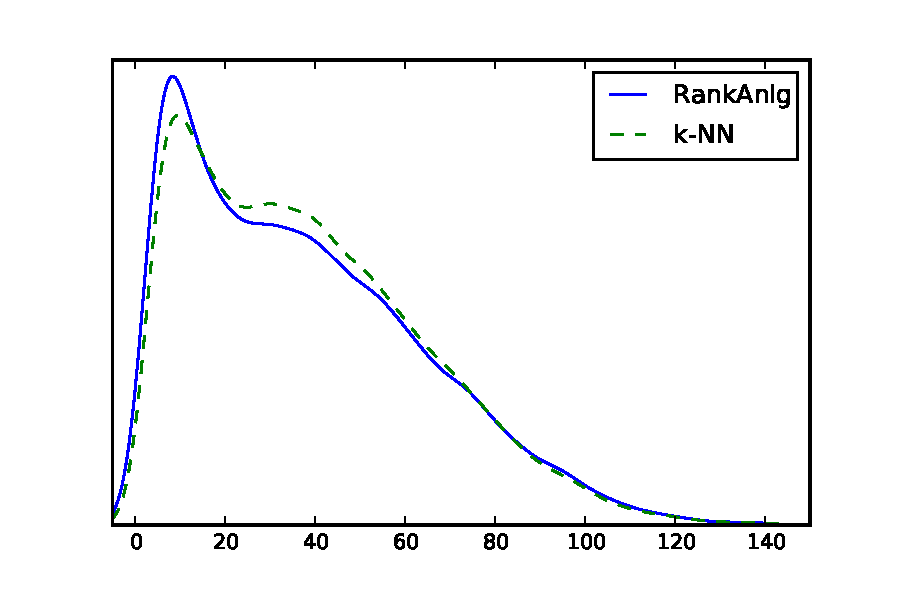
\includegraphics[width=2.5in]{figures/support.pdf}
\caption{Distribution of average support.}
\label{FIG_SUPPORT}
\end{figure}

The use Spearman's rho tends to provide with neighbors that have smaller
support, thus leading to a less significant and less accurate estimation of the
neighborhood, which may explain the differences in performance.

\section{Mining analogical proportions}

\subsection{Règles d'association}
Les règles d'association sont des informations extraites d'une base de
données qui révèlent des dépendances entre produits (aussi appelés
items).  Par exemple, partant
de la règle d'association $a \rightarrow b$  (si on achète $a$ alors il y a
de grandes chances que l'on achète $b$), un système de recommandation peut
suggérer $b$ dès lors qu'on a acheté $a$ mais pas encore $b$.  On définit
une règle d'association comme suit:

Soit $I= \{i_1,i_2,...,i_m \}$ un ensemble d'items. Soit $T= \{t_1, t_2,...,t_n
\}$ un (multi)-ensemble de transactions, i.e.,  $t_i \subseteq  I$. Une règle
d'association s'exprime sous la forme $X \rightarrow Y$ o\`u $X \subset I ,~ Y
\subset I, $ et $X \cap Y = \emptyset$.  $X$ et $Y$ sont des ensembles d'items
(appelés par la suite \textit{itemsets}), et le \emph{support} $supp(X)$ d'un
itemset $X$ est défini comme la proportion de
transactions qui le contiennent.  Un certain nombre de mesures permettent
d'\'evaluer la {\it qualité} d'une règle d'association, comme  la
\emph{confiance} qui s'exprime sous la forme $\frac{supp( X \cup Y)}{supp(X)}$.

Les méthodes d'extraction de telles règles ont fait l'objet de nombreuses
études. L'algorithme {\it Apriori}
\cite{AgrSriVLDB94} est probablement le plus connu mais il en existe d'autres.
L'idée   est de fixer un seuil minimum $\alpha$ pour le support et de chercher dans
$2^I$ les itemsets dont le support dépasse $\alpha$, pour obtenir un ensemble
$S$ d'itemsets fréquents. Cette recherche est facilitée par le fait que
tout sous-ensemble d'un itemset fréquent est aussi fréquent.

On se fixe alors un nouveau seuil $\beta$ pour la confiance.  Dès lors que
l'on dispose d'un itemset $IS$ de $S$, on peut chercher toutes les partitions
de $IS$ sous la forme $X \cup Y = IS$, calculer la confiance de la règle $X
\rightarrow Y$, ne garder cette règle que si sa confiance dépasse le seuil
$\beta$.

L'algorithme retourne finalement un ensemble de règles d'association
respectant les critères de qualité exigés, et fournissant donc un certain
nombre d'informations sur les liens entre les éléments de la base de
données.
%Sur le mode des proportions analogiques, on admettra que {\it le dentifrice
%est à la brosse à dent ce que le beurre est à la biscotte}.  Dans ce
%cas, on peut penser recommander à quelqu'un ayant acheté dentifrice,
%brosse à dent et beurre, d'acheter des biscottes. Sur quelle base?  Sur la
%base que la relation liant dentifrice et brosse à dent est la même que
%celle liant beurre et biscottes.
Au même titre que les règles d'association, la détection de proportions
analogiques dans une base de données est une information supplémentaire
fournie aux détenteurs de la base.  Dans la section suivante, nous
utilisons l'algorithme {\it Apriori} pour extraire d'une base des proportions
analogiques.

\subsection{Trouver des analogies}
Dans la suite, on recherche des analogies dans une base de données dédiée à la
recommandation.
L'objectif d'un système de recommandation est de fournir à un utilisateur une
liste personnalisée d'articles susceptibles de l'intéresser.  Soit $U$ un
ensemble d'utilisateurs et $I$ un ensemble d'items. Pour certaines paires $(u,
i) \in U \times I$, on connait la note $r_{ui}$, qui exprime l'intérêt que
l'utilisateur $u$ porte à l'item $i$ : on trouvera souvent $r_{ui} \in
[\text{aime, n'aime pas}]$ ou bien $r_{ui} \in [1, 2, 3, 4, 5]$. Nous dénotons l'ensemble des notes
connues du système par $R$.
% Pour recommander des articles aux utilisateurs, un
%système de recommandation procède ainsi: i) avec un algorithme $A$, on estime
%les notes $r_{ui}$ inconnues (c.à.d.  $r_{ui} \notin R$);
%Cette estimation  $A(u, i)$ est communément notée $\hat{r}_{ui}$.
%ii) Avec une stratégie de recommandation $S$ et au vu des notes précédemment
%estimées, recommander des items aux utilisateurs.
%Par exemple, une stratégie très basique mais assez courante est de suggérer à
%$u$ les articles $i$ pour lesquels $\hat{r}_{ui}$ est le plus grand.


Notre approche s'applique donc au cas o\`u peu de notes sont connues.  Considérons
4 items  $A, B, C$ et $D$ pour lesquels on cherche à savoir s'ils constituent
une analogie valide, sans avoir pour l'instant d'idée sur l'ordre dans lequel
on doit les considérer. Comme pour les règles d'association, la notion de
support demeure puisque ces 4 items constituent un 4-itemset.  Par
définition:

%\small
$Supp(\{A, B, C, D \})= \frac{|U_{ABCD}|}{|U|}$, où $U_{ABCD}$ est l'ensemble
des utilisateurs qui ont conjointement noté $A, B, C,$ et $D$.

%Dans le cas d'une base de données de films comme MovieLens, le support de 4
%films $\{a, b, c, d \}$ est simplement la proportion d'utilisateurs ayant vu
%ces 4 films.
Naturellement, comme pour les règles d'association, on peut ne
s'intéresser qu'aux analogies dont le support est supérieur à un certain
seuil $\alpha$.  Ensuite, pour un itemset $\{A, B, C, D \}$ de support
supérieur au seuil $\alpha$ que l'on s'est fixé, et ayant à notre
disposition une relation analogique permettant d'affirmer si, par exemple,
$A:B::C:D$ est valide ou non, on cherche quelles sont les analogies possibles.

On sait qu'il y a 4! = 24 permutations possibles de $\{A, B, C, D \}$,
correspondant à 24 analogies possibles. Cependant, compte tenu des
propriétés de l'analogie, un certain nombre d'entre elles sont
équivalentes et mènent à 3 classes de 8 analogies équivalentes
représentées par:
\begin{itemize}
\item $A:B::C:D$
\item $A:B::D:C$
\item $A:D::C:B$
\end{itemize}
Il convient donc de ne chercher que ces trois classes d'analogies.  Pour ce
faire, on pourra se donner une fonction $f$ évaluant la qualité d'une
analogie, un autre seuil de qualité $\beta$, et ne retenir, parmi les trois
options possibles que celles dont la qualité dépasse le seuil $\beta$. Ce que
nous appelons la qualité ici joue le rôle de la confiance pour les règles
d'association.  En clair $A:B::C:D$ est retenue comme analogie  valide si et
seulement si $f(A:B::C:D) \geq \beta$.  A la fin de cette procédure, on obtient
donc un ensemble d'analogies qui représentent des relations entre quatre items.

\subsubsection{Exemples de fonction de qualité}
Tous les 4-itemsets considérés $A, B, C, D$ sont représentés par
des vecteur de notes.  La dimension de ces vecteurs est égale au nombre
d'utilisateurs ayant noté les quatre items.  Cela nous donne plusieurs options
pour mesurer la qualité d'une proportion $A:B::C:D$, qui dépend de la nature
des analogies considérées et donc implicitement de l'échelle de notes.

Dans le cas d'une échelle binaire ($r_{ui} \in [\text{aime, n'aime pas}]$), on
pourra choisir pour $f$ la proportion de composantes pour lesquelles l'analogie
tient parfaitement.  Si l'échelle est numérique, on dispose de plusieurs
techniques pour évaluer l'exactitude d'une proportion entre quatre réels, qui
donneront des valeurs entre 0 et 1. Là aussi, on peut envisager une
aggrégation de ces valeurs de vérité.  Toujours si l'échelle est réelle et en
utilisant la proportion arithmétique, on sait que $A, B, C, D$ forment un
parallèlogramme ssi l'analogie est parfaite. La qualité d'une analogie
$A:B::C:D$ est donc inversement proportionnelle à la déformation du
parallélogramme dans $\mathbb{R}^n$, que l'on peut calculer en termes de
distance euclidienne.  Enfin, en adoptant un point de vue statistique on peut aussi
s'intéresser à la probabilité d'observer $A:B::C:D$, et considérer que la
proportion est crédible si elle a peu de chance d'être dûe au hasard (voir
Section \ref{expe}).

\subsubsection{Algorithme}
L'algorithme d'extraction de règles analogiques est alors calqué sur le modèle
d'extraction de règles d'association : on se donne une fonction de qualité $f$,
et deux seuils $\alpha$ et $\beta$.

D'abord, on calcule tous les 4-itemsets de support supérieur au seuil $\alpha$
à   l'aide de l'algorithme \textit{Apriori}.  Pour chaque itemset retenu,
on calcule la qualité des trois formes possibles non équivalentes d'analogie, et on garde celles dont
la qualité dépasse le seuil $\beta$.

\begin{enumerate}
\item Entrée: une relation d'analogie, une fonction de qualité $f$, deux seuils
  $\alpha$ et $\beta$.
\item Calculer tous les 4-itemsets de support supérieur au seuil $\alpha$ à
  l'aide l'algorithm \textit{Apriori}.
\item Pour chaque itemset retenu, calculer, parmi les 3 formes possibles non
  équivalentes d'analogie, celles dont la qualité dépasse le seuil $\beta$.
\item Sortie : la liste des règles analogiques retenues.
\end{enumerate}

\subsection{Premières expériences}

Nous avons expérimenté cet algorithme sur la base de données
Movielens\footnote{http://grouplens.org/datasets/movielens/},
constituée de $100~000$ notes de $1700$ films par $1000$ utilisateurs. Chaque
note appartient à l'échelle $[1, 2, 3, 4, 5]$, mais nous l'avons ramenée à une
échelle binaire de la façon suivante : un utilisateur $u$ aime un film s'il lui
a attribué une note supérieure à $\mu_u$, où $\mu_u$ est la note moyenne que
$u$ donne aux films qu'il a vus.

En plus de choisir un critère de support minimal, nous avons aussi imposé un
support maximal : les films très populaires vus par beaucoup de monde font
généralement consensus (les gens les apprécient), et ont peu de chance de
construire des analogies intéressantes. Cela a de plus l'avantage de réduire
l'espace de recherche, et donc accélerer significativement la recherche de
4-itemsets. De plus, toujours dans le but d'éviter de construire des analogies
trop triviales, on ne retient pas les proportions de la forme $x:x::x:x$.

En choisissant un support minimal de 40 et un support maximal de 150, nous
obtenons les mesures de qualités (calculées comme la proportion d'analogies
parfaites) illustrées par la figure \ref{qualite}. Comme on peut le voir, la
meilleure proportion a une qualité d'environ $40$\%, ce qui peut paraître peu
convainquant. Néanmoins, en remarquant que pour une composante il y a 4 chances
sur 16 d'obtenir une analogie significative (on ignore les $x:x::x:x$), et en supposant que les composantes sont
indépendantes les unes des autres, le nombre de composantes pour lesquelles
l'analogie est vraie suit une loi binomiale de paramètres $\mathcal{B}(40,
\frac{1}{4})$, où $40$ est la dimension des vecteurs. Sous ces hypothèses, la
probabilité d'obtenir $40$\% ou plus d'analogies parfaites est de $0.026$, ce qui
tend à montrer qu'un tel quadruplet d'items reste significatif, en cela que la
proportion analogique observée a peu de chance d'être due au hasard.

\begin{figure}[h]
  \vspace{-0.4cm}
\caption{Qualité des proportions trouvées}
\label{qualite}
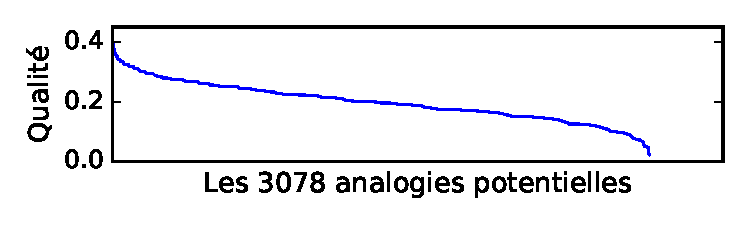
\includegraphics[scale=0.6]{figures/quality_of_proportions.pdf}
\vspace{-0.4cm}
\end{figure}
Les mêmes expériences ont été menées en gardant l'échelle de notes numérique
($[1, 2, 3, 4, 5]$) et en utilisant une expression multivaluée de l'analogie.
Les meilleures proportions obtenues s'avèrent être globalement les mêmes que
celles qui ressortent de l'échelle binaire, montrant ainsi la cohérence des
deux approches. La m\'ediocre qualit\'e des proportions analogiques trouv\'ees,
m\^eme si elles sont statistiquement significatives,
ne permet pas d'utiliser raisonnablement l'inf\'erence analogique dans cet exemple.
Ceci  tend \`a expliquer a posteriori pourquoi une approche pour la
pr\'ediction de notes manquantes, bas\'ee sur la recherche de triplets
analogiques, avait obtenu des r\'esultats modestes \cite{HugPraRicISMIS15}.


\chapter{Analogy-preserving functions}

\cite{HugPraRicSerECAI16} have proved that this kind of analogical
classification process can be formalized via two conceptual steps: first an
{\it analogical  extension} of the training set is performed (as detailed in
Section \ref{analogy}), and then a $k$-NN-like algorithm is applied to this
extended training set.  As expected, the accuracy of the analogical classifier
greatly depends on the quality of the extension. In this  paper, we introduce
the class of Analogy Preserving (AP) functions which ensure an error-free
extension.

Our paper is structured as follows. In Section \ref{extending} we overview
different methods currently used for extending a sample set.  In Section
\ref{analogy} we recall the basics of analogy and its counterpart in Boolean
logic (namely the analogical proportions), pointing out the existence of two
potential modelings. We also recall the process of
extending a sample set via analogy and introduce the notion of AP functions.
Section \ref{class_of_ap_functions} is devoted to a theoretical
characterization of AP functions. In section \ref{approximate_ap_functions} we
define and empirically investigate \textit{approximate} AP functions. We then
show their suitability for training set extension.

\section{Extending a training set}\label{extending}
Extension of a sample set (or training set) of a given universe $\mathcal{X}$
is a simple idea to improve generalization power. The more examples you have,
the better you learn! The point is then to add to the sample set $S$ some new
examples, but we have to do that in a way that preserves the \textit{quality}
of $S$.

Formally, we start with a set $S= \{x^{(i)} \in \mathcal{X}| i \in [1,n]\}$ of
examples ($n$ is supposed to be small), where $x^{(i)}$ is an
element of a Cartesian product $\mathcal{X} = X_1 \times \ldots \times X_m$.
For each element  $x^{(i)} \in S$, we associate a target  $f(x^{(i)})=y^{(i)}
\in Y$.  In the case of regression, $y^{(i)} \in \mathbb{R}$, and in the case
of classification $y^{(i)}$ belongs to a finite set and is called a class
or a \textbf{label}.

Several methods have been proposed for extending a sample set with new
examples. We may build a new example starting from
1, 2 or 3 known examples.
\begin{enumerate}
\item With one example, a natural way to proceed is to use the classical
  neighborhood approach: given one  example $(a,f(a))$, we can generate a new
    example $(b,f(b))$ where  $b$ is not too far from $a$ and $f(b)$ is not too
    far from $f(a)$. In the classification case, $f(b)$ may be chosen as
    $f(a)$.
\item With two examples, the previous option is still available and leads to
  interpolate the new example from the two given ones.  A somehow different
    option is the Feature Knockout procedure \cite{WolMar04}, which amounts
    to build a third example obtained by modifying a randomly chosen feature
    of the first example with that of the second one.  This way to
    proceed enjoys nice properties and appears to be equivalent to a popular
    regularization (Tikhonov) technique in the case of linear regression.  A
    related idea is used in a recent proposal \cite{BouPraRicECAI16} which
    introduces a measure of oddness w.r.t. a class that is computed on the
    basis of pairs made of two nearest neighbors in the same class; this is
    equivalent to replace the two neighbors by a fictitious representative of
    the class.

\item With three examples $(a,f(a)), (b,f(b)), (c,f(c))$, the previous options
  remain available and lead to build a fourth example which is somehow
    in-between the three other ones: we still have some kind of interpolation.
    A quite different idea is to extrapolate the fourth item on the basis of
    analogical proportion \cite{BayMouMicAnqECML07}.  In this perspective,
    this fourth element is not necessarily in the neighborhood of the three
    others.
\end{enumerate}
In this paper, we investigate this last option in depth.

\subsection{Analogy-preserving functions}\label{analogy-preserv}

\begin{definition}
  We say that $\mathbf{E}_S(f)$ is {\bf sound} if
  $\albl{\mathbf{x}}_f=f(\mathbf{x})$, for every $\mathbf{x} \in
  \mathbf{E}^*_S(f)$. Also, if $\mathbf{E}_S(f)$ is sound for all $S \subseteq
  \mathbb{B}^m$, we say that $f$ is {\bf Analogy Preserving} (AP).
\end{definition}

\noindent
Proposition \ref{equivalent_def} gives an equivalent definition of AP
functions.

\begin{proposition}\label{equivalent_def}
  A function $f \colon \mathbb{B}^m \to \mathbb{B}$ is AP iff for every
  $\mathbf{a}, \mathbf{b}, \mathbf{c}, \mathbf{d} \in \mathbb{B}^m$, $f$ suits
  the following requirement:
  $$
  \begin{cases}
    \mathbf{a} :  \mathbf{b} ::  \mathbf{c} :  \mathbf{d} \emph{ and }\\
  f(\mathbf{a}) :  f(\mathbf{b}) ::  f(\mathbf{c}) :  y \emph{ is solvable  }
  \end{cases}
  \implies y = f(\mathbf{d})
  $$
\end{proposition}
\begin{proof}
  If $f$ fulfills  this requirement, then it is clear from Section
  \ref{analogy-extension} that for any $S \subseteq
  \mathbb{B}^m$ and $\mathbf{x} \in \mathbf{E}^*_S(f)$, all the candidates $y$
  for $\albl{\mathbf{x}}_f$ are equal to $f(\mathbf{x})$, so
  $\albl{\mathbf{x}}_f$ will be invariably set to $f(\mathbf{x})$, which makes
  $f$ AP.

If $f$ does not suit this requirement, then there exist $\mathbf{a},
  \mathbf{b}, \mathbf{c}$, and $\mathbf{d} \in \mathbb{B}^m$ such that
  $\mathbf{a} : \mathbf{b} :: \mathbf{c} : \mathbf{d}$ but the solution $y$ to
  $f(\mathbf{a}) : f(\mathbf{b}) :: f(\mathbf{c}) : y$ is not equal to
  $f(\mathbf{d})$. Taking $S_0 = \{\mathbf{a}, \mathbf{b}, \mathbf{c}\}$ we
  obtain $\mathbf{E}^*_{S_0}(f) = \{\mathbf{d}\}$, and since $\albl{\mathbf{d}}_f = y
  \neq f(d)$, $\mathbf{E}_{S_0}(f)$ is not sound so $f$ is not AP.
\end{proof}

If $f$ is AP, then $\mathbf{E}_S(f)$ is sound for any $S$ so it is a relevant
extension of $S$ and can be used with full confidence for classification
purposes. In the rest of the paper, we will give a definite answer to the
following problem:

\begin{problem}\label{prob}
  Give a complete description of the functions $f\colon \mathbb{B}^m\to
  \mathbb{B}$ that ensure a sound extension $\mathbf{E}_S(f)$ for any sample
  set $S\subseteq \mathbb{B}^m$. In other words, identify all the AP
  functions.
\end{problem}

First note that many natural functions are not AP. Consider for example the
binary function $f(x_1,x_2)= x_1 \wedge x_2$, along with $\mathbf{a},
\mathbf{b}, \mathbf{c}, \mathbf{d} \in \mathbb{B}^2$ in Table
\ref{exampleNotAP}.  We have $\mathbf{a} : \mathbf{b} :: \mathbf{c} :
\mathbf{d}$ and $f(\mathbf{a}) : f(\mathbf{b}) :: f(\mathbf{c}) : y$ is
solvable, yet the solution is $y=0$, which  is different from $f(\mathbf{d})=1$
so $f$ is not AP. This actually comes from the fact that analogical proportions
are not stable by conjunction combination. It is also the case for the
disjunction \cite{PraRicLU13}.

\begin{table}[ht]
$\begin{array}{|c|cc|c|}
  \toprule
  ~ & x_1 & x_2 & f(\cdot) \\
  \midrule
  \mathbf{a} & 0 & 0 & 0\\
  \mathbf{b} & 0 & 1 & 0\\
  \mathbf{c} & 1 & 0 & 0\\
  \mathbf{d} & 1 & 1 & 1\\
  \bottomrule
\end{array}
$\bigskip
\caption{$f(x_1,x_2)= x_1 \wedge x_2$ is not AP.}
\label{exampleNotAP}
\end{table}

In the next section, we provide a complete description of AP functions and give
an answer to Problem \ref{prob}.

\section{The class of AP functions}
\label{class_of_ap_functions}

We first need to recall some basic notions in the theory of essential variables
of functions.

\subsection{Essential variables and sections of functions}

For $k\in [1,m]$, $\boldsymbol{\alpha}\in \mathbb{B}^m$, and $c \in
\mathbb{B}$, let ${\boldsymbol{\alpha}}_{k}^c$ be the tuple in $\mathbb{B}^{m}$
whose $i$-th component is set to $c$ if $i=k$, and to $\alpha_i$ otherwise.  A
variable $x_i$ is said to be \textbf{inessential} in $f\colon \mathbb{B}^m\to
\mathbb{B}$ if for all $\boldsymbol{\alpha} \in \mathbb{B}^m$ and $c \in
\mathbb{B}$, $f(\boldsymbol{\alpha}^c_i) = f(\boldsymbol{\alpha}^{\neg c}_i)$.
Otherwise, $x_i$ is said to be \textbf{essential} in $f$, or that $f$ depends
on $x_i$. In simple terms, an
essential variable is a variable that has the \textit{ability} to change the
value of $f$. For example in $f(x_1, x_2, x_3) = x_1 \wedge x_3$, $x_1$ and
$x_3$ are essential variables while $x_2$ is inessential.  We denote by
$\ess(f)$ the number of essential variables of $f$ (or \textbf{essential
arity}).

Two functions $f\colon \mathbb{B}^m\to \mathbb{B}$ and $g\colon \mathbb{B}^n\to
\mathbb{B}$ are said to be {\bf equivalent} if there exist two mappings
$\sigma\colon
[1,n]\to [1,m]$ and $\sigma'\colon [1,m]\to [1,n]$ such that
\begin{align*}
  f(x_1,\ldots , x_m)&=g(x_{\sigma(1)},\ldots,x_{\sigma(n)}) \text{ and} \\
   g(x_1,\ldots , x_n)&=f(x_{\sigma'(1)},\ldots,x_{\sigma'(m)}).
\end{align*}
In other words, $f$ and $g$ are equivalent if one can be obtained from the
other by permutation of variables, addition of inessential variables, or
identification of inessential variables. For example, $f(x_1, x_2, x_3) = x_1
\wedge x_3$ and $g(x_1, x_2)  = x_1 \wedge x_2$ are equivalent functions. Note
that two equivalent functions necessarily have the same number of essential
variables. For further background in the theory of essential variables of
functions, see \cite{CouceiroTCS08, CouceiroDM09, SalomaaAASF63, WillardDM96}.

In our demonstrations, we will use the following property:

\begin{property}\label{equivalent_functions}
Let $f\colon \mathbb{B}^m\to \mathbb{B}$ and $g\colon \mathbb{B}^n\to
  \mathbb{B}$ be equivalent functions. Then $f$ is AP if and only if $g$ is AP.
\end{property}

This can be verified by noting that as the analogy in $\mathbb{B}^m$ is defined
component-wise, the permutation of variables has no effect on the equation and
its solution. Also, manipulation of inessential variables do not change the
value of the function $f$, and thus the AP property still holds.

We now define the concept of \textbf{section} of a function, also known as a
\textit{restriction}, or equivalently as the result of \textit{partial
application} in computer science. Let $f$ be a function $\mathbb{B}^m\to \mathbb{B}$, and $(I,
J)$ be a partition of $[1, m]$. With $\mathbf{x}
\in \mathbb{B}^m$ and $\boldsymbol{\alpha} \in \mathbb{B}^{|I|}$, the $I$-section (or simply
section) $f^{\boldsymbol{\alpha}}_I \colon \mathbb{B}^{|J|} \to \mathbb{B}$ is the function that
is obtained after setting all variables in $I$ to the components of
$\boldsymbol{\alpha}$. Note that the arity of $f^{\boldsymbol{\alpha}}_I$ is
$|J|$, and that $\ess(f^{\boldsymbol{\alpha}}_I) \leq \ess(f)$.
For example, consider a function $f$ of three variables: $f(x_1,x_2, x_3) = (x_1
\wedge x_2) \lor x_3$. The section $f^{(1, 0)}_{\{1, 3\}}$ is defined as $f^{(1,
0)}_{\{1, 3\}}(x_2) = (1 \wedge x_2) \lor 0$.

A main result about sections that will be used in other proofs is stated in
Property \ref{section_preserve_wap}, which can be verified by noting that
$x:x::x:x$ for any $x \in \mathbb{B}$:

\begin{property}\label{section_preserve_wap}
If $f\colon \mathbb{B}^m\to \mathbb{B}$ is AP, then every section of $f$ is
also AP.  \end{property}

In the following, the AND operator `$\wedge$' will be denoted `$\cdot$' to fit
with an algebraic notation. Also, `$+$' will now denote the modulo-2 addition,
equivalent to the XOR operator. Note that $x + 1 = \neg x$.

\subsection{The affine functions}

We are now in a position to see some examples of AP functions. We will show that
any affine function is AP.

\begin{proposition}\label{affine_functions_are_wap}
Let $L$ be the class of all affine functions, i.e. functions of the form:
  $$f(x_1,\ldots , x_m)=\alpha_1\cdot x_1+\ldots +\alpha_m\cdot  x_m+\alpha,$$
  with $\alpha_1,\ldots, \alpha_m,\alpha\in \mathbb{B}$. Every affine function
  (also called linear when $\alpha = 0$) is AP.
\end{proposition}

\begin{proof}
Let $f \colon \mathbb{B}^m \to \mathbb{B} \in L$. Using the obvious fact that
  $f$ is AP  iff $f + 1 = \neg f$ is AP, we may assume without loss of generality that
  $\alpha = 0$. Also, considering that $f$ essentially depends on $n \leq m$
  variables ($n$ is then the number of $\alpha_i$ equal to $1$), $f$ is
  equivalent to the function $g \colon \mathbb{B}^n \to \mathbb{B}$ defined by
  $g(x_1, \cdots, x_n) = x_1 +  \cdots + x_n$. Using Property
  \ref{equivalent_functions}, we just need to prove that $g$ is AP to show that
  $f$ is also AP.

  This function $g$ has the remarkable property\footnote{This is the reason why affine
  functions lead to classification problems that are, in fact, highly
  \textbf{non} linearly separable.} that changing the value of any
  $x_i$ changes the value of $g$: $\forall _i, \quad g(x_1, \cdots, x_i, \cdots, x_n) =
  \neg g(x_1, \cdots, \neg x_i, \cdots, x_n)$. From this property, it is easy to
  see that:
  $$\forall \mathbf{x}, \mathbf{x}' \in \mathbb{B}^m, g(\mathbf{x}) =
  g(\mathbf{x}') \iff h(\mathbf{x}, \mathbf{x}') \text{ is even }$$
  where $h$ is still the Hamming distance function.

  Let $\mathbf{a}, \mathbf{b}, \mathbf{c}, \mathbf{d} \in \mathbb{B}^m$  such
  that the two hypothesis in the definition of AP are satisfied, i.e.
  $$
  \mathbf{a} : \mathbf{b} :: \mathbf{c} : \mathbf{d}\quad \text{and}\quad
  g(\mathbf{a}) : g(\mathbf{b}) :: g(\mathbf{c}) : y\quad  \text{is  solvable}.
  $$

  As the equation is solvable, Table \ref{truthTableAnalogy} tells us that
  there are three possibles cases (we will use Property
  \ref{hamming_analogy}):
  \begin{enumerate}
    \item $g(\mathbf{a}) = g(\mathbf{b})$, and in this case the solution is
      $y = g(\mathbf{c})$. As $g(\mathbf{a}) = g(\mathbf{b})$, then
      $h(\mathbf{a}, \mathbf{b})$ is even, and so is $h(\mathbf{c},
      \mathbf{d})$. Then, $g(\mathbf{c}) = g(\mathbf{d})$ so $y = g(\mathbf{d})$.
    \item $g(\mathbf{a}) = g(\mathbf{c})$, and in this case the solution is $y =
      g(\mathbf{b})$. As $g(\mathbf{a}) = g(\mathbf{c})$, then
      $h(\mathbf{a}, \mathbf{c})$ is even, and so is $h(\mathbf{b},
      \mathbf{d})$. Then $g(\mathbf{b}) = g(\mathbf{d})$ so $y =
      g(\mathbf{d})$.
    \item $\neg g(\mathbf{a}) = g(\mathbf{b}) = g(\mathbf{c})$, and in this
      case the solution is $y = g(\mathbf{a})$. As $g(\mathbf{b}) =
      g(\mathbf{c})$, then $h(\mathbf{b}, \mathbf{c})$ is even, and so is
      $h(\mathbf{a}, \mathbf{d})$. Then $g(\mathbf{a}) = g(\mathbf{d})$ so $y =
      g(\mathbf{d})$.
  \end{enumerate}

  The third case is only relevant for the Klein modeling. In all cases we have
  $y = g(\mathbf{d})$, thus showing that $g$ is AP, and so is any $f \in L$.
\end{proof}


\subsection{A complete description of AP functions}

We have seen that every affine function is AP. We will here give a stronger
result: the affine functions are the \textbf{only} AP functions.

For that we shall make use of the  polynomial representation of Boolean functions.
A \textbf{ monomial} is a term of the form:
$$
\mathbf{x}_I=\underset{i\in I}{\prod}x_i, $$ for some possibly empty finite set of
positive integers $I$, where $|I|$ is called the \textbf{degree} of
$\mathbf{x}_I$.   We take the convention that $1$ is the empty monomial
$\mathbf{x}_\emptyset $. A \textbf{ polynomial} is a sum of monomials and its
degree is the largest degree of its monomials.  It is well-known
\cite{StoneAlgebra36,ZhegalkinAlgebra27} that any function
$f:\mathbb{B}^m\rightarrow \mathbb{B}$ is uniquely represented by a polynomial,
also called the Algebraic Normal Form: $$f(x_1,\ldots,x_m)=\sum_{I\subseteq
\{1,\ldots,m\}}a_I\cdot \mathbf{x}_I$$ where each $a_I$ belongs to
$\mathbb{B}$. Note that the constant function $0$ is represented by
$a_\emptyset\cdot \mathbf{x}_\emptyset$ with $a_\emptyset =0$. The degree of a
function $f:\mathbb{B}^m\rightarrow \mathbb{B}$, denoted $d(f)$, is defined as
the degree of the unique polynomial representing $f$.

Note that the class of functions with degree at most $1$ is exactly the class
$L$ of affine functions, which are AP. We will show that the class of AP
functions is the class of affine functions by proving that if a function $f$ is
AP, then $d(f)\leq 1$. We first consider the case where $d(f) = 2$.

\begin{property} \label{degree_2_not_AP}
 Let $f\colon \mathbb{B}^m\to \mathbb{B}$ with $d(f)=2$. $f$ is not AP.
\end{property}
\begin{proof}
  Let's consider $f$ with $d(f) = 2$ and $\ess(f) >= 2$. We denote $\mathbf{x}_I$ one of the
  monomial of $f$ of degree $2$. We consider the section $f^{\mathbf{0}}_J$,
  where $J = [1, m] \setminus I$,  and $\mathbf{0}$ denotes the constant 0
  vector in $B^{|J|}$. All variables that are not part of the monomial
  $\mathbf{x}_I$ have been set to $0$. This section $f^{\mathbf{0}}_J$ has a
  unique monomial of degree $2$ (namely $\mathbf{x}_I$) and $\ess(f) = 2$.
  $f^{\mathbf{0}}_J$ is necessarily equivalent to one of the following
  functions:
  $$
  \begin{cases}
    f_1(x_1, x_2) = x_1 \cdot x_2 + \alpha \\
    f_2(x_1, x_2) = x_1 \cdot x_2 + x_1 + \alpha\\
    f_3(x_1, x_2) = x_1 \cdot x_2 + x_1 + x_2 + \alpha
  \end{cases}$$
  It is pretty straightforward to find examples of $\mathbf{a}, \mathbf{b},
  \mathbf{c}, \mathbf{d} \in \mathbb{B}^2$
  that show that none of these functions are AP, so $f^{\mathbf{0}}_J$ can't
  be AP either. As $f^{\mathbf{0}}_J$ is a section of $f$, $f$ cannot be AP.
\end{proof}

All we need now is a property that could allow us to decrease the degree of a
function without changing its AP property. This is the purpose of
Property \ref{section_degree_k_minus_1}.

\begin{property}\label{section_degree_k_minus_1}
Let $f:\mathbb{B}^m\rightarrow \mathbb{B}$ be a function with
  $d(f)=k\geq 2$. Then there is a section $g$ of $f$ with $d(g)=k-1$.
\end{property}
\begin{proof}
Suppose that  $d(f)=k\geq 2$, and let $\mathbf{x}_I$ be a monomial of $f$ of
  maximum degree, i.e. $|I|=k$.  Here again, consider the section $g =
  f^{\mathbf{0}}_J$ where $J = [1, m] \setminus I$ and $\mathbf{0}$ denotes the
  constant $0$ vector in $\mathbb{B}^{|J|}$. It is clear that $g$ is
  represented by a  polynomial that has a unique monomial of maximal degree
  $k$, namely $\mathbf{x}_I$, and maybe some other monomials of degree strictly
  less than $k$.  Let us choose any $i \in I$: then $g' = g^1_{\{i\}}$ is a
  section of $g$ of degree (and arity) $k-1$. As $g'$ is a section of $g$, it
  is also a section of $f$ which completes the proof.
\end{proof}

We are now in position to prove our main result.

\begin{proposition}\label{AP_is_L}
The class of AP functions is the class $L$ of affine functions.
\end{proposition}
\begin{proof}
We have seen that every affine function is AP, i.e. if $d(f)\leq 1$, then $f\in
  AP$. On the other hand, Property \ref{degree_2_not_AP} tells us that if
  $d(f)=2$, then $f \notin AP$. So suppose that  $d(f)\geq 3$. By successive
  applications of Property \ref{section_degree_k_minus_1}, it follows that
  there is a section $g$ of $f$ with $d(g)=2$.

  As $g$ is not AP, then $f$ is not AP either. All in all, if $d(f) \geq 2$
  then $f$ is not AP, so the class of AP functions is $L$.
\end{proof}

We can finally give a definite answer to our initial problem: {\bf the class of
functions that ensure a sound extension of any sample set $S \subseteq
\mathbb{B}^m$ is the class of affine functions $L$}. If the function is not
affine, then there exist a sample set $S \subseteq \mathbb{B}^m$ for which
$\mathbf{E}_S(f)$ is unsound.

Now, while this theoretical result is interesting on its own, it is obvious
that purely affine functions are not representative of what would be
encountered in a real-world environment.  This leads to {\bf Problem 2}: What
remains of the quality of the analogical extension $\mathbf{E}_S(f)$ when $f$
deviates from being AP in different ways?  The aim of the next section is to
empirically investigate this question.

\section{Approximately AP functions and experiments}
\label{approximate_ap_functions}

Given two Boolean functions $f$ and $g$, we define their distance
$\text{dist}(f, g) = P_\mathbf{x}\left[f(\mathbf{x}) \neq
g(\mathbf{x})\right]$, where $P_\mathbf{x}$ is the uniform distribution over
$\mathbb{B}^m$. Here, $\mathbf{x} \in \mathbb{B}^m$ is also considered as a
random variable. We say that $f$ is $\epsilon$-close to $g$ if $\text{dist}(f,
g) \leq \epsilon$, and that $f$ is $\epsilon$-close to $L$ if $\exists g \in L$
such that $f$ is $\epsilon$-close to $g$. Given a sample $S$, we define
$\omega$ as the quality of the extension $\mathbf{E}_S(f)$ with $\omega =
P_{\mathbf{x}\in \mathbf{E}^*_S(f)}\left[\albl{\mathbf{x}}_f =
f(\mathbf{x})\right]$. By definition, $\omega=1$ for all $S$ iff $f$ is AP.
Note that there exist statistical tests allowing the practitioner to query a
partially-known function to find out if it is $\epsilon$-close to L (see for
instance \cite{BluLubRub93}).\todo{BLR marche que pour fonctions lineaires
mais OSEF car omega de f = omega f + 1 et si f lineaire alors f + 1 est affine
donc on peut se contenter de BLR}. Therefore, studying $\omega$ w.r.t. $\epsilon$
is clearly of interest.

Starting from an affine function $g \colon \mathbb{B}^8 \to \mathbb{B}$ defined
as  $g(\mathbf{x}) = x_1 + \cdots + x_8$, we introduce some noise by negating
its output $g(\mathbf{x})$ with probability $\epsilon$. We thus obtain
functions $f_{\epsilon}$ that are $\epsilon$-close to $L$, and report the value
of $\omega$ averaged over $50$ experiments (using the Standard modeling).
Figure \ref{omega_vs_eps} gives an illustration of the variation of $\omega$
w.r.t.  $\epsilon$ for different sizes of $S$ (as a percentage of
$|\mathbb{B}^m|$).  Other experiments have been carried out with other affine
functions (i.e.  with less essential variables or different arity), leading to
very similar results.  Note that $\epsilon$ only needs to be taken in $[0,
\frac{1}{2}]$, because being $\epsilon$-close to $g$ is equivalent to be $1 -
\epsilon$-close to $g + 1 = \neg g$ which is still affine, so the curves are
symmetrical with respect to the axis $\epsilon = \frac{1}{2}$.

\begin{figure}
\begin{center}
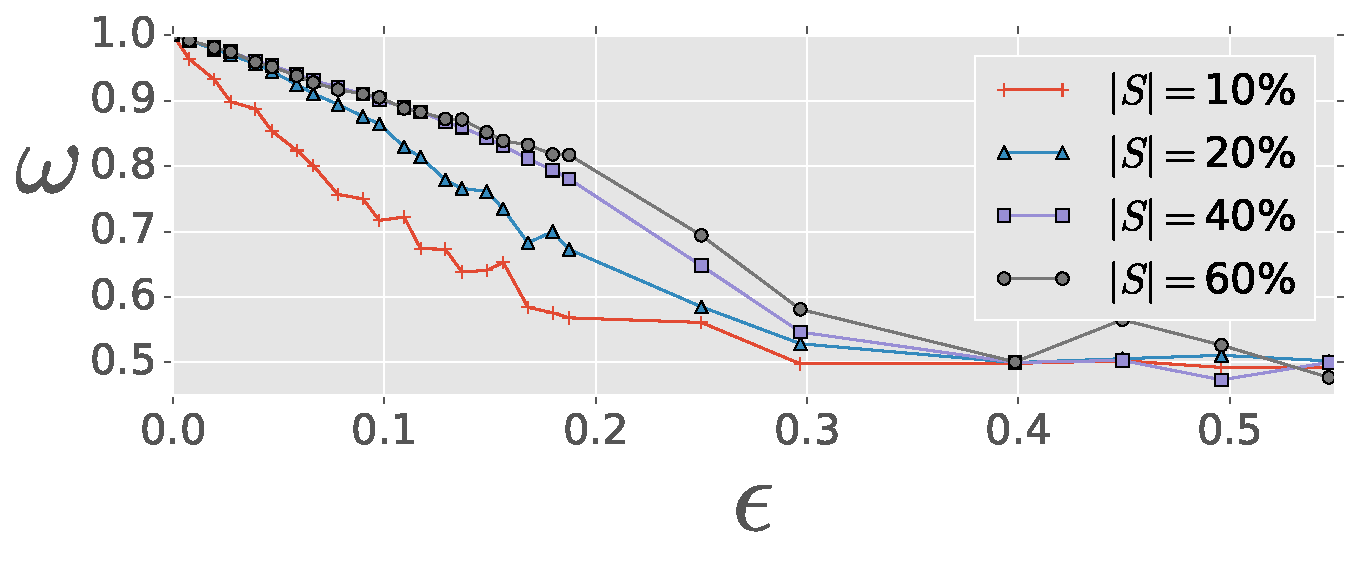
\includegraphics[scale=0.6]{figures/omega_vs_eps_dim8_nexp50_std_nEss8.pdf}
  \caption{$\omega$ for $\epsilon$-close functions to $L$.}
\label{omega_vs_eps}
\end{center}
\end{figure}

When $\epsilon = 0$ we get $\omega = 1$, as expected from
Proposition \ref{AP_is_L}. We observe an almost linear decrease in $\omega$ as
$\epsilon$ grows to $0.3$ then leading to a plateau where $\omega =
\frac{1}{2}$, indicating that the analogical labels $\albl{\mathbf{x}}_f$ are
more or less random. Moreover, $\omega$ appears to decrease faster for small
samples $S$. This is due to the fact that the analogical labels
$\albl{\mathbf{x}}_f$ are the result of a majority-vote procedure among the
candidate solutions that one can build from $S$, and the number of candidates
becomes smaller as $|S|$ decreases, thus altering the quality of the
prediction. The determination of a functional dependence between $\omega$,
$\epsilon$ and $|S|$ is currently being investigated.

Now, let us note the following point: even if a function $f$ is far from being
AP, the quality $\omega$ of the extension $\mathbf{E}_S(f)$ may still be very
high. To illustrate this, let us define the value $\beta$ which is an indicator
of how far is $f$ from being completely AP.  For each $\mathbf{x} \in
\mathbf{E}^*_S(f)$, we define $\beta_\mathbf{x}$ as the proportion of
candidates $y$ that led to the the correct label, i.e. the proportion of $y$
such that $y = f(\mathbf{x})$. $\beta$ is defined as the average of all the
$\beta_\mathbf{x}$.  Obviously, a function $f$ is AP iff $\beta = 1$ for all
$S$, i.e. if $\beta_\mathbf{x} = 1$ for all $\mathbf{x} \in \mathbf{E}^*_S(f)$
and for all $S$.

Table \ref{table_monks} reports the values of $\omega$ and $\beta$ for the
Standard and the Klein modelings of analogy (respectively $\omega_S$,
$\omega_K$, $\beta_S$ and $\beta_K$) over three datasets from the UCI
repository, namely the three Monk's problems\footnote{As these datasets are
nominally-valued, they are binarized.} \cite{UCIrepo}. Results are averaged
over 100 experiments, where the sample set $S$ is each time randomly sampled
with a size of $30$\% of the universe of possible instances.

\begin{table}
\centering
\begin{tabular}{| c | c | c | c | c |}
\toprule
  & $\omega_S$  & $\omega_K$ & $\beta_S$  &  $\beta_K$ \\
\midrule
Monk 1 & .96 & .96 & .73 & .62 \\
Monk 2 & .96 & .84 & .69 & .60 \\
Monk 3 & .98 & .95 & .87 & .77 \\
\bottomrule
\end{tabular}
\caption{$\omega$ and $\beta$ for the Standard and Klein modelings over the
  Monk's problems.}
\label{table_monks}
\end{table}

We observe that for each dataset, $\beta_S$ is significantly lower than $1$.
This suggests that the Boolean functions underlying these
datasets are highly not AP, because on average, there is a high proportion
(around $20$\%) of candidates $y$ that predicted the wrong label. However,
$\omega_S$ is no lower than $96$\%, implying extensions of very high quality.
This is where the majority-vote comes into play: in some cases, it may be able
to compensate for the predictors $y$ that were wrong.  This is what happens
here in $96$\%, $96$\% and $98$\% of the cases respectively. Here again,
obtaining theoretical guarantees about the majority vote procedure is currently
investigated.

We note also that the Klein modeling achieves equal or lower quality than the
standard one, which suggests that the Standard modeling, which has the same
class of AP functions, is more useful in practice. Note that such a difference
between $\omega_S$ and $\omega_K$ has been consistently observed over many
other experiments, which we do not mention here for lack of space. This may be
explained by the fact that, as mentioned earlier, the Klein modeling obeys
the following property, unnatural  for an analogy: $A_K(a, b, c, d)
\iff A_K(b, a, c, d)$.


\backmatter
\bibliographystyle{alpha} % or named ?
\refstepcounter{chapter}
\bibliography{biblio}

\end{document}
